%!TEX TS-program = xelatex
%!TEX encoding = UTF-8 Unicode
\documentclass[a4paper, 12pt, oneside]{book}

\usepackage{type1cm}
\usepackage{subfigure}
\usepackage{array}
\usepackage{tabu}
\usepackage{mathtools}
\usepackage{dcolumn}

\usepackage{cite}
%\usepackage{chapterbib}
%The chapterbib package facilitates multiple bibliographies in a LATEX document
\usepackage[hyphens]{url}
%Verbatim with URL-sensitive line breaks.
\usepackage[colorlinks=true,linkcolor=black,citecolor=black,filecolor=blue,urlcolor=blue,unicode]{hyperref}
%The hyperref package is used to handle cross-referencing commands in LaTeX to produce hypertext links in the document. The package provides backends for the \special set defined for HyperTeX DVI processors; for embedded pdfmark commands for processing by Acrobat Distiller (dvips and Y&Y’s dvipsone); for Y&Y’s dviwindo; for PDF control within pdfTeX and dvipdfm; for TeX4ht; and for VTeX’s pdf and HTML backends.
\usepackage{verbatim}
%The verbatim environment  simply reproduces every character you input, including all  s p a c e s!
\usepackage{color}
%you can set the color of the font of the text, and set the background color of the page.
\usepackage[dvipsnames]{xcolor}
%xecolor package is a simple package which defines about 140 different colors by XeTeX's font
\usepackage{graphicx}
%Standard LaTeX graphics.
\usepackage{array}
%The array environment is used to make a table of information, with column alignment (left, center, or right) and optional vertical lines separating the columns.
\usepackage{gensymb}
%Provides generic commands \degree, \celsius, \perthousand, \micro and \ohm which work both in text and maths mode.
\usepackage{indentfirst}
%Make the first line of all sections etc., be indented by the usual paragraph indentation. This should work with all the standard document classes. This minimalist package is part of the "tools" bundle in the LaTeX required distribution.
\usepackage{algorithm}
\usepackage{algpseudocode}
%A suite of tools for typesetting algorithms in pseudo-code. The algorithmicx package provides many possibilities to customize the layout of algorithms. You can use one of the predefined layouts (pseudocode, pascal and c and others), with or without modifications, or you can define a completely new layout for your specific needs.
\usepackage{enumitem}
%Control layout of itemize, enumerate, description.  It supersedes both enumerate and mdwlist (providing well- structured replacements for all their funtionality), and in addition provides functions to compute the layout of labels, and to 'clone' the standard environments, to create new environments with counters of their own.
\usepackage{mfirstuc}
%\makefirstuc{〈stuff 〉} This makes the first object of 〈stuff 〉 uppercase unless 〈stuff 〉 starts with a con- trol sequence followed by a non-empty group, in which case the first object in the group is converted to uppercase.
\usepackage{fancyvrb}
%This package provides very sophisticated facilities for reading and writing ver- batim TEX code.
\usepackage{amsfonts}
%TeX fonts from the American Mathematical Society.
\usepackage{ifmtarg}
%If-then-else command for processing potentially empty arguments.
\usepackage{amsmath}
%The amsmath package is a LATEX package that provides miscellaneous enhance- ments for improving the information structure and printed output of documents that contain mathematical formulas.
\usepackage{amssymb}
% Math symbols
\usepackage[mathcal]{euscript}
%This file sets up some font shape definitions to use the Euler script symbols in math mode.
\usepackage[notbib]{tocbibind}
%Add (or disable) bibliography/index/contents to Table of Contents.
\usepackage{rotating}
%Rotation tools, including rotated full-page floats.
\usepackage{hhline}
%The command \hhline produces a line like \hline, or a double line like \hline\hline, except for its interaction with vertical lines. The command takes a preamble (rather like the preamble of a tabular environment), and this specifies whether there are to be one or two horizontal lines, and what happens when the horizontal line meets a vertical one. The package is part of the tools bundle in the LaTeX required distribution.
\usepackage{wallpaper}
%Easy addition of wallpapers (background images) to LaTeX documents, including tiling.
\usepackage{pdfpages}
%Include PDF documents in LaTeX.
\usepackage{pst-fractal,pst-exa}
% The package will draw the Julia and Mandelbrot sets, the Sierpinski triangle, Koch flake, and Apollonius Circle as well as fractal trees (which need not be balanced) with a variety of different parameters (including varying numbers of iterations).

%Define \XeTeX \XeLaTeX command
\def\reflect#1{{\setbox0=\hbox{#1}\rlap{\kern0.5\wd0
 \special{x:gsave}\special{x:scale -1 1}}\box0 \special{x:grestore}}}
\def\XeLaTeX{\leavevmode
 \setbox0=\hbox{X\lower.5ex\hbox{\kern-.15em\reflect{E}}\kern-.08em\LaTeX}%
 \dp0=0pt\ht0=0pt\box0}
 \def\XeTeX{\leavevmode
 \setbox0=\hbox{X\lower.5ex\hbox{\kern-.15em\reflect{E}}\kern-.08em\TeX}%
 \dp0=0pt\ht0=0pt\box0}

% \usepackage[none]{hyphenat}  %hyphenation package

% Start Declare physics symbols
\newcommand{\gv}[1]{\ensuremath{\mbox{\boldmath$ #1 $}}} 
\newcommand{\grad}[1]{\gv{\nabla} #1} % for gradient
\let\divsymb=\div % rename builtin command \div to \divsymb
\renewcommand{\div}[1]{\gv{\nabla} \cdot #1} % for divergence
\newcommand{\curl}[1]{\gv{\nabla} \times #1} % for curl
\let\baraccent=\= % rename builtin command \= to \baraccent
\renewcommand{\=}[1]{\stackrel{#1}{=}} % for putting numbers above =
%end Declare

\usepackage{tabularx}
%tabularx, is defined, which takes the same arguments as tabular*, but modifies the widths of certain columns, rather than the inter column space, to set a table with the requested total width. The columns that may stretch are marked with the new token X in the preamble argument. This package requires the array package. The package is part of the tools bundle in the LaTeX required distribution.
\usepackage{lmodern}
%The Latin Modern family of fonts consists of 72 text fonts and 20 mathematics fonts, and is based on the Computer Modern fonts released into public domain by AMS (copyright © 1997 AMS).
\font\lmr="[lmroman10-regular]"

\usepackage{listings}
%Typeset source code listings using LaTeX.
\usepackage{textcomp}
%provide many text symbols (such as baht, bullet, copyright, musicalnote, onequarter, section, and yen)

\usepackage{amsthm}
%The package facilitates the kind of theorem setup typically needed in American Mathematical Society publications. The package offers the theorem setup of the AMS document classes (amsart, amsbook, etc.) encapsulated in LaTeX package form so that it can be used with other document classes. Amsthm is part of the (required) AMS-LaTeX distribution, so should be present in any LaTeX distribution.
\newtheorem{mydef-no-caption}{Definition}
\newenvironment{mydef}[1][]%
	{\begin{mydef-no-caption}{\ifnotmtarg{#1}{\textnormal{(\textbf{#1})}~}}}%
	{\end{mydef-no-caption}}

\usepackage{numprint}
%Print numbers with separators and exponent if necessary.
\npthousandsep{,}
\npthousandthpartsep{}
\npdecimalsign{.}

\usepackage{multirow}
%Create tabular cells spanning multiple rows.

\usepackage{ntu}
%NTU thesis style file
\hypersetup{
	pdfauthor={\authorEN{}},
	pdftitle={\titleEN{}},
	pdfsubject={NTU Thesis}
}

\usepackage{setspace}
%Set space between lines.

\usepackage[absolute]{textpos}
%Place boxes at arbitrary positions on the LaTeX page.
\lstdefinestyle{nonumbers}{numbers=none}
\textblockorigin{0mm}{0mm}

\setcounter{tocdepth}{2}

\pagestyle{plain}

\begin{document}

%----------- hyphenation  -----------
%\righthyphenmin=10  % Best hyphenation parameter

%----------- watermark -----------
\CenterWallPaper{0.174}{watermark.pdf}
\setlength{\wpXoffset}{6.1725cm}
\setlength{\wpYoffset}{10.5225cm}

%----------- cover page -----------
%\maketitle
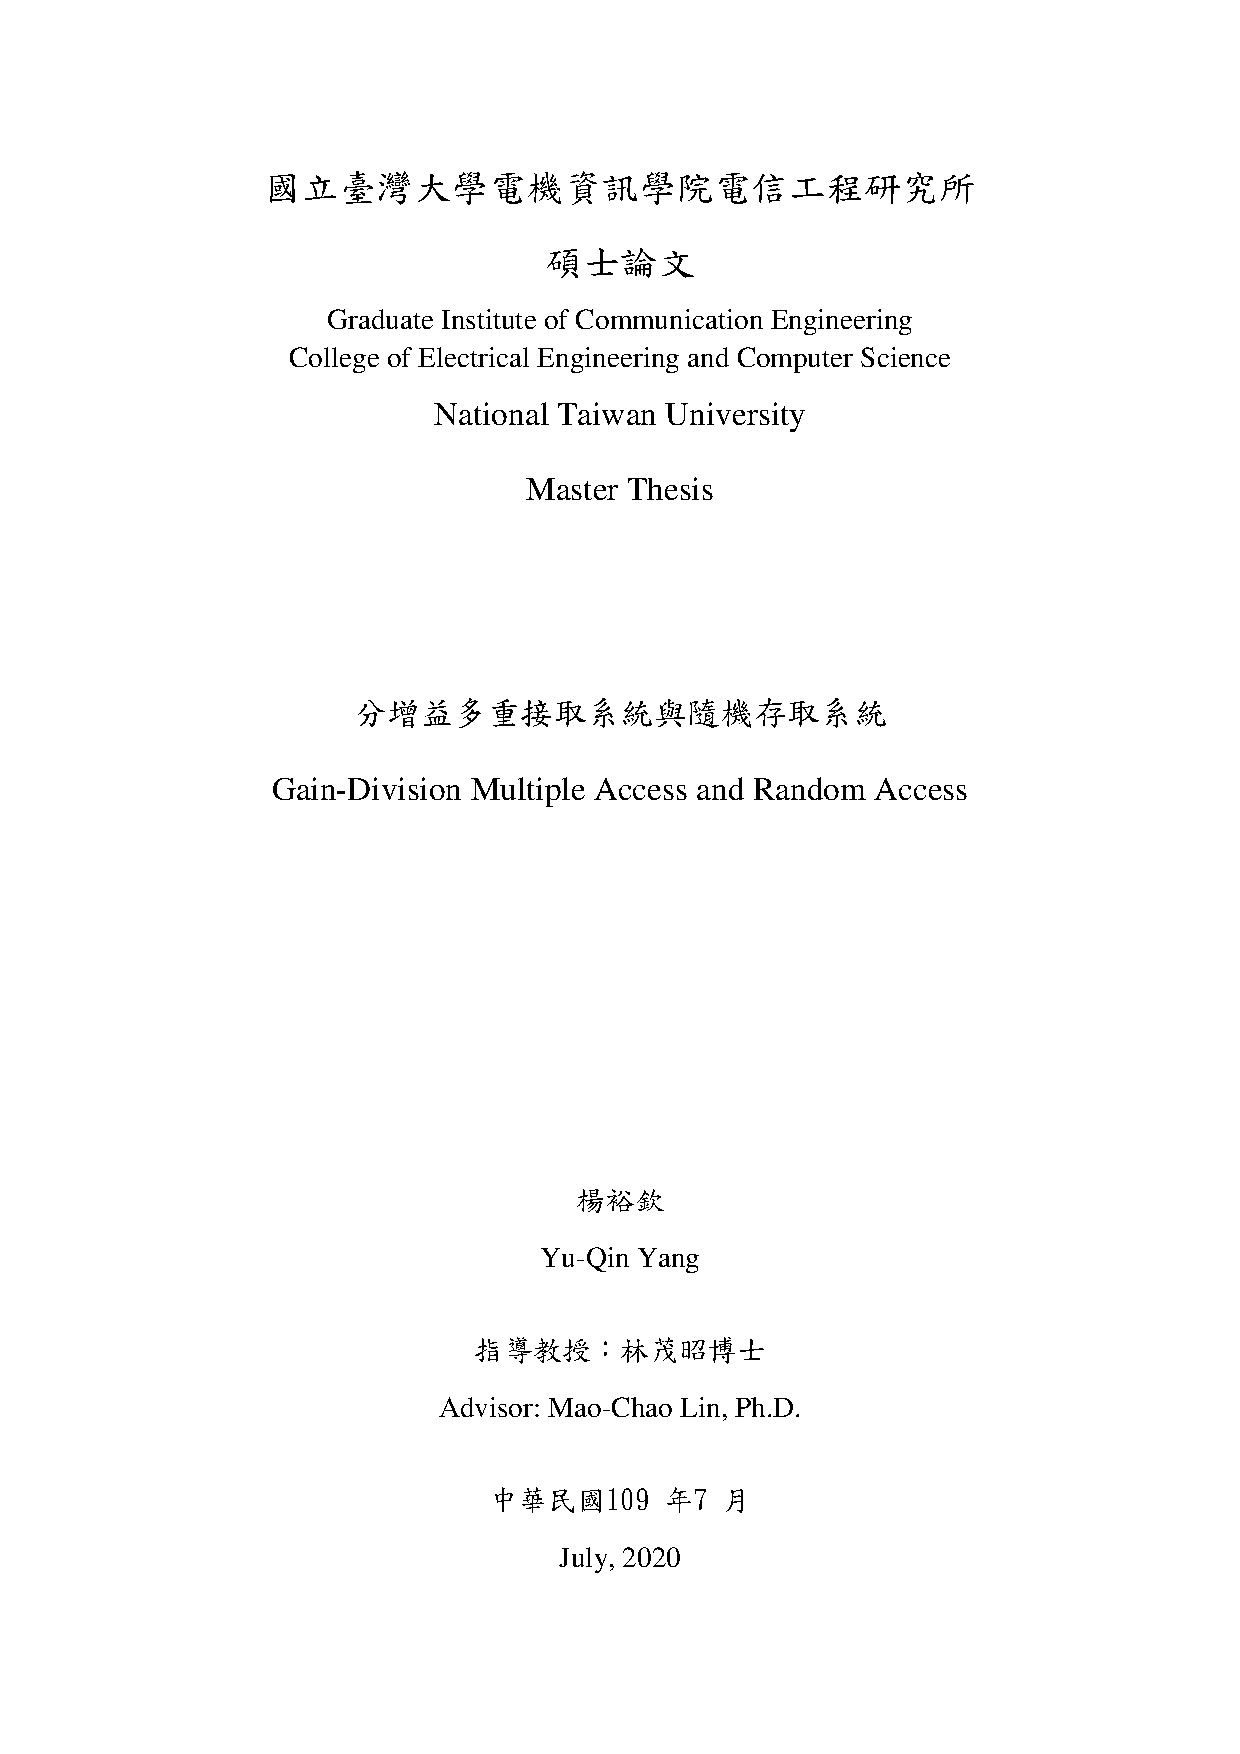
\includepdf[pages={1}]{cover.pdf}

%----------- side page, used for printing on spline -----------
%\makeside

\frontmatter
%----------- generate the certification page by LaTeX -----------
%\makecertification
%----------- includepdf by using package pdfpages -----------
\addcontentsline{toc}{chapter}{口試委員會審定書}
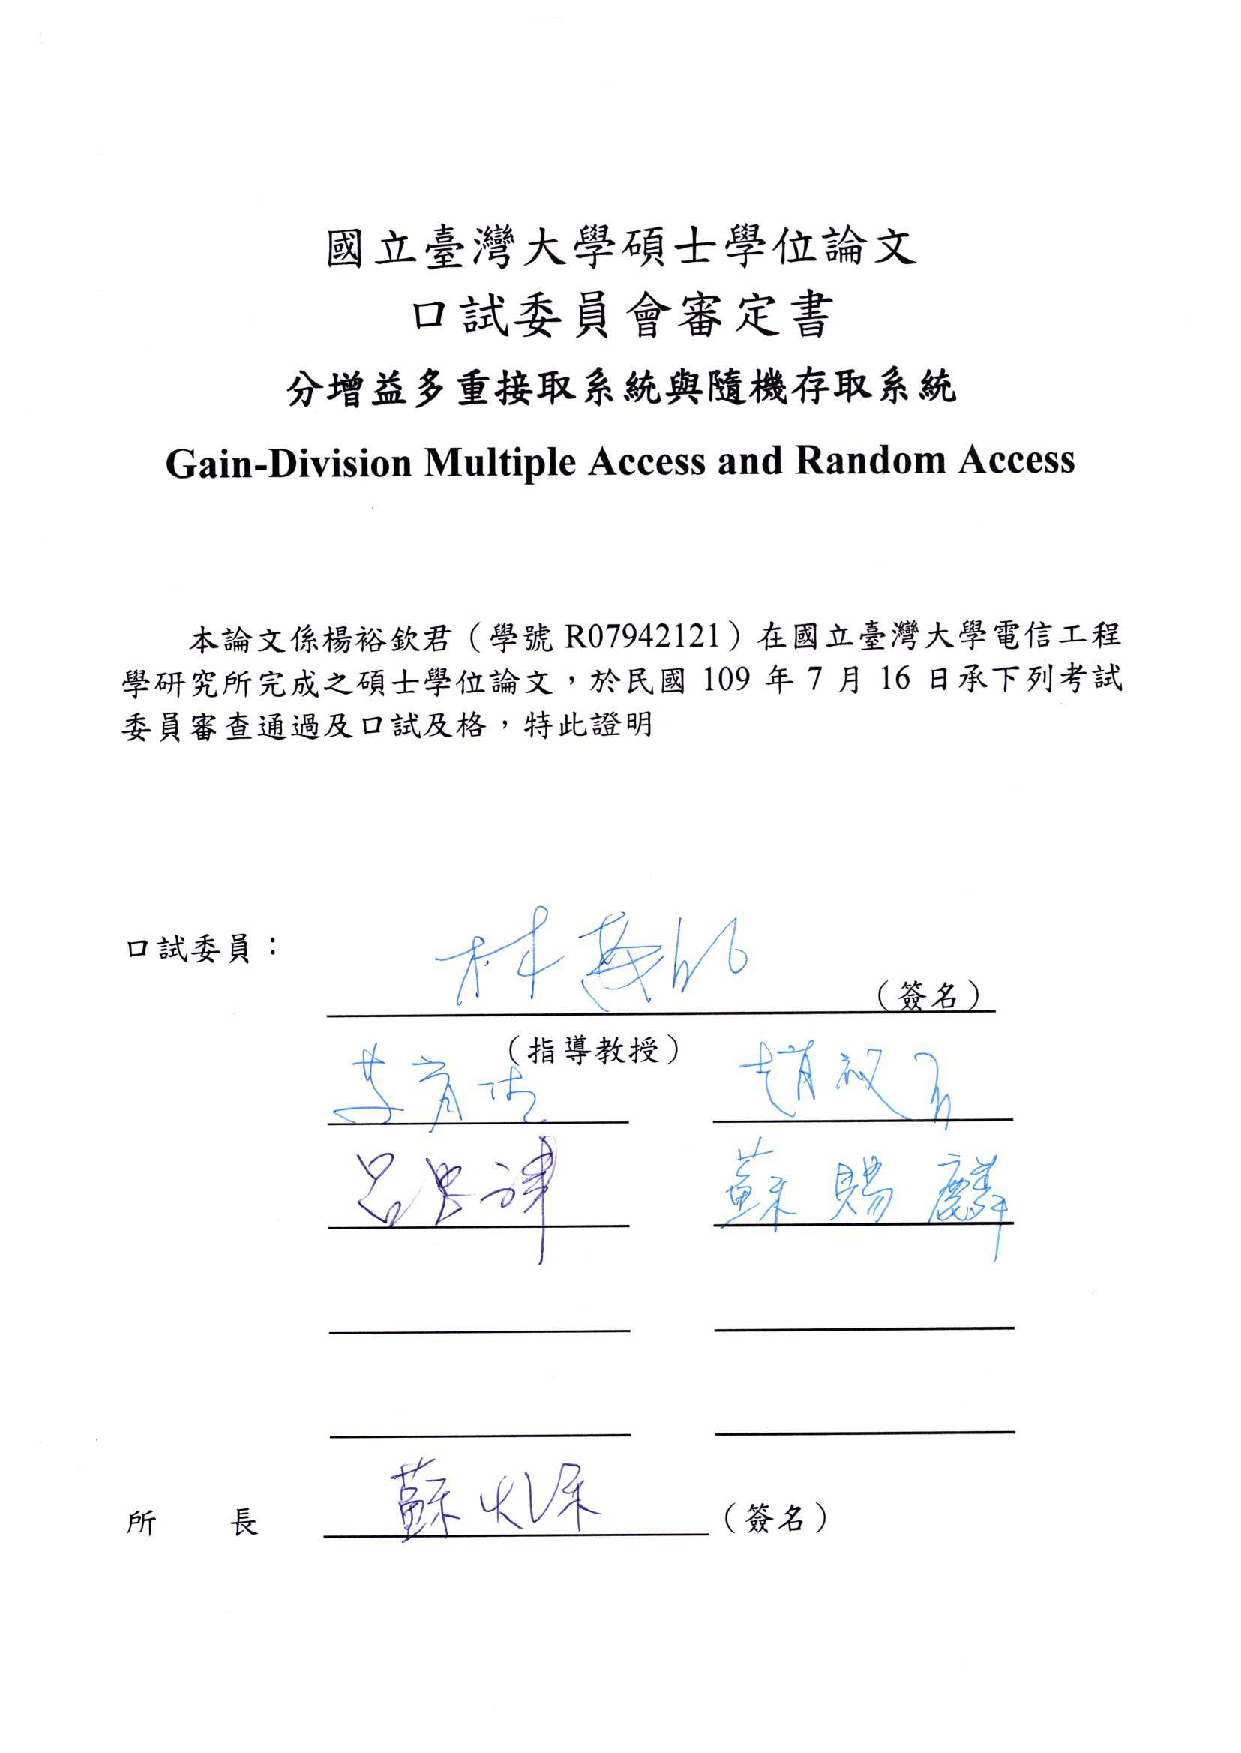
\includepdf[pages={1}]{cert_r07942121.pdf}

\onehalfspacing
\spacing{1.5}
\begin{acknowledgementsCH}

首先要感謝我的指導教授林茂昭教授,在研究部分給我們很大的空間來發揮自己的想像力,時而給我們指點迷津,感謝李世楷教授時而指點我研究的盲點,讓我不會陷入錯誤迴圈,感謝李晃昌教授適時的給予一些幫助。再來也要感謝學長們,感謝會名跟亭宣學長的搞笑為實驗室帶來歡樂,讓實驗室和樂融融,感謝永超跟家俊學長的技術指導讓我受益良多,讓我節省了很多研究時間。接著感謝我的同屆同學,感謝籌尹跟我一起頑皮、感謝得生帶來話題、感謝薏如給我問問題,大家也都不吝嗇給我一些研究上的想法,讓我覺得很感動。再來謝謝我的學弟妹們,柏翰、政晏、律琦,雖然碩二比較少去實驗室,沒有很常看到你們,但是有空可以再辦實驗室活動來聚一聚,最後再次感謝503實驗室的大家。

\end{acknowledgementsCH}
\begin{abstractCH}

分增益多重存取技術是一種最近被提出的多重存取技術,它是利用各個使用者獨立的通道係數來達成多重存取,因此多個使用者可以使用同樣的通道資源同時進行傳送。本篇論文對分增益多重存取技術作進一步研究並研究將其應用於隨機存取系統。

我們提出了分增益多重存取技術的疊加信號與log-likelihood ratio的較通用的表示形式,讓其在實作上更為簡單方便。此外,針對使用極化碼的分增益多重存取,我們也提出了聯合通道解碼方式,讓分增益多重存取技術有更好的效果。

針對先前文獻中基於分群演算法通道盲測之技術,我們也提出了改進方式以取得更接近克拉馬-羅下限的性能。我們也提出了適用於各種星座圖調變以及認意使用者數目來求取通道係數的通用法則。

此外,我們將分增益多重存取技術應用在隨機存取的通道上,利用扎德奧夫-朱序列來進行同步分析和輔助通道估測。性能遠優於不考慮多重存取設計的一般隨機存取。

\

關鍵字:多重接取、衰弱通道、通道估計、盲蔽估測、分群演算法、極化碼、聯合通道解碼、 隨機存取、扎德奧夫-朱序列、同步。

\end{abstractCH}

\begin{abstractEN}

Gain division multiple access (GDMA) is a recently proposed multiple access technique that allows multiple users to share the same resource by exploiting distinct channel coefficients associated with distinct users. In this thesis, we conduct an extended study of GDMA and also its applications to random access.

We propose a general formula for expressing the superimposed signal of all users and the log-likelihood ratio of each user bit.  As to the polar coded GDMA, we propose a joint channel decoder that achieved better BLER performance as compared to the decoding using separate decoders.

In the literature, blind estimation schemes based on the clustering algorithm for the GDMA system were proposed.  In this thesis, we proposed improved methods as that the channel estimation can be closer to the Cramer Rao bound.   In the literature, blind estimation schemes based on the clustering algorithm allow only a small number of users and modulation with small constellation sizes.  We propose a method that can be applied to a random user number and a random constellation. 

\

In the random access techniques, uncoordinated users transmit packets randomly. We introduced a random access system using GDMA.  Zadoff-Chu sequence is used to assist the acquisition of synchronization and channel estimation. The resultant throughput is superior to the conventional random access system ,which fails upon collision without using multiple access.  


\

Key words: Multiple access, fading channel, channel estimation, blind estimation, clustering algorithm, Polar codes, Joint channel  decoder, Radom access, Zadoff-Chu sequence, Synchronization.

\end{abstractEN}


\fontsize{13pt}{19pt}
\selectfont

\tableofcontents

\doublespacing

\listoffigures
\listoftables

\mainmatter

\doublespacing

\fontsize{13pt}{19pt}
\selectfont

%----------- Include/Input your thesis here -----------
%normal cite == \input

\chapter{Introduction}
\label{c:intro}

Multiple access techniques are critical topics in cellular mobile communications. In most of the multiple access systems, users are allowed to transmit signals simultaneously through different types of user-specific signatures. However, the number of users that can be served in a multiple access system is usually limited due to the constraint of user-specific signatures in the allocated resources.  Compared to orthogonal multiple access schemes, non-orthogonal multiple access (NOMA)\cite{shahab2019grant} that allows the overlapping of multiple users over a radio resource can make the resource allocation more flexible.  In \cite{shahab2019grant}, a survey paper, briefly classified NOMA into different types such as the scrambling based Power Domain (PD)
-NOMA, the spreading based SCMA, the interleaving based IDMA.  In \cite{bh18}, a novel multiple access techniques called gain-division multiple access (GDMA) was investigated.  We can define GDMA as a gain-based NOMA system.

Different from PD-NOMA that multiple users are superposed according to the specific power domain, the gain-division multiple access (GDMA) utilizes the different combinations of amplitudes and phase shifts in channel coefficients caused by the independent fading channels. Hence, $U$ users are allowed to share the same transmit resource with multi-level detection in the GDMA system. The detection scheme of GDMA originated from the concept of physical layer network coding (PLNC), which coordinates transmissions among nodes, and packet collisions in traditional wireless networks can be eliminated \cite{plnc06}. 

In forward error coding GDMA system, there are two types of detection principles: separate channel decoding (SCD) and joint channel decoding (JCD). GDMA-SCD is a straightforward method that separates individual information from superimposed signal information, and there is no exchange of information between collided users. GDMA-JCD is a more sophisticated method that employs all information of superimposed signals to decode. In \cite{yt19}, a joint channel decoding and physical-layer network coding (G-JCNC)\cite{gjcnc10} was applied for the GDMA LDPC coded system. However, there is no effective JCD for polar code. We introduced JCD decoders for a polar coded system, which can effectively improve the error performances. 

Since the multiuser detection technique (MUD) in the GDMA system allows $U$ users to share the same resource, each of the received symbols consisting of the signals transmitted from $U$ users can be seen as a superimposed signal with $2^{mU}$ levels where $m$ is the modulation order. A blind channel estimation scheme\cite{yt19} was proposed for achieving spectral efficiency since no additional pilot signal is needed for channel estimation. Firstly, the system classifies the received symbols into $2^{mU}$ groups by applying a clustering algorithms\cite{lbg80}\cite{kmpp07}\cite{em77}, where the symbols corresponding to the same superimposed level are grouped together, the estimates of the levels can be attained through the average of the symbols in each group. Secondly, the system utilizes the geometrical configuration of clustering estimated $2^{mU}$ levels to derive an estimated $U$ channel gains. Thirdly, a phase ambiguity algorithm is used to remove the phase ambiguity. 
  
In this thesis, we proposed a general adaptive clustering algorithm that can reduce the complexity and achieve Mean Square Error (MSE) for channel estimation closer to the Cramer Rao (CR) bound as compared to the algorithm used in \cite{yt19}.  In \cite{yt19}, the algorithm for the first and second stages can only be applied for a small amount of users $U$ and for modulation with small order $m$. With this observation, we also propose an algorithm for deriving channel gains by recursive operations. This algorithm can be applied to any number $U$ of users and any constellation size $m$.

Recently, random access (RA) protocols have acquired a lot of attention, not only from satellite communication but also from researchers active in fields such as Internet of Things (IoT) and machine-to-machine communications. Random access is a multiuser communication system in which users transmit packets over a shared channel, which is random. When there is more than one packets in the time duration, these packets collide, which results in transmission failure. Based on the conventional RA scheme (ALOHA system), several random access protocols were developed.  Most of them used more channel resources to avoid collisions.  To tackle the condition for which there are many device connections and few channel resources, we introduce a novel RA scheme which resolves the collisions without additional channel resources by applying the GDMA concept. The scenarios of slotted, un-slotted, grant-based, and grant-free for the RA-GMDA system are investigated. The preamble signals are used for synchronization and channel estimation, where the preamble based channel estimation can be integrated into the clustering based channel estimation. 


The organization of this thesis is as follows. In Chapter~\ref{c:gdma}, basic concepts of the GDMA technique are reviewed ,and the system models are also illustrated. The modified cluster-based channel estimation for the GDMA system is proposed in Chapter~\ref{c:cluster_ce} including the clustering algorithms and the schemes to resolve the phase ambiguity problem. Moreover, the GDMA based random access scheme is proposed in Chapter~\ref{c:rach_gdma}. Concluding remarks and future works are presented in Chapter~\ref{c:remarks}.

\chapter{Gain-Division Multiple Access}
\label{c:gdma}

In this chapter, we consider the scenario for uplink transmissions over independent fading channels, and the gain-division multiple access (GDMA) with a multiuser detection technique is reviewed for further discussions.

%==================================================

\section{Detection Principle}

A communication system in which $U$ users are sharing the same transmit resource is considered, and the symbol timings of transmissions are assumed to be perfectly aligned. The block diagram of transmitters is shown in Fig.~\ref{fig:gdma_tx}. The message bit sequence ${\bf{d}}_p = [d_u(1), d_u(2), ..., d_u(k)]$ of user-$u$ is encoded into the codeword ${\bf{c}}_u = [c_u(1), c_u(2), ..., c_u(N_c)]$ by an $(N_c,k)$ forward error-correction (FEC) code with code rate $k/N_c$, and the codeword ${\bf{c}}_p$ is then passed to the modulator with order $m$ to get the sequence of modulated symbols ${\bf x}_p = [x_u(1), x_u(2), ..., x_u(N_c/m)]$. The signals of $U$ users are transmitted to the receiver through the independent Rayleigh flat-fading channels, and each of the received symbols in sequence ${\bf r} = [r(1), r(2), ..., r(N_c/m)]$ can be represented as
\begin{align} \label{equ:rx_sup}
 r(n) &= \sum_{u=1}^{U}h_{u}x_{u}(n) + w(n) \nonumber \\ &= s(n) + w(n) ,
\end{align}
where $h_u$ is the channel coefficient between user-$u$ and the receiver, $w(n)$ is the complex additive white Gaussian noise (AWGN) and $s(n)$ is the superimposed symbol consisting of the signals transmitted from $U$ users. There are $2^{mU}$ possible levels in each $s$, where we drop the symbol index $n$ for brevity, and the levels are distinguishable due to the effect of independent fading channels. 

\begin{figure}[t!]
 \centering
 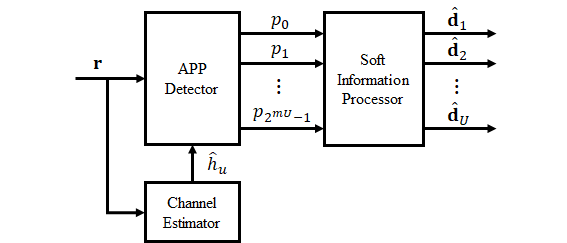
\includegraphics[width=15cm]{fig/gdma_tx.png}
 \caption{Transmitters of $U$ users occupying the same resource.}
 \label{fig:gdma_tx}
\end{figure}

The channel coefficient $h_u$ for a Rician distributed channel can be represented as
\begin{align} \label{equ:rx_sup}
 h_{u} &=\frac{1}{\sqrt{K+1}} \cdot a+\frac{\sqrt{K}}{\sqrt{K+1}}\cdot b \cdot i,
\end{align}

where $a$ and $b$ are normal distribution with variance 1, $a$ is the real part coefficient and $b$ is the imaginary part. $h_{u}$ is the Rayleigh distribution for $K=0$, and Racian distribution for $K\ne0$.


 \begin{figure}[H]
 \centering
 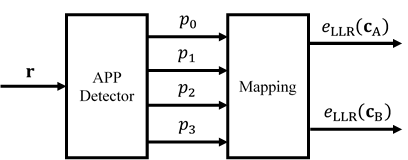
\includegraphics[width=12cm]{fig/gdma_bpsk_u2.png}
 \caption{GDMA detecter for BPSK and $U=2$.}
 \label{fig:gdma_bpsk_u2}
\end{figure}

For the GDMA detector, we divided it into two steps to illustrate.  Firstly, we obtained a $2^{mU}$ dimension probability vector of $a \ posteriori$ probabilities (APPs) for all the superimposed signals. Secondly, Map the $2^{mU}$ dimension probability vector into $U$ Log-likelihood Ratio(LLR). Fig.~\ref{fig:gdma_bpsk_u2} is the block diagram of the GDMA detector in the case of $U = 2$ and BPSK modulation ($m=1$), and the users are denoted as user-A and user-B. The mapping rules for code bits of two users and superimposed levels are tabulated in Table~\ref{table:mapping_m1_p2}, and the possible levels of $s$ are denoted as $S[l]$ with $l \in \{0, 1, 2, 3\}$. In Fig.~\ref{fig:constellation_m1_p2}, a graphical example of the superimposed levels and the corresponding binary mappings $(c_\text{A}, c_\text{B})$ is provided when $h_{\text{A}}$ and $h_{\text{B}}$ are the channel coefficients of user-A and user-B respectively. Note that an accurate estimation of channel coefficients for all users is necessary to recognize the superimposed signal levels properly. In this chapter, we assume that the channel state information (CSI) can be perfectly recovered at the receiver. Thus we can derive all the possible levels of received symbol $s$ for further detection.  

\begin{table}[t!]
\caption{Mapping rules for superimposed signal in the case of $m=1$ and $U=2$.}
\begin{center}
\extrarowheight=2.5pt
\begin{tabular}{|>{\centering\arraybackslash}m{\columnwidth/15}||>{\centering\arraybackslash}m{\columnwidth/10}|>{\centering\arraybackslash}m{\columnwidth/10}||>{\centering\arraybackslash}m{\columnwidth/10}|>{\centering\arraybackslash}m{\columnwidth/10}||>{\centering\arraybackslash}m{\columnwidth/7}|}
\hline 
 $l$ & $c_\text{A}$ & $c_\text{B}$ & $x_\text{A}$ & $x_\text{B}$ &           $S[l]$         \\ \hline
  0  &      0       &      0       &      1       &      1       & $ h_\text{A}+h_\text{B}$ \\ \hline 
  1  &      0       &      1       &      1       &     -1       & $ h_\text{A}-h_\text{B}$ \\ \hline 
  2  &      1       &      0       &     -1       &      1       & $-h_\text{A}+h_\text{B}$ \\ \hline 
  3  &      1       &      1       &     -1       &     -1       & $-h_\text{A}-h_\text{B}$ \\ \hline
\end{tabular}
\label{table:mapping_m1_p2}
\end{center}
\end{table}

\begin{figure}[t!]
 \centering
 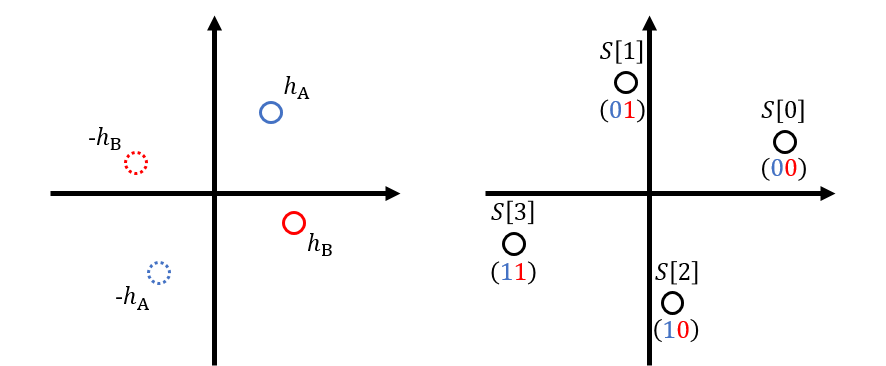
\includegraphics[width=15cm]{fig/constellation_m1_p2.png}
 \caption{An example of superimposed levels in the case of $m=1$ and $U=2$.}
 \label{fig:constellation_m1_p2}
\end{figure}

The $a \ posteriori$ probabilities (APPs) that $s$ is the $l$-th level with $l \in \{0,1,2,3\}$ given the received symbol $r$ can be calculated by
\begin{align}
 p_{l} &= \text{Pr}\left\{s = S[l]\middle|r\right\} \nonumber \\
	   &= \text{Pr}\left\{r\middle|s = S[l]\right\}\cdot\frac{\text{Pr}\left\{s = S[l]\right\}}{\text{Pr}\left\{r\right\}} ,
\label{equ:app} 
\end{align}
and

\begin{align}
 \text{Pr}\left\{r\middle|s = S[l]\right\} = \frac{1}{2\pi{\sigma_w}^{2}}\exp\left(-\frac{\lvert r-S[l]\rvert^{2}}{2{\sigma_w}^{2}}\right) ,
\label{equ:app_2}
\end{align}

where $\text{Pr}\{s = S[l]\}$ is the $a \ priori$ probabilities of $s$ and ${\sigma_w}^2$ is the variance of AWGN. According to the concept of physical layer network coding (PLNC), the APPs of code bits given the received symbol $r$ can be obtained as
\begin{align}
 \text{Pr}\left\{c_\text{A} = 0 \middle| r\right\} &= \text{Pr}\left\{s = S[0]\middle|r\right\} + \text{Pr}\left\{s = S[1]\middle|r\right\} = p_{0} + p_{1}, \nonumber \\
 \text{Pr}\left\{c_\text{A} = 1 \middle| r\right\} &= \text{Pr}\left\{s = S[2]\middle|r\right\} + \text{Pr}\left\{s = S[3]\middle|r\right\} = p_{2} + p_{3},
\end{align}
and
\begin{align}
 \text{Pr}\left\{c_\text{B} = 0 \middle| r\right\} &= \text{Pr}\left\{s = S[0]\middle|r\right\} + \text{Pr}\left\{s = S[2]\middle|r\right\} = p_{0} + p_{2}, \nonumber \\
 \text{Pr}\left\{c_\text{B} = 1 \middle| r\right\} &= \text{Pr}\left\{s = S[1]\middle|r\right\} + \text{Pr}\left\{s = S[3]\middle|r\right\} = p_{1} + p_{3}.
\end{align}

The APPs of code bits can be derived for multiple users with the observation of received superimposed symbols as long as the CSI is available at the receiver. Once the APPs of code bits are obtained, the corresponding log-likelihood ratios (LLRs) of code bits are given by
\begin{align}
 e_{\text{LLR}}(c_\text{A}) = \ln \frac {\text{Pr}\{c_\text{A} = 0|r\}} {\text{Pr}\{c_\text{A} = 1|r\}} = \ln\frac {p_{0}+p_{1}} {p_{2}+p_{3}}, \nonumber \\
 e_{\text{LLR}}(c_\text{B}) = \ln \frac {\text{Pr}\{c_\text{B} = 0|r\}} {\text{Pr}\{c_\text{B} = 1|r\}} = \ln\frac {p_{0}+p_{2}} {p_{1}+p_{3}}.
\label{equ:bit_mapping}
\end{align}


\begin{table}[H]
\caption{Mapping rules for superimposed signal in the case of $m=1$ and $U=3$.}
\begin{center}
\extrarowheight=2pt
\begin{tabular}{|>{\centering\arraybackslash}m{\columnwidth/22}||>{\centering\arraybackslash}m{\columnwidth/14}|>{\centering\arraybackslash}m{\columnwidth/14}|>{\centering\arraybackslash}m{\columnwidth/14}||>{\centering\arraybackslash}m{\columnwidth/14}|>{\centering\arraybackslash}m{\columnwidth/14}|>{\centering\arraybackslash}m{\columnwidth/14}||>{\centering\arraybackslash}m{\columnwidth/5}|}
\hline
 $l$ & $c_1$ & $c_2$ & $c_3$ & $x_1$ & $x_2$ & $x_3$ &     $S[l]$     \\ \hline
  0  &   0   &   0   &   0   &   1   &   1   &   1   & $ h_1+h_2+h_3$ \\ \hline 
  1  &   0   &   0   &   1   &   1   &   1   &  -1   & $ h_1+h_2-h_3$ \\ \hline 
  2  &   0   &   1   &   0   &   1   &  -1   &   1   & $ h_1-h_2+h_3$ \\ \hline 
  3  &   0   &   1   &   1   &   1   &  -1   &  -1   & $ h_1-h_2-h_3$ \\ \hline
  4  &   1   &   0   &   0   &  -1   &   1   &   1   & $-h_1+h_2+h_3$ \\ \hline 
  5  &   1   &   0   &   1   &  -1   &   1   &  -1   & $-h_1+h_2-h_3$ \\ \hline 
  6  &   1   &   1   &   0   &  -1   &  -1   &   1   & $-h_1-h_2+h_3$ \\ \hline 
  7  &   1   &   1   &   1   &  -1   &  -1   &  -1   & $-h_1-h_2-h_3$ \\ \hline
\end{tabular}
\label{table:mapping_m1_p3}
\end{center}
\end{table}

\begin{figure}[t!]
 \centering
 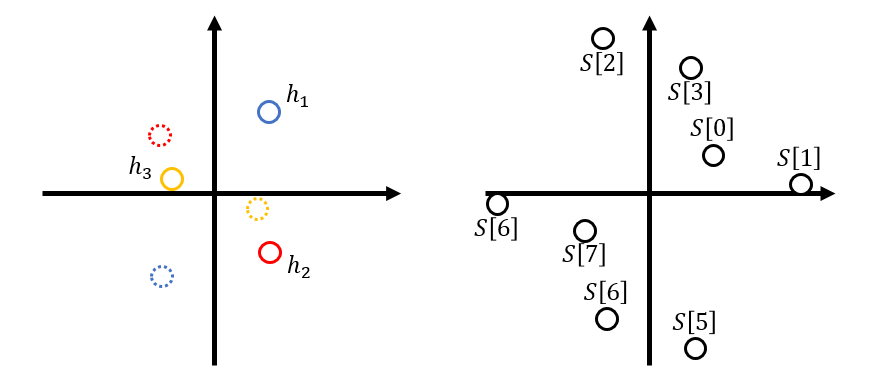
\includegraphics[width=15cm]{fig/constellation_m1_p3.png}
 \caption{An example of superimposed levels in the case of $m=1$ and $U=3$.}
 \label{fig:constellation_m1_p3}
\end{figure}

The multi-level detection technique in GDMA system can be easily extended to the system with $U>2$ and/or $m>1$. For example, in the case of $m=1$ and $U=3$, the mapping rules for code bits of users, denoted as user-1, user-2 and user-3, and superimposed levels are tabulated in Table~\ref{table:mapping_m1_p3}. There are eight possible levels in each superimposed symbol $s$. Let $p_l$ with $l \in \{0,1,...,7\}$ denote the APPs of $s$ given in (\ref{equ:app}), the LLRs of code bits are
\begin{align}
 e_{\text{LLR}}({c}_1) = \ln \frac {\text{Pr}\{c_1 = 0|r\}} {\text{Pr}\{c_1 = 1|r\}} = \ln\frac {p_{0}+p_{1}+p_{2}+p_{3}} {p_{4}+p_{5}+p_{6}+p_{7}}, \nonumber \\
 e_{\text{LLR}}({c}_2) = \ln \frac {\text{Pr}\{c_2 = 0|r\}} {\text{Pr}\{c_2 = 1|r\}} = \ln\frac {p_{0}+p_{1}+p_{4}+p_{5}} {p_{2}+p_{3}+p_{6}+p_{7}}, \nonumber \\
 e_{\text{LLR}}({c}_3) = \ln \frac {\text{Pr}\{c_3 = 0|r\}} {\text{Pr}\{c_3 = 1|r\}} = \ln\frac {p_{0}+p_{2}+p_{4}+p_{6}} {p_{1}+p_{3}+p_{5}+p_{7}}.
\label{equ:p3_llr}
\end{align}


%==================================================

\section{Implementation Methood}

Although the concept of GDMA detection is straightforward, there is no general method to implement the GDMA detector \cite{bh18}\cite{yt19} ,which establishes a mapping table for a specific $U$. With the rise of $U$, the mapping table will grow exponentially, which will significantly improve the complexity of GDMA, and it is challenging to implement. Therefore, we propose a general method that can be implemented more simply and efficiently in this chapter.

\subsection{BPSK-modulated GDMA Implementation}

For general express for BPSK GDMA, we divide the detection into three steps: definition of levels, derivation of APPs ,and derivation of LLRs. Firstly, the superimposed signals $S[l],l\in{1,2,\cdots,L}$ can be express as

\begin{align}
S[1] &= h_{1} + h_{2} + \cdots + h_{U}&={(-1)}^{0} \cdot h_{1}+{(-1)}^{0} \cdot h_{2}+ \cdots + {(-1)}^{0} \cdot h_{U},
 \nonumber \\
S[2] &= h_{1} + h_{2} + \cdots - h_{U}&={(-1)}^{0} \cdot h_{1}+{(-1)}^{0} \cdot h_{2}+ \cdots + {(-1)}^{1} \cdot h_{U}, 
\nonumber \\
\vdots 
\nonumber \\
S[L] &= - h_{1} - h_{2} - \cdots - h_{U}&={(-1)}^{1} \cdot h_{1}+{(-1)}^{1} \cdot h_{2}+ \cdots + {(-1)}^{1} \cdot h_{U}.
\nonumber \\
\end{align}

Convert the decimal $l_{10}$ into binary $l_{2}$, and define $l_{2}$[$u$] is the $u$ -th bit of binary $l_{2}$.  $l_{10} = l_{2} = (l_{2}[1] \quad l_{2}[2] \quad \cdots \quad l_{2}[U])$, $u=1,2,\cdots,U, l_{10} = 0, \cdots, L-1$. We consider that $l_{10}$ is the serial number to record superimposed levels and consider that $l_2[u]$ is the code bit for user-$u$. Moreover, $l_2[u]$ is also a mapping index for $u$-user's channel gain $h_u$. We can derive mapping index from $S[l]$ directly by converting from decimal to binary. In the following expression, $l_{10}$ and $l_2$ are used alternately.

\begin{align}
S[l_{10}] &={(-1)}^{l_{2}[1]} \cdot h_{1}+{(-1)}^{l_{2}[U]} \cdot h_{2}+ \cdots + {(-1)}^{l_{2}[U]} \cdot h_{U} 
\nonumber \\
&= \sum_{u=1}^{U} (-1)^{l_2[u]} \cdot h_u, l_{10} = 0, 1, \cdots, L-1 
\label{equ:implementation_1}
\end{align}
where $h_{u}$ is the complex channel coefficient of user-$u$. Secondly, APPs of $l$-th level with $l\in{0,1,2,\cdots,L}$ given the received symbol $r$ can be calculated as equation.\ref{equ:app}. Thirdly, once the APPs are obtained, the mapping formula can be expressed as 

\begin{align}
e_{\text{LLR}}[c_u] &= ln \frac{\text{Pr}\{c_u=0|r\}}{\text{Pr}\{c_u=1|r\}}
\nonumber \\
&= ln \frac{\sum_{l_{10}=0, l_{2}[u]\in{0}}^{L}\text{Pr}\{s=S[l]|r\}}{\sum_{l_{10}=0, l_{2}[u]\in{1}}^{L}\text{Pr}\{s=S[l]|r\}}
\label{equ:implementation_2}
\end{align}

\begin{figure}[b!]
 \centering
 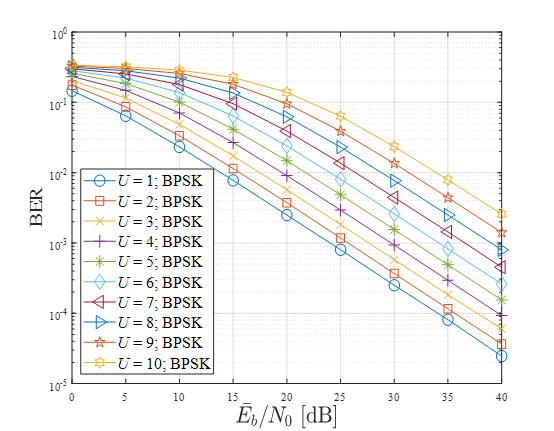
\includegraphics[width=15cm]{fig/gdma_bpsk_implement_u2.png}
 \caption{BER performances of uncoded GDMA BPSK system over block Rayleigh fading channels.}
 \label{fig:bpsk_implementation}
\end{figure}

The two equations above and below the fraction are the probability that user-$u$ code bits are equal to zero or one, and there are $\frac{L}{2}$ APPs added respectively. The APPs of the upper fraction must meet $h_u$ superimposition, and the APPs of the lower fraction must meet $-h_u$ superimposition. According to \ref{equ:implementation_1}, we can use mapping index $l_2[u]$ equal to zero or one to judge whether meet the $u$-user restriction.



\subsection{QPSK-modulated GDMA Implementation}

 In addition to BPSK, we also discuss the general detection of QPSK with modulation order ($m=2$). According to QPSK modulation, the superimposed signals $S[l],l\in{1,2,\cdots,L}$ can be expressed as
\begin{align}
S[0] &= e^{\frac{\pi}{4}j}h_{1} + e^{\frac{\pi}{4}j}h_{2} + \cdots + e^{\frac{\pi}{4}j}h_{U},
\nonumber \\
S[1] &= e^{\frac{\pi}{4}j}h_{1} + e^{\frac{\pi}{4}j}h_{2} + \cdots + e^{(\frac{\pi}{4}+\frac{\pi}{2})j}h_{U},
\nonumber \\
S[2] &= e^{\frac{\pi}{4}j}h_{1} + e^{\frac{\pi}{4}j}h_{2} + \cdots + e^{(\frac{\pi}{4}+\pi)j}h_{U},
\nonumber \\
S[3] &= e^{\frac{\pi}{4}j}h_{1} + e^{\frac{\pi}{4}j}h_{2} + \cdots + e^{(\frac{\pi}{4}+\frac{3\pi}{2})j}h_{U},
\nonumber \\
\vdots 
\nonumber \\ \nonumber \\
S[L-1] &= e^{(\frac{\pi}{4}+\frac{3\pi}{2})j}h_{1} + e^{(\frac{\pi}{4}+\frac{3\pi}{2})j}h_{2} + \cdots + e^{(\frac{\pi}{4}+\frac{3\pi}{2})j}h_{U}.
\label{equ:implementation_4}
\end{align}

Different from BPSK detection, we convert the decimal $l_{10}$ into quaternary $l_{4}$ since the modulation order $(m=2)$, and define that $l_{4}[u]$ is the $u$-th bit of quaternary $l_{4}$. $l_{10}=l_{4}=(l_4[1]  \quad l_4[2] \quad  \cdots \quad  l_4[U]),u=1,2,\cdots U$.  We consider that $l_4[u]$ is the code symbol for user-$u$, which might be 00, 01, 10, 11. Moreover, $l_4[u]$ is also a mapping index for $u$-user's channel gain $h_u$. After simplifying \ref{equ:implementation_4}, we can obtain superimposed levels as

\begin{align}
S[l] &= e^{(\frac{\pi}{4} + \frac{\pi}{2} \cdot l_{4}[1])j} \cdot h_{1} + e^{(\frac{\pi}{4} + \frac{\pi}{2} \cdot l_{4}[1])j} \cdot h_{2} + \cdots + e^{(\frac{\pi}{4} + \frac{\pi}{2} \cdot l_{4}[1])j} \cdot h_{U} 
\nonumber \\
&= \sum_{u=1}^{U}e^{(\frac{\pi}{4} + \frac{\pi}{2} \cdot l_{4}[u])j} \cdot h_{u}, l_{10}= 0, 1, \cdots, L-1; u=1, 2, \cdots, U
\label{equ:qpsk_level_define}
\end{align}

In the above definition \ref{equ:qpsk_level_define}, we can define levels architecturally, and then need to derive the APP of each level. The 
APPs can be calculated as \ref{equ:app}. Finally,  $e_{\text{LLR}}$ can be easily obtained with the structure of $S[l]$.

\begin{equation}
e_{\text{LLR}}[c_u] = ln \frac{\text{Pr}\{c_u=0|r\}}{\text{Pr}\{c_u=1|r\}} 
\nonumber \\ = 
\left\{
             \begin{array}{lr}
             ln \frac{\sum_{l_{10}=0, l_{2}[u]\in\{0,1\}}^{L}\text{Pr}\{s=S[l]|r\}}{\sum_{l_{10}=0, l_{2}[u]\in\{2,3\}}^{L}\text{Pr}\{s=S[l]|r\}}, i = 1; u=1,\cdots, U &  \\
             ln \frac{\sum_{l_{10}=0, l_{2}[u]\in\{0,2\}}^{L}\text{Pr}\{s=S[l]|r\}}{\sum_{l_{10}=0, l_{2}[u]\in\{1,3\}}^{L}\text{Pr}\{s=S[l]|r\}},
i = 2; u=1,\cdots, U & \\ 
             \end{array}
\right.
\label{equ:implementation_3}
\end{equation}

	The Fig.\ref{fig:qpsk_gray_mapping} is the QPSK constellation according to gray mapping. We need to consider the code bit code bits corresponding to the first or the second bit on constellation. For first bit $i=1$, both level-$S[0]$ and level-$S[1]$ are mapping to code bit equal to $0$, while level-$S[2]$ and level-$S[3]$ are mapping to code bits equal to $1$, where $i=1,\cdots, m$ is the $i$-bit for constellation. We also can use mapping index $l_{4}[u]$ to extract the phase information from $S[l]$. Map LLR according to $i$-constellation location and $u$-user. 
	
	Fig.\ref{fig:qpsk_implementation} is the BER performance of uncoded GDMA QPSK over a block rayleigh fading channel.

\begin{figure}
 \centering
 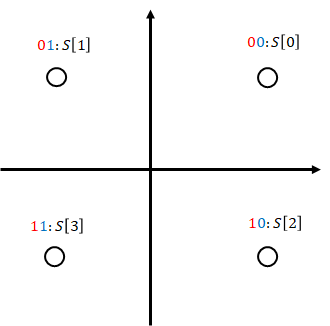
\includegraphics[width=7cm]{fig/qpsk_gray_mapping.png}
 \caption{QPSK modulation gray mapping.}
 \label{fig:qpsk_gray_mapping}
\end{figure}

\begin{figure}[H]
 \centering
 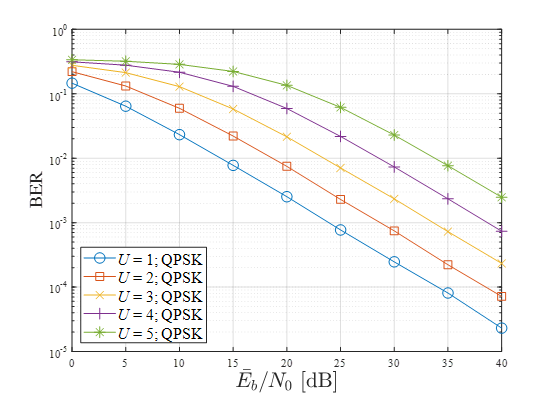
\includegraphics[width=15cm]{fig/gdma_qpsk_implement.png}
 \caption{BER performances of uncoded GDMA QPSK system over block Rayleigh fading channels.}
 \label{fig:qpsk_implementation}
\end{figure}

\subsection{PAM-modulated GDMA Implementation}

Consider a general PAM case: $2^m$-PAM; $U$ is integer; $m$ is integer; $E_v$  is the average power; $M=2^m-1$ is the mid number.

The superimposed signals $S[l],l\in{1,2,\cdots,L}$ can be express as
\begin{align}
S[0] &= (2 \cdot 0-M)\cdot\sqrt{E_s}\cdot h_1 + (2\cdot0 - M)\cdot\sqrt{E_s}\cdot h_2 +, \cdots + (2 \cdot 0-M)\cdot\sqrt{E_s}\cdot h_U,
\nonumber \\
S[1] &= (2 \cdot 0-M)\cdot\sqrt{E_s}\cdot h_1 + (2\cdot0 - M)\cdot\sqrt{E_s}\cdot h_2 +, \cdots + (2 \cdot 1-M)\cdot\sqrt{E_s}\cdot h_U,
\nonumber \\
S[2] &= (2 \cdot 0-M)\cdot\sqrt{E_s}\cdot h_1 + (2\cdot0 - M)\cdot\sqrt{E_s}\cdot h_2 +, \cdots + (2 \cdot 2-M)\cdot\sqrt{E_s}\cdot h_U,
\nonumber \\
S[3] &= (2 \cdot 0-M)\cdot\sqrt{E_s}\cdot h_1 + (2\cdot0 - M)\cdot\sqrt{E_s}\cdot h_2 +, \cdots + (2 \cdot 3-M)\cdot\sqrt{E_s}\cdot h_U,
\nonumber \\
\vdots 
\nonumber \\ 
S[L-1] &= (2 \cdot M-M)\cdot\sqrt{E_s}\cdot h_1 + (2\cdot M - M)\cdot\sqrt{E_s}\cdot h_2 +, \cdots + (2 \cdot M-M)\cdot\sqrt{E_s}\cdot h_U.
\label{equ:implementation_5}
\end{align}

We can convert the decimal $l_{10}$ into quaternary $l_{M}$, and define that $l_{M}[u]$ is the $u$-th bit of $l_{M}$. $l_{10}=l_{M}=(l_M[1]  \quad l_M[2] \quad  \cdots \quad  l_M[U]),u=1,2,…U$. After simplifying \ref{equ:implementation_5}, we can obtain superimposed levels as

\begin{align}
S[l] &= (2 \cdot l_{2^{m}}[1]-M)\cdot\sqrt{E_v}\cdot h_1 + (2 \cdot l_{2^{m}}[2]-M)\cdot\sqrt{E_v}\cdot h_2 +, \cdots + (2 \cdot l_{2^{m}}[U]-M)\cdot\sqrt{E_v}\cdot h_U
\nonumber \\
&= \sum_{u=1}^{U}(2\cdot l_{2^{m}}[u]-M)\cdot\sqrt{E_{v}}\cdot h_u, u=1,2, \cdots, U
\end{align}

In the above definition, we can define levels architecturally and then need to derive the APP of each level. The APPs can be calculated as \ref{equ:app}. Finally,  $e_{\text{LLR}}$ can be easily obtained with the structure of $S[l]$. According to m, there will be different gray mapping for PAM. Firstly, we discuss the 4-PAM and the gray mapping in Fig.\ref{fig:4_pam_gray_mapping}. 

\begin{figure}
 \centering
 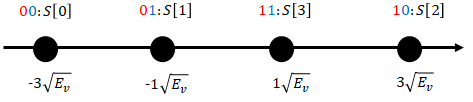
\includegraphics[width=10cm]{fig/4_pam_gray_mapping.png}
 \caption{4-PAM modulation gray mapping.}
 \label{fig:4_pam_gray_mapping}
\end{figure}

\begin{equation}
e_{\text{LLR}}[c_u] = ln \frac{\text{Pr}\{c_u=0|r\}}{\text{Pr}\{c_u=1|r\}} 
\nonumber \\ = 
\left\{
             \begin{array}{lr}
             ln \frac{\sum_{l_{10}=0, l_{4}[u]\in\{0,1\}}^{L}\text{Pr}\{s=S[l]|r\}}{\sum_{l_{10}=0, l_{4}[u]\in\{2,3\}}^{L}\text{Pr}\{s=S[l]|r\}}, i = 1; u=1,\cdots, U &  \\
             ln \frac{\sum_{l_{10}=0, l_{4}[u]\in\{0,3\}}^{L}\text{Pr}\{s=S[l]|r\}}{\sum_{l_{10}=0, l_{4}[u]\in\{1,2\}}^{L}\text{Pr}\{s=S[l]|r\}},
i = 2; u=1,\cdots, U & \\ 
             \end{array}
\right.
\end{equation}

Secondly, we discuss the 8-PAM and the gray mapping \ref{fig:8_pam_gray_mapping}. 

\begin{figure}
\centering
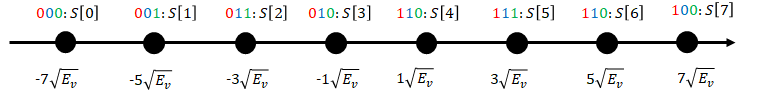
\includegraphics[width=17cm]{fig/8_pam_gray_mapping.png}
\caption{8-PAM modulation gray mapping.}
\label{fig:8_pam_gray_mapping}
\end{figure}

\begin{equation}
e_{\text{LLR}}[c_u] = ln \frac{\text{Pr}\{c_u=0|r\}}{\text{Pr}\{c_u=1|r\}} 
\nonumber \\ = 
\left\{
             \begin{array}{lr}
             ln \frac{\sum_{l_{10}=0, l_{8}[u]\in\{0,1,2,3\}}^{L}\text{Pr}\{s=S[l]|r\}}{\sum_{l_{10}=0, l_{8}[u]\in\{4,5,6,7\}}^{L}\text{Pr}\{s=S[l]|r\}}, i = 1; u=1,\cdots, U &  \\
             ln \frac{\sum_{l_{10}=0, l_{8}[u]\in\{0,1,6,7\}}^{L}\text{Pr}\{s=S[l]|r\}}{\sum_{l_{10}=0, l_{8}[u]\in\{2,3,4,5\}}^{L}\text{Pr}\{s=S[l]|r\}},
i = 2; u=1,\cdots, U & \\
			ln \frac{\sum_{l_{10}=0, l_{8}[u]\in\{0,3,4,7\}}^{L}\text{Pr}\{s=S[l]|r\}}{\sum_{l_{10}=0, l_{8}[u]\in\{1,2,5,6\}}^{L}\text{Pr}\{s=S[l]|r\}},
i = 2; u=1,\cdots, U & \\ 
             \end{array}
\right.
\end{equation}

\begin{figure}[t!]
 \centering
 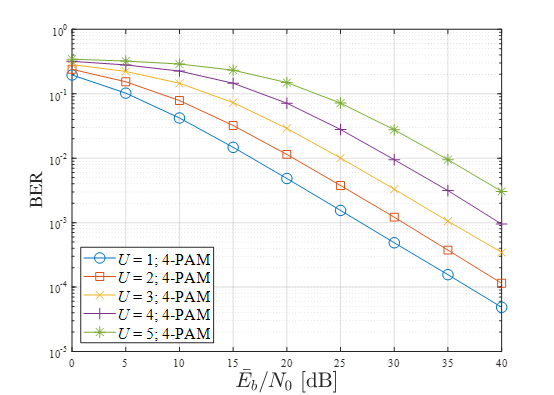
\includegraphics[width=15cm]{fig/gdma_4_PAM_implement.png}
 \caption{BER performances of uncoded GDMA 4-PAM system over block Rayleigh fading channels.}
 \label{fig:4_pam_implementation}
\end{figure}

\begin{figure}[t!]
 \centering
 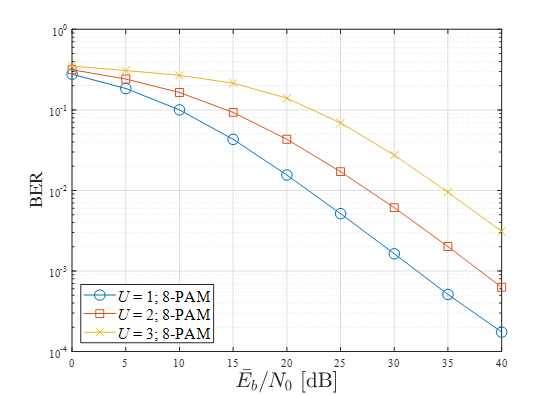
\includegraphics[width=15cm]{fig/gdma_8_PAM_implement.png}
 \caption{BER performances of uncoded GDMA 8-PAM system over block Rayleigh fading channels.}
 \label{fig:8_pam_implementation}
\end{figure}

Fig.\ref{fig:4_pam_implementation} and fig.\ref{fig:8_pam_implementation} are the BER performance respectively for uncoded GDMA 4-pam and 8-pam.


\begin{figure}[H]
 \centering
 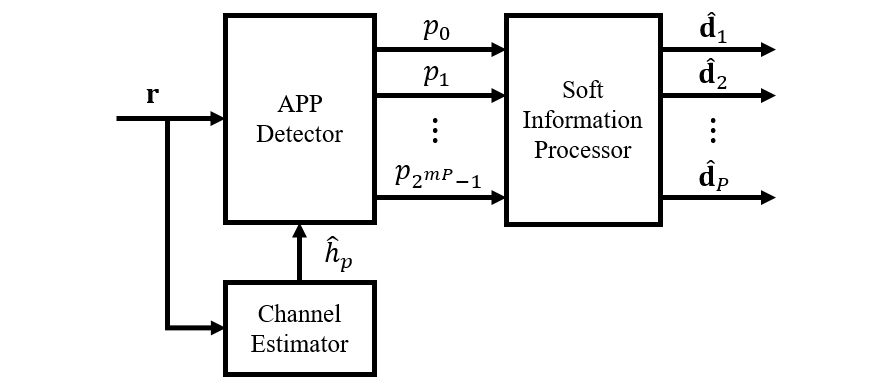
\includegraphics[width=15cm]{fig/gdma_rx.png}
 \caption{Multi-level receiver in GDMA system for recovering the messages of U users.}
 \label{fig:gdma_rx}
\end{figure}


The LLRs can be directly used for data detection or be further fed to the following soft information processor (SIP) when FEC coding is considered. The block diagram of the multiuser detector in GDMA system is shown in Fig.~\ref{fig:gdma_rx}. The SIP can be implemented by using several decoders (DECs) and one for each user independently as shown in Fig.~\ref{fig:gdma_scd}. A joint channel decoder can be an alternative to implement the SIP and extract the messages of all users simultaneously. The implementation of SIP will be discussed in Sec.~\ref{s:mldt_fec}. 
If the messages are transmitted without FEC coding, the decision rule with the APPs derived from multi-level detection is equivalent to finding the nearest neighbor of received symbol among all the levels. The corresponding decision region depends on the channel coefficients.

\begin{figure}[H]
 \centering
 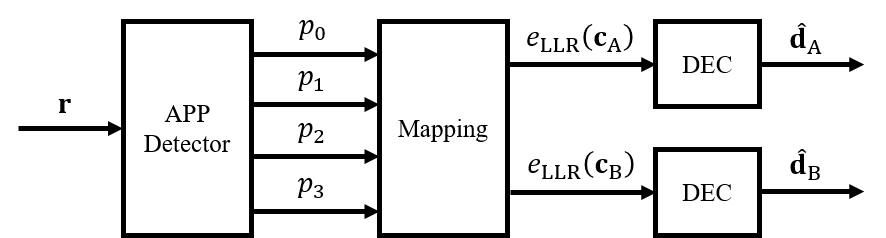
\includegraphics[width=15cm]{fig/gdma_scd.png}
 \caption{Separated channel decoding in the case of $m=1$ and $U=2$.}
 \label{fig:gdma_scd}
\end{figure}

%==================================================
\section{Joint channel decoding for the GDMA system}
\label{s:mldt_fec}

In this section, the implementation flow of the soft information processor (SIP) in the multiuser detector is discussed. We firstly review the joint channel decoding for the LDPC coded GDMA system and secondly discuss a novel joint channel decoding for the polar coded system.

%--------------------------------------------------

\subsection{Introduction of Joint Channel Decoding}

A straightforward method to construct the SIP in GDMA system is called separated channel decoding (SCD) as shown in fig.~\ref{fig:gdma_scd}. To recover the messages of $U$ users in GDMA-SCD system, the APPs of code bits are first attained and then be fed to the following decoders independently for each user. Note that there is no exchange of informations between collided users in GDMA-SCD scheme.

Another method of FEC-GDMA system is called Joint Channel Decoding (JCD) as shown in \ref{fig:gdma_jcd}, an alternative to implement the SIP in the case of $U=2$ and BPSK transmission. In the GDMA-JCD system, The APPs of codeword will pass the message to the JCD decoder before mapping LLRs. In the JCD, $L$ APP vectors will pass to JCD decoder, therefore, the APPs will be more reliable. However, the amount of messages passing is $L$ times of SCD, the operation complexity will be an exponentially increase.


\begin{figure}[t!]
 \centering
 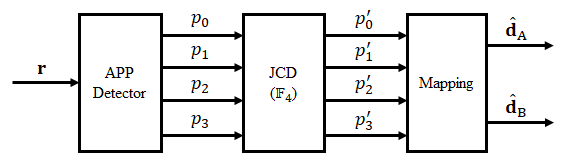
\includegraphics[width=15cm]{fig/gdma_jcd.png}
 \caption{Joint channel decoding in the case of $m=1$ and $U=2$.}
 \label{fig:gdma_jcd}
\end{figure}

\subsection{LDPC Coded GDMA system}

A generalized joint channel decoding and physical-layer network coding (G-JCNC) in \cite{gjcnc10}. The G-JCNC was proposed to combine the soft decoding of LDPC codes and the physical-layer network coding (PLNC), and here we take advantage of joint channel decoding (JCD) to extract the messages of $U$ users simultaneously. The APPs of each symbol $s(n)$, $p_l$ with $l \in \{0, 1, ..., 2^{mU}-1\}$, are sent to a non-binary decoder using generalized SPA (G-SPA), and the decoding is performed with respect to $\mathbb{F}_{2^{mU}}$. The procedure of G-SPA in the case of $U=2$ and BPSK transmission is described as follows.


\paragraph{Messages and Initialization}

An LDPC code can be represented as a bipartite graph, called Tanner graph, defined by the parity-check matrix with two kinds of nodes: check nodes and variable nodes. The G-SPA iteratively determines the APPs of the symbol $s(n)$ with $n \in \{1, 2, ..., N_c\}$ over the Tanner graph \cite{spa01}. The four possible levels in each $s(n)$ are shown in Table~\ref{table:mapping_m1_p2}. The message passed through the edges in the corresponding Tanner graph are represented by probability vector ${\bf p} = [ \ p_0 \ p_1 \ p_2 \ p_3 \ ]$ where $p_i$ is the probability that the value of variable $s(n)$ is $S[l]$ with $l \in \{0, 1, 2, 3\}$, and $ p_0+p_1+p_2+p_3=1$ holds. The initial message of variable node $s(n)$ given the received symbol $r(n)$ is $p_{l} = \text{Pr}\left\{s(n) = S[l]\middle|r\right\}$ with $l \in \{0, 1, 2, 3\}$ given in (\ref{equ:app}). 

The message updating rules at variable nodes and check nodes within the G-SPA are the same as that discussed in \cite{spa01}, and the update functions are defined as $\text{VAR}$ and $\text{CHK}$ for variable nodes and check nodes respectively. The discussion is restricted to nodes of degree three and the messages from the nodes with degree greater than three can be calculated by
\begin{align}
 \text{VAR}({\bf p}, {\bf q}, \cdots) & = {\textrm{VAR}}({\bf p}, {\textrm{VAR}}({\bf q}, {\textrm{VAR}}(\cdot, \cdot))) , \nonumber \\
 \text{CHK}({\bf p}, {\bf q}, \cdots) & = {\textrm{CHK}}({\bf p}, {\textrm{CHK}}({\bf q}, {\textrm{CHK}}(\cdot, \cdot))) ,
\end{align}
where ${\bf p}$ and ${\bf q}$ denote the corresponding input messages derived from variable nodes or check nodes. The functions of $\text{VAR}$ and $\text{CHK}$ at the nodes of degree three are illustrated in Fig.~\ref{fig:gspa_msg}, and the circles and squares represent the variable nodes and check nodes respectively. 

\begin{figure}[b!]
 \centering
 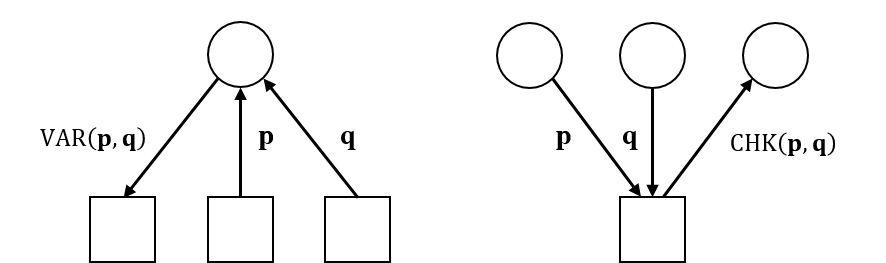
\includegraphics[width=15cm]{fig/gspa_msg.png}
 \caption{The message passing algorithm along the edges in factor graph.}
 \label{fig:gspa_msg}
\end{figure}

\paragraph{Output Message of Variable Nodes}

When the two input messages ${\bf p} = [ \ p_0 \ p_1 \ p_2 \ p_3 \ ]$ and ${\bf q} = [ \ q_0 \ q_1 \ q_2 \ q_3 \ ]$ arrive at the variable node $s(n)$, the probability that $s(n)=S[l]$ with $l \in \{0 ,1, 2, 3\}$ is given by
\begin{align}
 \text{Pr}\{s(n)=S[l]|{\bf p}, {\bf q}\} & = \frac{\text{Pr}\{{\bf p}, {\bf q}|s(n)=S[l]\}\text{Pr}\{s(n)=S[l]\}}{\text{Pr}\{{\bf p}, {\bf q}\}} \nonumber \\
 & = \frac{\text{Pr}\{s(n)=S[l]|{\bf p}\}\text{Pr}\{s(n)=S[l]|{\bf q}\}\text{Pr}\{{\bf p}\}\text{Pr}\{{\bf q}\}}{\text{Pr}\{{\bf p}, {\bf q}\}} \nonumber \\
 & = \beta p_l q_l ,
\end{align}
where
\begin{align}
 \beta = \frac{\text{Pr}\{{\bf p}\}\text{Pr}\{{\bf q}\}}{\text{Pr}\{{\bf p}, {\bf q}\}} = \frac{1}{p_0 q_0 + p_1 q_1 + p_2 q_2 + p_3 q_3} ,
\end{align}
is a normalization factor. Therefore, the output message of variable node $s(n)$ is
\begin{align}
 \text{VAR}({\bf p}, {\bf q}) = \beta [ \ p_0 q_0 \ p_1 q_1 \ p_2 q_2 \ p_3 q_3 \ ] .
\end{align}

\paragraph{Output Message of Check Nodes}

A specific parity-check equation is satisfied if the $\mathbb{F}_4$ sum of the connected quaternary symbols in the corresponding Tanner graph is equal to zero, i.e., $s(n) \oplus s(n_1) \oplus s(n_2) = 0$. Assuming that the two input messages derived from the variable nodes $s(n_1)$ and $s(n_2)$ are ${\bf p} = [ \ p_0 \ p_1 \ p_2 \ p_3 \ ]$ and ${\bf q} = [ \ q_0 \ q_1 \ q_2 \ q_3 \ ]$, respectively. The probability that the parity-check equation is satisfied under the the assumption that $s(n)=S[0]$ is
\begin{align}
 \text{Pr}\{s(n)=S[0]|{\bf p}, {\bf q}\} = & \quad \text{Pr}\{s(n_1)=S[0], s(n_2)=S[0]|{\bf p}, {\bf q}\} \nonumber \\
 & + \text{Pr}\{s(n_1)=S[1], s(n_2)=S[1]|{\bf p}, {\bf q}\} \nonumber \\
 & + \text{Pr}\{s(n_1)=S[2], s(n_2)=S[2]|{\bf p}, {\bf q}\} \nonumber \\
 & + \text{Pr}\{s(n_1)=S[3], s(n_2)=S[3]|{\bf p}, {\bf q}\} \nonumber \\
 = & \quad p_0 q_0 + p_1 q_1 + p_2 q_2 + p_3 q_3.
\end{align}
Similarly we can have
\begin{align}
 \text{Pr}\{s(n)=S[1]|{\bf p}, {\bf q}\} & = p_0 q_1 + p_1 q_0 + p_2 q_3 + p_3 q_2, \nonumber \\
 \text{Pr}\{s(n)=S[2]|{\bf p}, {\bf q}\} & = p_0 q_2 + p_2 q_0 + p_1 q_3 + p_3 q_1, \nonumber \\
 \text{Pr}\{s(n)=S[3]|{\bf p}, {\bf q}\} & = p_0 q_3 + p_3 q_0 + p_1 q_2 + p_2 q_1.
\end{align}
Finally, the message out of one check node equals
\begin{equation}
 \text{CHK}({\bf p},{\bf q})= \left[
 \begin{split}
  &p_0 q_0 + p_1 q_1 + p_2 q_2 + p_3 q_3 \\
  &p_0 q_1 + p_1 q_0 + p_2 q_3 + p_3 q_2 \\
  &p_0 q_2 + p_2 q_0 + p_1 q_3 + p_3 q_1 \\
  &p_0 q_3 + p_3 q_0 + p_1 q_2 + p_2 q_1
 \end{split}
 \right]^T.
\end{equation}

\paragraph{Finalization and Symbol-to-Bit Mapping}

The decoding algorithm is stopped if all parity-check equations are fulfilled or the maximum number of iterations is reached. Otherwise, the process proceed with further iteration until one of the conditions is satisfied. At the end of the decoding algorithm, the G-SPA generates the APP vector ${\bf p} = [ \ p_0 \ p_1 \ p_2 \ p_3 \ ]$  with $p_i = \text{Pr}\left\{s(n) = S[l]\middle|r\right\}$ for each symbol $s(n)$ with $n \in \{1, 2, ..., N_c\}$ and the symbol-to-bit mapping is done by (\ref{equ:bit_mapping}). The combination of multi-level detection and G-SPA is referred to as GDMA-JCD scheme in this thesis. The G-SPA with higher-order modulation scheme was investigated in \cite{gjcncqpsk10}. 

\paragraph{Simulation Results} 

The BLER performances of GDMA-JCD and GDMA-SCD systems using a (1008, 504) rate-1/2 binary (3,6)-regular LDPC code with BPSK transmissions over quasi-static Rayleigh flat-fading channels are provided in Fig.~\ref{fig:bler_ldpc}. The maximum number of decoding iterations is set to 50 for both SPA and G-SPA. In the transmissions over block flat-fading channels, the GDMA-JCD scheme outperforms the GDMA-SCD scheme in low-SNR region and the performances of two schemes converge to each other in high-SNR region. We further consider an OFDM-GDMA system that has $16$ sub-carrier and $63$ bits for each sub-carrier symbol. The BLER performance of GDMA-OFDM-JCD and GDMA-OFDM-SCD using same parameters as above and are provided in Fig.~ \ref{fig:bler_ofdm_ldpc}. We found that JCD can effectively use different user information, even when increasing the number of users, performance has almost no loss.


\begin{figure}[t!]
 \centering
 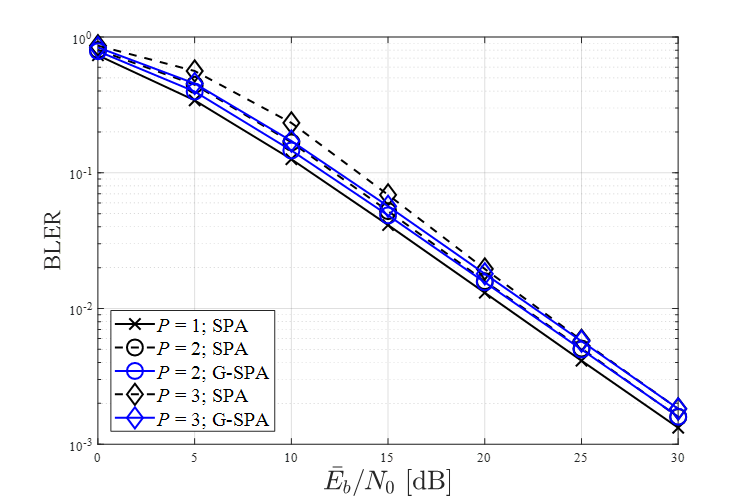
\includegraphics[width=14cm]{fig/bler_ldpc.png}
 \caption{BLER performances of (1008, 504) LDPC-coded GDMA systems over quasi-static Rayleigh flat-fading channels.}
 \label{fig:bler_ldpc}
\end{figure}

\begin{figure}[b!]
 \centering
 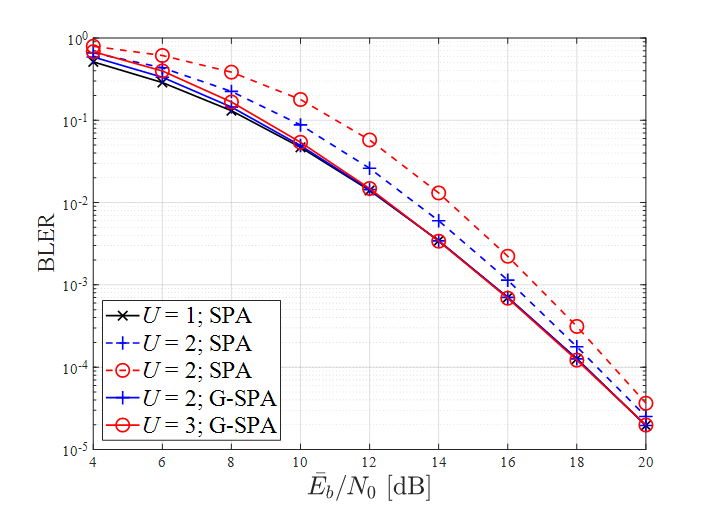
\includegraphics[width=14cm]{fig/bler_gdma_ofdm_ldpc.png}
 \caption{BLER performances of (1008, 504) LDPC-coded GDMA OFDM systems over quasi-static Rayleigh flat-fading channels with 16-subcarrier.}
 \label{fig:bler_ofdm_ldpc}
\end{figure}

\subsection{Polar Coded GDMA system}

	Polar code \cite{polar09} invented by Erdal Arikan in 2006 can achieve symmetric capacity on binary-input discrete memoryless channels. In 5G standardization, polar code has been adopted as a channel coding scheme for 3GPP new radio(NR) access technology. By exploiting channel polarization, one can construct excellent polar codes, and employ low-complexity successive cancellation(SC), successive cancellation list (SCL)\cite{scl15}, and sum-product Algorithm(SPA)\cite{arikan2010polar} for polar codes. In the thesis\cite{yt19}, the polar coded GDMA system was implemented by separated channel decoding (SCD) with SCL decoder. Since the hard decoding structure in SCL decoder, it can not pass APP vectors directly. We need soft value  to map the codeword LLR $e_{LLR(n,u)}$ with $n\in\{1,2,…,N_c \};u\in\{1,…,U\}$ for each user. In this section, we firstly introduce a general sum-product algorithm (G-SPA) decoder and secondly a joint successive cancellation list (J-SCL) decoder for polar coded JCD-GDMA system.  
	
\paragraph{Graph representation}

	The graph representation Fig.\ref{fig:graph_presentaion} for the transformation was noticed by Forney who suggested a SPA decoder for RM codes using factor graph representation. Since Polar code is the family of RM code, \cite{arikan2010polar} use the graph of polar code structure to do SPA decoding. There are four nodes in a base computation block (BCB). Instead of passing LLR value, the JCD passes the probability vector of each level in the factor graph. We define the vectors passing to the right as $\bf{R_{i,j}}$ and the vectors passing to the left as $\bf{L_{i,j}}$ where $1 \leq i \leq n+1, 1 \leq j \leq N, \ N:\text{codeword length}, \ n:\text{factor graph layer}$. The nodes of factor graph are labelled with pairs of integers $(i,j)$. From the decoder's perspective, the leftmost nodes, $(n+1,j)$ are associate with the source vector ${\bf u}=[u_0  \ u_1 \ u_2 \ \cdots  \ u_L]$ where $u_{j}$ is the message information of each user, while the rightmost nodes ($1,j)$ are associated with channel input vectors ${\bf p}=[p_0  \ p_1 \ p_2 \ \cdots  \ p_L]$ where $p_l$ is the probability that are observed through a noisy channel. Instead of min sum operations, we define the BCB upper branch calculations as $f$-function and lower branch calculations as $g$-function such as Fig.\ref{fig:BCB function}. For clarity, we predigest $g$-function a vector product calculation, $f$-function a vector parity check calculation. The function definition in the case of $U=2$ and BPSK transmission is described as follows. Fig.\ref{fig:graph_presentaion} is the graph representation example for $N=8, n=3$, where BCB in fig.\ref{fig:BCB function} is the unit of graph. $g$-function and $f$-function are the operations same as generalized joint channel decoding and physical-layer network coding (G-JCNC) in \cite{gjcnc10}. 
	

\begin{figure}[t!]
 \centering
 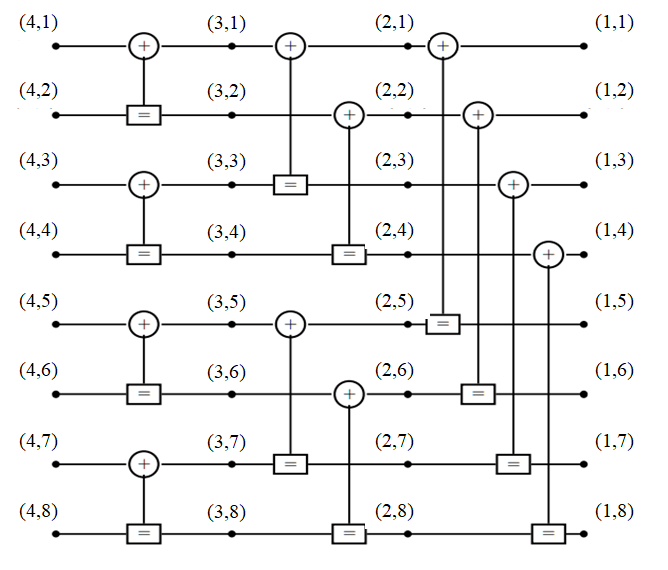
\includegraphics[width=12cm]{fig/graph_presentation.png}
 \caption{The graph factor for polor code, $N=8, n=3$.}
 \label{fig:graph_presentaion}
\end{figure}

\begin{figure}
 \centering
 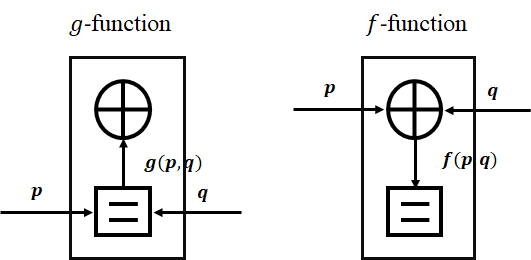
\includegraphics[width=10cm]{fig/BCB_function.png}
 \caption{The message passing function in factor graph.}
 \label{fig:BCB function}
\end{figure}



\paragraph{$f$-function}

When the two input messages vectors ${\bf p} = [ \ p_0 \ p_1 \ p_2 \ p_3 \ ]$ and ${\bf q} = [ \ q_0 \ q_1 \ q_2 \ q_3 \ ]$ arrive at the BCB upper branches $s(n)$, the probability that $s(n)=S[l]$ with $l \in \{0 ,1, 2, 3\}$ is given by
\begin{align}
 \text{Pr}\{s(n)=S[l]|{\bf p}, {\bf q}\} & = \frac{\text{Pr}\{{\bf p}, {\bf q}|s(n)=S[l]\}\text{Pr}\{s(n)=S[l]\}}{\text{Pr}\{{\bf p}, {\bf q}\}} \nonumber \\
 & = \frac{\text{Pr}\{s(n)=S[l]|{\bf p}\}\text{Pr}\{s(n)=S[l]|{\bf q}\}\text{Pr}\{{\bf p}\}\text{Pr}\{{\bf q}\}}{\text{Pr}\{{\bf p}, {\bf q}\}} \nonumber \\
 & = \beta p_l q_l ,
\end{align}
where
\begin{align}
 \beta = \frac{\text{Pr}\{{\bf p}\}\text{Pr}\{{\bf q}\}}{\text{Pr}\{{\bf p}, {\bf q}\}} = \frac{1}{p_0 q_0 + p_1 q_1 + p_2 q_2 + p_3 q_3} ,
\end{align}
is a normalization factor. Therefore, the output message is
\begin{align}
 f({\bf p}, {\bf q}) = \beta [ \ p_0 q_0 \ p_1 q_1 \ p_2 q_2 \ p_3 q_3 \ ] .
\end{align}

\paragraph{$g$-function}
	
A specific parity-check equation is satisfied if the $\mathbb{F}_4$ sum of the connected quaternary symbols in the corresponding Tanner graph is equal to zero, i.e., $s(n) \oplus s(n_1) \oplus s(n_2) = 0$. Assuming that the two input messages derived from the variable nodes $s(n_1)$ and $s(n_2)$ are ${\bf p} = [ \ p_0 \ p_1 \ p_2 \ p_3 \ ]$ and ${\bf q} = [ \ q_0 \ q_1 \ q_2 \ q_3 \ ]$, respectively. The probability that the parity-check equation is satisfied under the the assumption that $s(n)=S[0]$ is
\begin{align}
 \text{Pr}\{s(n)=S[0]|{\bf p}, {\bf q}\} = & \quad \text{Pr}\{s(n_1)=S[0], s(n_2)=S[0]|{\bf p}, {\bf q}\} \nonumber \\
 & + \text{Pr}\{s(n_1)=S[1], s(n_2)=S[1]|{\bf p}, {\bf q}\} \nonumber \\
 & + \text{Pr}\{s(n_1)=S[2], s(n_2)=S[2]|{\bf p}, {\bf q}\} \nonumber \\
 & + \text{Pr}\{s(n_1)=S[3], s(n_2)=S[3]|{\bf p}, {\bf q}\} \nonumber \\
 = & \quad p_0 q_0 + p_1 q_1 + p_2 q_2 + p_3 q_3.
\end{align}
Similarly we can have
\begin{align}
 \text{Pr}\{s(n)=S[1]|{\bf p}, {\bf q}\} & = p_0 q_1 + p_1 q_0 + p_2 q_3 + p_3 q_2, \nonumber \\
 \text{Pr}\{s(n)=S[2]|{\bf p}, {\bf q}\} & = p_0 q_2 + p_2 q_0 + p_1 q_3 + p_3 q_1, \nonumber \\
 \text{Pr}\{s(n)=S[3]|{\bf p}, {\bf q}\} & = p_0 q_3 + p_3 q_0 + p_1 q_2 + p_2 q_1.
\end{align}
Finally, the message out of one check node equals
\begin{equation}
 \text{CHK}({\bf p},{\bf q})= \left[
 \begin{split}
  &p_0 q_0 + p_1 q_1 + p_2 q_2 + p_3 q_3 \\
  &p_0 q_1 + p_1 q_0 + p_2 q_3 + p_3 q_2 \\
  &p_0 q_2 + p_2 q_0 + p_1 q_3 + p_3 q_1 \\
  &p_0 q_3 + p_3 q_0 + p_1 q_2 + p_2 q_1
 \end{split}
 \right]^T.
\end{equation}


\subsubsection{General Sum Product Algorithm decoder}


	In addition to SCL decoder, SPA decoder can also be used to decode polar code. We can replace this SPA decoder with the G-SPA decoder, e.g., passing APP vector in factor graph by $f$ and $g$ functions. It can be easily converted separated channel decoding into joint channel decoding GDMA (JCD-GDMA) system.  
	
\paragraph{Initialization}
	
	In G-SPA, we changed the LLR representation to vector representation, and before message passing, we need to set the initial vectors. For simplicity, we set the initial vectors on the most left as the initial APPs of the received superimposed signal. The rightest vectors are determined according to the frozen bits of the polar code, and the other vectors are the message.

The rightmost nodes $(1, j)$ are associated with channel input vectors that are observed through a noisy channel, $1 \leq i \leq n+1, 1 \leq j \leq N$ where $N$ is the codeword length. 
\begin{align}
L_{1,j} = [p_0 \quad p_1 \cdots p_L]. \quad p_l = \text{Pr}\{s=S[l]|r\}
\end{align}

The leftmost nodes, $(n+1, j)$, are associated with the source data that are to be estimated. If $u_j$ is a frozen bit, we can determine that the leftmost $R_{n+1.j}$ is equal to the superimposed signal $S[0]$, so it can be represented as


\begin{equation}
R_{n+1.j}
\nonumber \\ = 
\left\{
             \begin{array}{lr}
             { [1 \quad 0 \quad \cdots \quad 0] }, \ \text{if  is a frozen coordinate} &  \\
           { [ \frac{1}{L} \quad \frac{1}{L} \quad \cdots \quad \frac{1}{L} ] },  \ \text{if  is an infrozen coordinate}& \\ 
             \end{array}
\right.
\end{equation}

All the other nodes $R_{i.j}$ and $L_{i.j}$ are setted equal to $[\frac{1}{L} \quad \frac{1}{L} \quad \cdots \quad \frac{1}{L}]$ 


\begin{figure}[t!]
 \centering
 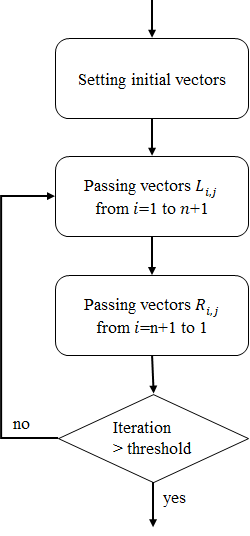
\includegraphics[width=5cm]{fig/polar_gspa_flowchart.png}
 \caption{The flow chart of polar code G-SPA decoder.}
 \label{fig:polar_gspa_flowchat}
\end{figure}

\paragraph{Message passing}

	After setting initial vectors of the factor graph, the massage passing procedure is as fig.\ref{fig:polar_gspa_flowchat}. Unlike the SCL decoder, all operations in the SPA decoder are parallel. The operations will start from the rightmost nodes, then pass the message vectors to the left in sequence. Until updating to the leftmost node, and then act to the right nodes. When it updates to the rightmost nodes again, it finishes an iteration. The BCB calculation is described as

\begin{align}
L_{i+1,\ j} = f \{ L_{i, \ j + N_i}, \ g\{L_{i, \ j}, R_{i, \ j} \} \} \nonumber \\
L_{i+1, \ j+N_i} = g \{ L_{i, \ j + N_i}, \ f\{L_{i, \ j}, \  R_{i+1, \ j} \} \} \nonumber \\
R_{i, \ j} = f \{ R_{i+1, \ j}, \ g\{L_{i, \ j+N_i}, \ R_{i+1, \ j+N_i} \} \} \nonumber \\
R_{i, \ j+N_i} = f \{ R_{i+1, \ j+N_i}, \ g\{L_{i,j}, \ R_{i+1, \ j} \} \} 
\end{align}
, where $N_i=2^{n-i}$ is the connection between each nodes.


\paragraph{Simulation result}

 We now compare the decoders using SPA and using G-SPA. The BLER performances of GDMA-JCD and GDMA-SCD systems using a (256, 128) rate-1/2 Polar code with BPSK transmissions over quasi-static Rayleigh flat-fading channels are provided in Fig.~\ref{fig:bler_polar_spa}. The maximum number of decoding iterations is set to 50 for both SPA and G-SPA. In the transmissions over block flat-fading channels, the GDMA-JCD scheme outperforms the GDMA-SCD scheme in low-SNR region, and the performances of two schemes converge to each other in high-SNR region. Since the block fading systems are lack of channel diversity, e.g., the probability of deep fading is very high, and the coding gain is not obvious. Hence, we further consider an OFDM-GDMA system that can obtain channel diversity from each sub-carrier using a (1024, 512) rate-1/2 Polar code that has $16$ sub-carrier and $64$ bits for each sub-carrier symbol. The BLER performance of GDMA-OFDM-JCD and GDMA-OFDM-SCD using the same parameters as above and are provided in Fig.\ref{fig:bler_ofdm_polar_spa}. We found that JCD can effectively use different user information, even when increasing the number of users, performance has almost no loss.

\begin{figure}[H]
 \centering
 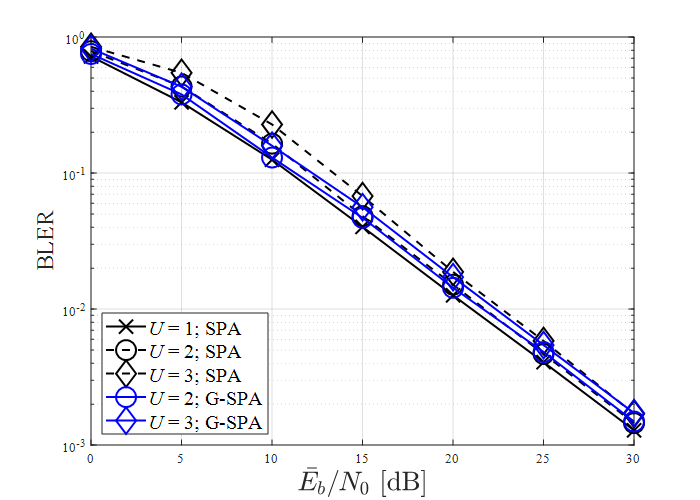
\includegraphics[width=14cm]{fig/bler_polar_spa.png}
 \caption{BLER performances of (256, 128) Polar-coded GDMA systems over quasi-static Rayleigh flat-fading channels.}
 \label{fig:bler_polar_spa}
\end{figure}

\begin{figure}[H]
 \centering
 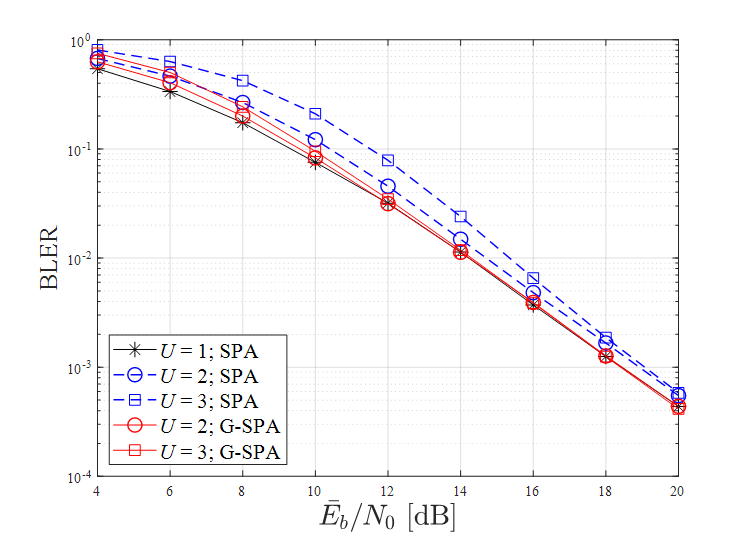
\includegraphics[width=14cm]{fig/bler_gdma_ofdm_polar_spa.png}
 \caption{BLER performances of (1024, 512) Polar-coded GDMA OFDM systems over quasi-static Rayleigh flat-fading channels with 16-subcarrier.}
 \label{fig:bler_ofdm_polar_spa}
\end{figure}

\subsubsection{Joint Successive Cancellation List decoder}

 There are some well-known decoders such as SPA\cite{arikan2010polar}, SCL \cite{scl15}, and SCAN for polar codes. These decoders have their advantages, such as SPA decoder, which is very simple in hardware implementation, and SCL with CRC is able to achieve the best performance in AWGN channel. Compared with the parallel operation of the SPA decoder, the SCL decoder's operation is in a specific order. For implementing a joint successive cancellation list (J-SCL)decoder, we still use $\bf{L_{i,j}}$  $\bf{R_{i,j}}$  to represent the message vectors and $f$-function $g$-function as the operation calculator where $g$-function a vector product calculation, $f$-function a vector parity check calculation. 

Before message passing, we need to set the initial vectors. For simplicity, we set the initial vectors on the rightmost nodes as the  APPs of the superimposed signals. Compared to the G-SPA decoder, the J-SCL decoder does not initialize the other node values.

The rightmost nodes (n+1, j) are associated with channel input vectors $\bf{p}$ that are observed through a noisy channel. 
\begin{align}
{\bf{L_{i,j}}} = [p_0 \quad p_1 \cdots p_L]. \quad {\bf{p_l}} = \text{Pr}\{s=S[l]|r\}
\end{align}

\paragraph{Update for odd branch}

Fig.\ref{fig:jscl_uplayer} and equ. \ref{equ:scl_odd} show a basic computation unit for odd channels. The vectors passing to odd channels can be computed via recursion until leftmost nodes. If passing to the leftmost unfrozen nodes, it will map to the LLR value $e_{\text{LLR}}[c_{j,u}]$ according to mapping rules in chapter-\ref{c:gdma} and obtain a message bit $\hat{u}_{j,u}$ that is the hard decoding value for the $j$-th codeword and $u$-user.

\begin{align}
{\bf{L_{i+1,j}}} = f({\bf L_{i,j}, \ L_{i,j+N_t}})
\label{equ:scl_odd}
\end{align}

\begin{figure}[H]
 \centering
 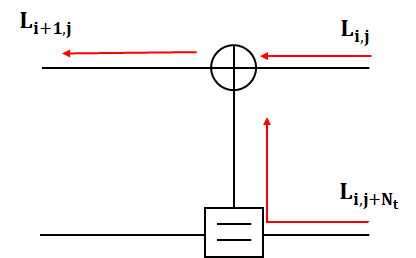
\includegraphics[width=8cm]{fig/jscl_uplayer.png}
 \caption{The factor graph of J-SCL upper layer (even branch) message passing.}
 \label{fig:jscl_uplayer}
\end{figure}


\paragraph{Update for even branch}
Fig.\ref{fig:jscl_lowlayer} and equ.\ref{equ:scl_even} show a basic computation unit for even channels. The vectors passing for even channels can also be computed via recursion. Instead of passing soft right propagating vectors $R_{i+1,j}$ in the G-SPA decoder, the vectors $\bf R_{i+1,j}$ are hard feedback vectors according to message bits $\hat{u}_{j,u}, u \in \{ 1, \cdots, U\}$.

\begin{align}
{\bf{L_{i+1,j+N_i}}} = g( {\bf{L_{i+1,j+N_i}}}, \ f ({\bf{ L_{i+1,j}}} , {\bf{R_{i+1,j}}}) )
\label{equ:scl_even}
\end{align}

Assume that $U=2$ and BPSK transmission, the feedback vectors $\bf R_{i+1,j}$ are described as : 
\begin{align}
\text{if} \  \hat{u}_{j,1}= 0 \ \text{and} \ \hat{u}_{j,2}= 0, {\bf R_{n+1,j}} = {[1 \ 0 \ 0 \ 0]} \nonumber \\
\text{if} \  \hat{u}_{j,1}= 0 \ \text{and} \ \hat{u}_{j,2}= 1, {\bf R_{n+1,j}} = {[0 \ 1 \ 0 \ 0]} \nonumber \\
\text{if} \  \hat{u}_{j,1}= 1 \ \text{and} \ \hat{u}_{j,2}= 0, {\bf R_{n+1,j}} = {[0 \ 0 \ 1 \ 0]} \nonumber \\
\text{if} \  \hat{u}_{j,1}= 1 \ \text{and} \ \hat{u}_{j,2}= 1, {\bf R_{n+1,j}} = {[0 \ 0 \ 0 \ 1]} \nonumber 
\end{align}



\begin{figure}[H]
 \centering
 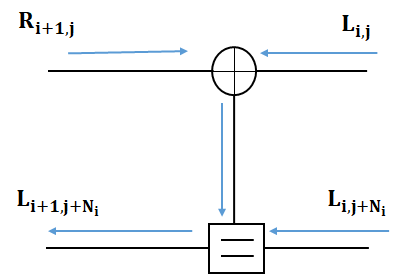
\includegraphics[width=8cm]{fig/jscl_lowlayer.png}
 \caption{The factor graph of J-SCL lower layer (odd branch) message passing.}
 \label{fig:jscl_lowlayer}
\end{figure}

Once obtain $\bf{R_{n+1,j}}$ from the leftmost nodes, we can also derive right propagating vectors $\bf{R_{i,j}}$ via recursion as

\begin{align}
{\bf{R_{i,j}}} = f ( \bf R_{i+1,j} , R_{i+1,j+N_i}) ) \nonumber  \\
\bf{R_{i,j+N_i}} = R_{i+1,j+N_i}  \nonumber
\end{align}
 

\paragraph{Metric path}

After obtain the leftmost probability vectors, we convert probability vectors to the LLR values $e_{\text{LLR}} [c_{j,u} ]$  where $u \in \{1,2,…,U\}  j \in \{1,2,…,N\}$ of each user, which can be obtained by the above formula. Besides, we must record the PM value of this period where PM value is used in list decoding to record the LLR value of each metric path. SCL decoder will only have two forks per path, which are LLR values equal to 0 or 1  respectively. Different from SCL decoder, the forks of each J-SCL path is $L = 2^{mU}$ since the path metric $\text{PM}_l^i$ must contain each user hard decoding information, where $L$ is the number of superimposed signals, we can express the expression as follows:

For the $l$-th path and the $i$-th level, $i=1,2,\cdots,N$, the PM value is given by


\begin{align}
\text{PM}_l^i \triangleq \sum_{j=1}^{i} \sum_{u=1}^{U} \text{ln} \{ 1+\text{exp}[-(1-2 \hat{u}_{j,u} ) e_{\text{LLR}})] \}
\end{align}
where $\hat{u}_{j,u}$ are the hard decoding value for the $j$-th codeword and $u$-th user according to $e_\text{LLR} [c_{j,u} ]$. 

\paragraph{Simulation result}
The BLER performances of GDMA-JCD and GDMA-SCD systems using a (256, 128) rate-1/2 Polar code with CRC-16 BPSK transmissions over quasi-static Rayleigh flat-fading channels are provided in Fig.~\ref{fig:bler_polar_scl}. The maximum number of decoding iterations is set to 50 for both SPA and G-SPA. In the transmissions over block flat-fading channels, the GDMA-JCD scheme outperforms the GDMA-SCD scheme in low-SNR region, and the performances of two schemes converge to each other in high-SNR area. We further consider an OFDM-GDMA system using a (1024, 512) rate-1/2 Polar code with CRC-16 that has $16$ sub-carrier and $64$ bits for each sub-carrier symbol. The BLER performance of GDMA-OFDM-JCD and GDMA-OFDM-SCD using the same parameters as above and are provided in Fig.~ \ref{fig:bler_ofdm_polar_scl}. We found that JCD can effectively use different user information, even when increasing the number of users, performance has almost no loss.

\begin{figure}[b!]
 \centering
 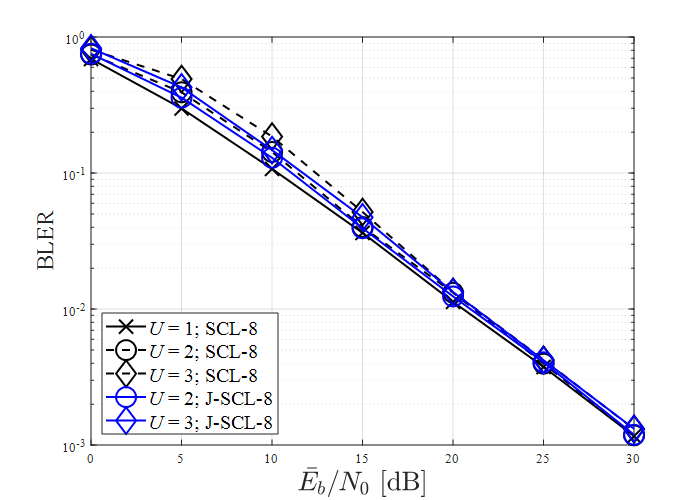
\includegraphics[width=14cm]{fig/bler_polar_scl.png}
 \caption{BLER performances of (256, 128) Polar-coded GDMA systems over quasi-static Rayleigh flat-fading channels.}
 \label{fig:bler_polar_scl}
\end{figure}


\begin{figure}[t!]
 \centering
 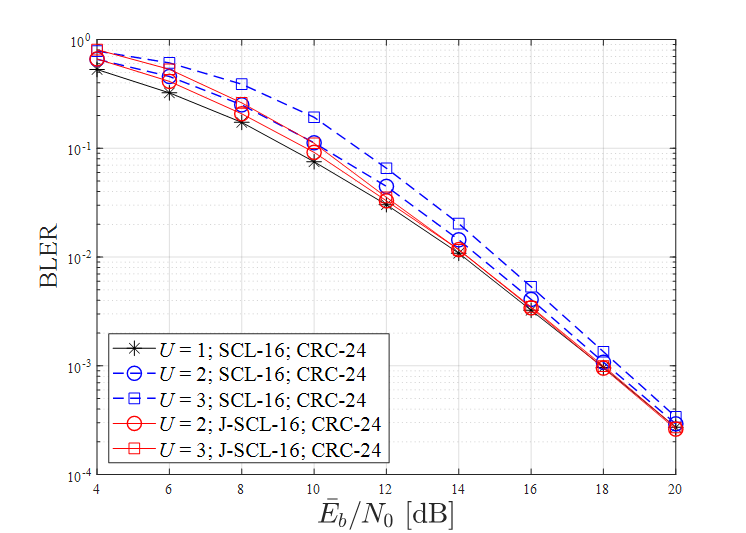
\includegraphics[width=14cm]{fig/bler_gdma_ofdm_polar_scl.png}
 \caption{BLER performances of (1024, 512) Polar-coded GDMA OFDM systems over quasi-static Rayleigh flat-fading channels with 16-subcarrier.}
 \label{fig:bler_ofdm_polar_scl}
\end{figure}

\begin{figure}[b!]
 \centering
 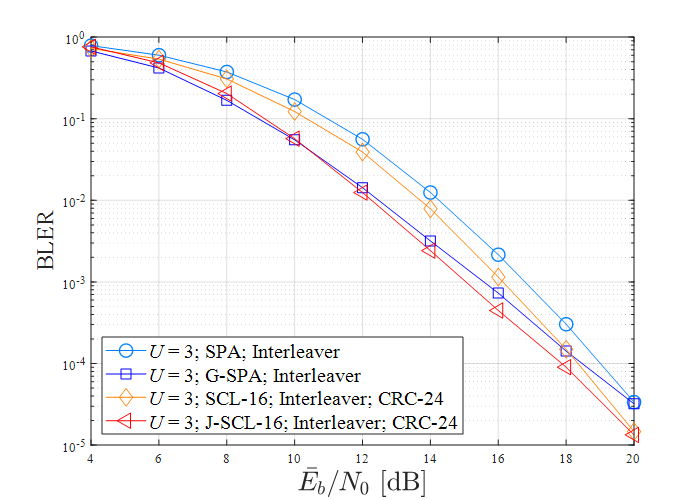
\includegraphics[width=14cm]{fig/bler_gspa_jscl_u3.png}
 \caption{BLER performances of Polar-coded GDMA OFDM systems over quasi-static Rayleigh flat-fading channels with 16-subcarrier and interleaver.}
 \label{fig:bler_ofdm_polar_scl_gspa}
\end{figure}


Since the polar construction is based on the same SNR of received signals, the received signals from OFDM system are distinct according to different energy of each sub-carrier channel gains. Hence, it can use interleaver to force the received signals into similar SNR, and the details were discussed in the paper \cite{lee2019curve}. In fig.\ref{fig:bler_ofdm_polar_scl_gspa}, we compare the performance of G-SPA and J-SCL decoder for polar code and assume code length of 1024, 16 sub-carrier OFDM system, $U=3$. Besides, add the interleaver to make the received massage to avoid sub-block deep fading. Then, add CRC check to SCL and J-SCL for better performance, where CRC length 24 is same as paper \cite{niu2012crc}. We can find that the JCD decoder's performance is better than SCD decoders from 4 dB to 18 dB, and different type decoders will converge in different performance in high SNR. 



\chapter{Cluster-Based Channel Estimation}
\label{c:cluster_ce}

\begin{figure}[b!]
 \centering
 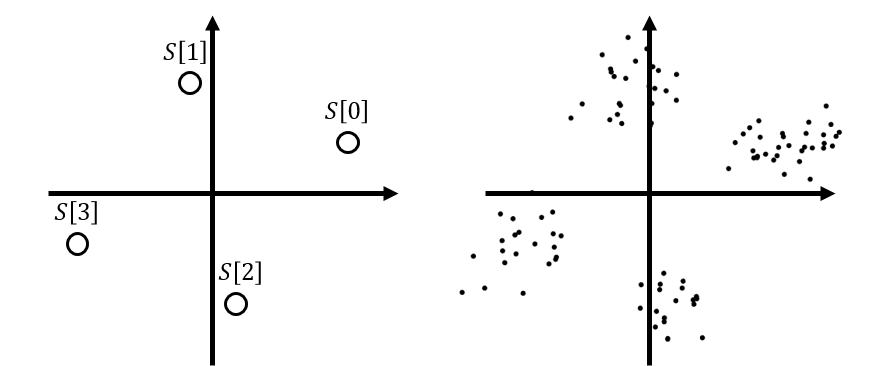
\includegraphics[width=15cm]{fig/rx_sig_m1_p2.bmp}
 \caption{Superimposed levels and the corresponding received signals in the case of $m=1$ and $U=2$.}
 \label{fig:rx_sig_m1_p2}
\end{figure}

In the thesis \cite{yt19}, the cluster-based channel estimation technique was proposed for efficient transmission. It used different clustering algorithms to analyze the mean square error (MSE) performance. However, it still couldn't achieve to  Cramer-Rao lower bound (CRLB) when $U$ was higher than two, and the proposed methods\cite{yt19} for deriving channel coefficients was a particular case that was only suitable for $U=2$ or $U=3$.  Hence, we proposed a general algorithm for clustering received signals and deriving the channel coefficient for any user and modulation.

\paragraph{Introduction for Cluster-based Channel Estimation}

When multiple users transmit through independent fading channels, the signals can be further separated by using different channel coefficients without requiring user-specific resources. The requirement for applying multi-level detection in the GDMA system is to accurately recover the channel coefficients at the receiver to construct all possible superimposed signal levels. Due to the presence of channel noise, the received signal in the block where the channel remains unchanged has a two-dimensional Gaussian distribution with mean $S[l]$ where $l \in \{0 \ ,1 \ , \cdots \ , 2^{mU} \}$ according to the messages of $U$ users. If we can classify the received symbols into a $2 ^ {mU} $ group in some way, where the symbols corresponding to the same level are grouped, the estimated value of the level can be obtained by the average value of the symbols in each group. In this section, we assume that he fading coefficients are constant across a block of $N_t$ consecutive symbols.  An example of the receive signals with $N_t$= 100 in the case of $m=1$ and $U=2$ is shown in Fig.\ref{fig:rx_sig_m1_p2}. Therefore, we use clustering algorithm to classify the received signals and blindly estimate the channel coefficients of $U$ users. Clustering is an unsupervised learning technique, which involves grouping training samples from different groups with different characteristics. Note that the clustering technique in the proposed scheme takes the signal with message as the input training sample, and since the estimation does not require additional pilot signals, it can achieve high frequency spectral efficiency and inevitable ambiguity in estimation.

%==================================================

\section{Review of Clustering Algorithm}

 Clustering is an unsupervised learning technique and the task of grouping a set of objects that called a cluster. In this section, we review the clustering algorithm survey from the thesis \cite{yt19}.

\subsection{K-Means Algorithm}
\label{s:clustering}

One of the most popular clustering techniques is the k-mean algorithm\cite {lloyd82}, which aims to minimize the sum of the square distance between each sample and its closest centroid. In the k-means problem, it is desirable to choose a set of centroids $S$ such that the following function can be minimized.

\begin{equation}
 \phi = \sum_{x \in X} \underset{s \in S}{\text{min}} \parallel x-s \parallel^2,
\end{equation}
where $X$ is the set of training vectors, and $\phi$ is the corresponding distortion. Therefore, K-means algorithm classifies samples by iteratively pairing each sample with the closest centroid, and then updating the centroid from the newly derived group.

For channel estimation in the GDMA system, all the levels should be distinguished. The number of groups to be classified is $2^{mU}$ in the clustering. The steps of the k-means algorithm are organized as follows.
\begin{enumerate}[leftmargin=\leftmargin+\widthof{Prefix}]
\item[Step 1)] Randomly pick the initial centroids from the symbols in the received sequence.
\item[Step 2)] Classify the received symbols into $2^{mU}$ groups by applying the nearest-neighbor rule with respect to the current centroids.
\item[Step 3)] Recompute the centroids by averaging the symbols in each group.
\item[Step 4)] Return to Step 2 until the centroids no longer change.
\end{enumerate}
The required number of iterations for clustering algorithms cannot be predicted ahead of time. In addition, the random seeding in the initial step of k-means may yield different grouping results in different runs of the algorithm.

In the k-means algorithm, the most crucial task is selecting acceptable initial centroids in the correct solution's neighborhood since it can only find a local minimum. Several clustering algorithms was proposed to select acceptable initial centroids such as LBG algorithm, k-mean++ algorithm, modified k-means++ algorithm.

%--------------------------------------------------

\subsection{The LBG Algorithm}

The Linde–Buzo–Gray (LBG) algorithm \cite{lbg80}, sometimes referred to as generalized Lloyd algorithm (GLA), is a technique to design vector quantizer and a so-called "splitting" method is employed to select the initial centroids for the following k-means clustering. The steps of LBG algorithm are organized as follows.
\begin{enumerate}[leftmargin=\leftmargin+\widthof{Prefix}]
\item[Step 1)] Split the origin into two close points $\epsilon$ and $-\epsilon$ and hence the set of initial centroids $S=\{\epsilon,-\epsilon\}$ with size $M=2$ is obtained.
\item[Step 2)] Classify the received symbols into $M$ groups, based on the current centroids $S$, by applying the nearest-neighbor rule and compute the centroid $\rho_i$ of each group with $i \in \{1, 2, ..., M\}$.
\item[Step 3)] Split $\rho_i$ into two close points $q_{2i-1}=\rho_i+\epsilon$ and $q_{2i}=\rho_i-\epsilon$ with $i \in \{1, 2, ..., M\}$ and the set of new centroids $S=\{q_i| i=1, 2, ...,2M\}$ is obtained.
\item[Step 4)] Replace $M$ by $2M$ and return to Step 2 until $M=2^{mU}$.
\item[Step 5)] Proceed with the standard k-means clustering.
\end{enumerate}

\begin{figure}[t!]
 \centering
 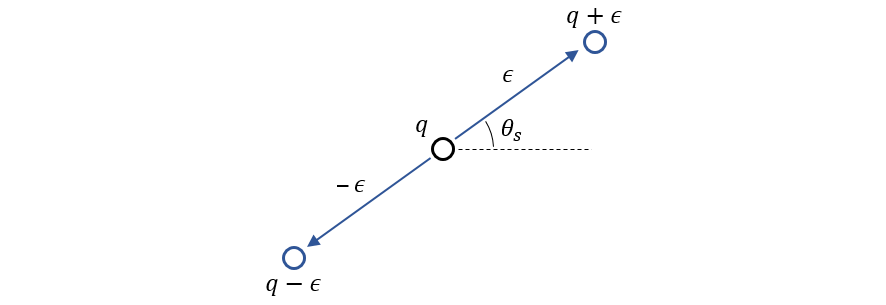
\includegraphics[width=15cm]{fig/lbg_splitting.png}
 \caption{Splitting from $q$ to get $q+\epsilon$ and $q-\epsilon$ with a perturbation vector $\epsilon$.}
 \label{fig:lbg_splitting}
\end{figure}

%--------------------------------------------------

\subsection{K-Means++ Algorithm}

The K-means + + algorithm is proposed in the \ {kmpp07} to select the initial centroid for the following K-means clustering, which can be regarded as a generalization of the standard k-means algorithm. The concept of K-means + + algorithm is to select the initial centroid as randomly as possible. Note that randomness is preserved in initialization, so K-means + + may not rely on the accuracy of training samples as LBG does. Let $D(r)$denote the distance from the received symbol $r$ to the closest centroid we have selected.

The steps of k-means++ algorithm are organized as follows.
\begin{enumerate}[leftmargin=\leftmargin+\widthof{Prefix}]
\item[Step 1)] Pick the first centroid $q_1$ uniformly at random from the symbols in received sequence and set $i=1$.
\item[Step 2)] Pick the next centroid $q_{i+1}$ from the remaining symbols with probability proportional to $D^2(r)$ and replace $i$ by $i+1$.
\item[Step 3)] Return to Step 2 until $i=2^{mU}$.
\item[Step 4)] Proceed with the standard k-means clustering.
\end{enumerate}


\subsection{Modified K-Means++ Algorithm}

The modified k-means++ algorithm was proposed in \cite{hsu2020uplink} to choose the initial centroids for the following k-means clustering, which can also be seen as a generalization of standard k-means algorithm. Compared to the k-means++ algorithm, it restricts the search space to a set $\Omega$ when selecting the next centroid $q_{i+1}$. This restriction might decrease the probability of selecting unsuitable initial centroids and still maintaining the randomness property for selecting centroids. Let $D(r)$ denote the distance from a received symbol $r$ to the closest centroid we have already chosen. The steps of the modified k-means++ algorithm are organized as follows.
\begin{enumerate}[leftmargin=\leftmargin+\widthof{Prefix}]
\item[Step 1)] Pick the first centroid $q_1$ uniformly at random from the symbols in received sequence and set $i=1$.
\item[Step 2)] Compute $D(r)$ which is the shortest distance between $r \in {\bf r}$ and any initial centroid in $\{q_1, ..., q_i\}$. Decide the set $\Omega$ that is comprised of $n/(2^{mU})$ symbols which have larger $D(r)$ values than those symbols in ${\bf r}\setminus\Omega$.   Select the next centroid $q_{i+1}$ from $\Omega$ according to a probability proportional to $D^2(r)$, and replace $i$ with $i+1$.
\item[Step 3)] Return to Step 2 until $i=2^{mU}$.
\item[Step 4)] Proceed with the standard k-means clustering.
\end{enumerate}

Compared above clustering algorithms, the modified k-means++ algorithm has the best performance in \cite{hsu2020uplink}, but it still cannot achieve the CRLB of MSE.  

%--------------------------------------------------

\subsection{Gaussian Mixture Model}

\begin{figure}[b!]
 \centering
 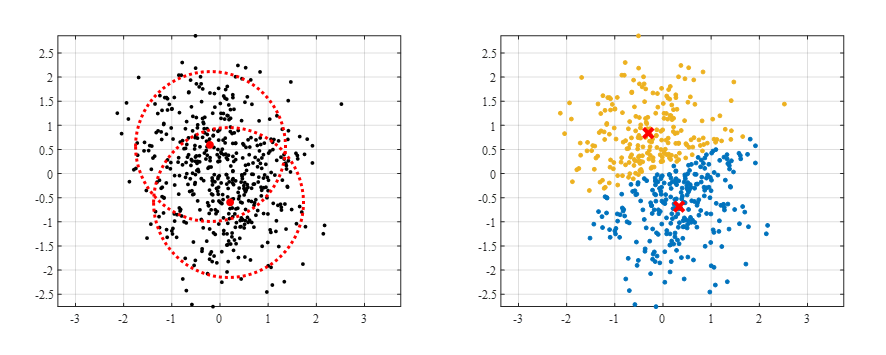
\includegraphics[width=15cm]{fig/hard_clustering.png}
 \caption{Grouping result of hard clustering by applying nearest neighbor rule.}
 \label{fig:hard_clustering}
\end{figure}

Clustering technology can be divided into two types: soft clustering and hard clustering. In hard clustering, each sample is accurately assigned to a group by applying the nearest neighbor rule. However, when samples from different sources are highly overlapped, it is difficult to tell which group the samples belong to in the overlap region.  In Fig.~\ref{fig:hard_clustering}, two sources produce samples with two-dimensional Gaussian distribution, and the mean values are represented as red dots. The Red Cross is the center of mass of the composition, and the color is shown in the figure Fig.~\ref{fig:hard_clustering}. The group classified by hard clustering in clustering.  Fig.~\ref{fig:hard_clustering} is the received symbol in BPSK modulation transmission of $U = 1 $user, and the SNR is relatively low. Therefore, the interference of channel noise makes it difficult to distinguish the two levels and reduces the accuracy of 
estimation.

Gaussian mixture model (GMM) is a method to realize soft clustering. It assumes that samples from different sources are Gaussian distributions with different parameters (mean and covariance). Therefore, the clustering problem is transformed into parameter optimization of Gaussian component in GMM. Expectation maximization (EM) algorithm \cite{em77} is usually used to find the parameters of Gaussian components in GMM. Since the channel noise is Gaussian distribution, the assumption of Gaussian component in GMM is suitable for the clustering of received symbols. In addition, as mentioned above, since the variance of each Gaussian component is equal to the variance of channel noise, and the probability of occurrence is equal, only the mean value of the component needs to be considered. For the signals received in GDMA system, the steps of EM cluster using GMM are as follows.

\begin{enumerate}[leftmargin=\leftmargin+\widthof{Prefix}]
\item[Step 1)] Initially set the occurrence probability $\text{Pr}(i)=2^{-mU}$ and the covariance matrix of Gaussian distribution is ${\bf \Sigma}_i = \sigma_w^2 {\bf I}_2$, where $\sigma_w^2$ is the variance of channel noise and ${\bf I}_2$ is a two-by-two unit matrix, for each component $i$ with $i \in \{1, 2, ..., 2^{mU}\}$.
\item[Step 2)] Proceed with k-means clustering and the resultant centroids are configured as the initial means of Gaussian components.
\item[Step 3)] Compute the soft assignment of each received symbol $r(n)$ by
\begin{equation}
 \text{Pr}(i|r(n)) = \frac{\mathcal{CN}(r(n)|\mu_i,{\bf \Sigma}_i)}{\sum_{j=1}^{2^{mU}}\mathcal{CN}(r(n)|\mu_j,{\bf \Sigma}_j)},
\end{equation}
where $i \in \{1,2,...,2^{mU}\}$ and $\mathcal{CN}$ denotes the PDF of complex Gaussian distribution.
\item[Step 4)] Derive the ML estimate of mean for component $i$ with
\begin{equation}
 \mu_i = \frac{1}{N_i} \sum_{n=1}^{N_t} r(n)\text{Pr}(i|r(n)),
\end{equation}
where $i \in \{1, 2, ..., 2^{mU}\}$ and $N_i=\sum_{n=1}^{N_t}\text{Pr}(i|r(n))$.
\item[Step 4)] Return to Step 3 until the means no longer change.
\end{enumerate}

The procedure of EM clustering is quite similar to that of the k-means algorithm, which needs the initialization of the parameters. Here we directly use the centroids derived from the k-means++ algorithm to be the initial means of Gaussian components in GMM, as stated in Step 2. After the EM clustering, the means of elements become the resultant centroids.

\section{Cluster-based Estimation Analysis and Design}

Cluster-based estimation can increase the efficiency of transmission, but it still has many problems. First, we analyzed how many samples are needed to achieve cluster reliability. Second, compared to \cite{yt19} only using the symmetric condition to judge whether it has correctly converged, we added more restrictions to increase algorithm security. Third, compared to the case where \cite{yt19} will plunge into fail loops to find correct convergence, we propose a method that can significantly reduce the number of iteration. Fourth, compared to the limitation \cite{yt19} of derivating channel coefficient, the algorithm we proposed can be applied in various cases.

\subsection{Clustering Sample Size Analysis}

The mean-square error (MSE) performances are simulated to evaluate the performance of cluster-based estimation applied to Rayleigh flat fading channels ,and the MSE is defined as

\begin{align}
\text{MSE}(h,\hat{h})=\frac{1}{2} | h,\hat{h} |^2  
\end{align}

where $h$ is the exact channel coefficient and $\hat{h}$ is the estimate of $h$. Note that the average energy of channel coefficient and transmitted signals are both normalized to one. The Cramer-Rao lower bound (CRLB), for the minimum variance unbiased (MVU) estimator using $N_t$ samples in the estimation, is also provided to evaluate the performance. Consider the observations when the signals are propagated through the channel with AWGN as
$r(n)=h+w(n),n=0,1,\cdots,N_t-1$.

\begin{figure}[b!]
 \centering
 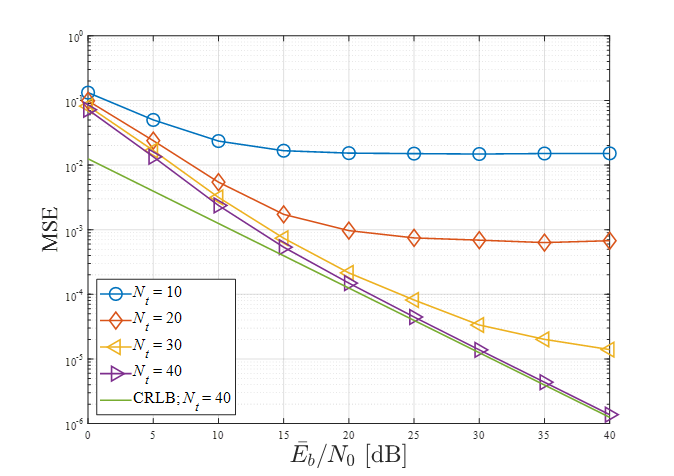
\includegraphics[width=15cm]{fig/sample_size_analysis1.png}
 \caption{MSE of estimated channel coefficient over AWGN channels.}
 \label{fig:sample_size_analysis1}
\end{figure}

,where $h$ is the parameter to be estimated and w(n) is AWGN with variance $\sigma_w^2$. The MVU estimator of h can be derived as 

\begin{align}
\hat{h} = \frac{1}{N_t} \sum_{n=0}^{N_t-1}r(n)  
\end{align}

and the variance of $\hat{h}$ is the CRLB written as

\begin{align}
\sigma^{2}_{h} = \frac{\sigma^{2}_{w}}{N_t}  
\end{align}

Assume that $U = 2$ and BPSK transmission, we changed the sample size arbitrarily. Observe the fig.\ref{fig:sample_size_analysis1} and find that the smaller the size, the earlier the error floor will occur. Because the number of samples is lack, some superimposed levels may not be generated and must lead to errors. We called it the worst case. In the following formula derivation, we derived the probability that the sample size will lead to the worst case.

Assume that $L=2^{mU}$ is the number of superimposed levels, $N_t$ is the number of clustering points and $A_i$ is the random variable that $i$-th superimposed level is empty where $i \in \{ 1, \ 2, \  \cdots, \  L \}$.

\begin{align}
& \text{Pr}{(A_i)} = {( \frac{L-1}{L} )}^{N_t} \nonumber \\
& \text{Pr}{(A_i \cap A_j)} = {( \frac{L-2}{L} )}^{N_t}, i \neq j  \ \nonumber \\
 & \quad \vdots \ \nonumber \\
& \text{Pr}{(A_i \cap A_j \cdots \cap A_r)} = {( \frac{1}{L} )}^{N_t}, i \neq j  \cdots \neq r \ 
\end{align}

\begin{align}
\text{Pr}{(\text{error})} &= \text{Pr}{(\text{at least one level is empty})} \ \nonumber \\
& = \text{Pr}{(A_i \cup A_j \cdots \cup A_r)} \ \nonumber \\
& = \text{C}^L_1 \ \text{Pr}{(A_i)} \ - \ \text{C}^L_2 \ \text{Pr}{(A_i \cup A_j)} \ + \ \text{C}^L_3 \ \text{Pr}{(A_i \cup A_j \cup A_j)} \ + \ \cdots  \nonumber \\
& + \ {(-1)}^{L-2} \ \text{C}^L_{L-1} \ \text{Pr}{(A_i \cup A_j \cup A_j \cdots)} \ \nonumber \\
& = \text{C}^L_1 \ {(\frac{L-1}{L})}^{N_t} \ - \ \text{C}^L_2 \ {(\frac{L-2}{L})}^{N_t} \ + \ \text{C}^L_3 \ {(\frac{L-1}{L})}^{N_t} \ + \ \cdots  + \ {(-1)}^{L-2} \ \text{C}^L_{L-1} \ {(\frac{1}{L})}^{N_t} \ 
\end{align}

\begin{figure}[H]
 \centering
 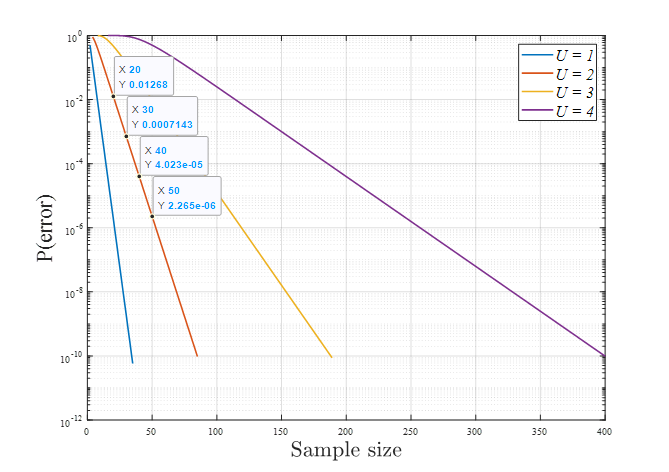
\includegraphics[width=15cm]{fig/sample_size_error_probability_analysis.png}
 \caption{The probability of worst case with BPSK transmission for different user $U$.}
 \label{fig:sample_size_error_rate}
\end{figure}

In Fig.\ref{fig:sample_size_error_rate}, derive the probability that superimposed levels is empty according to above equality. and list the following table.\ref{table:sample_size} that is probability with different clustering samples size. Fig.\ref{fig:sample_size_analysis} is the MSE of paired sample. Expect for $N_t=10$, sample size $N_t=20$ and $N_t=30$ both achieve the CRLB. 

\begin{table}[b!]
\caption{The probability that at least one superimposed level is empty for $L=4$.}
\begin{center}
 \begin{tabular}{ |c|c|c|c|c|c| }
 \hline
 Sample size & 10 & 20 & 30 & 40 & 50 \\
 \hline
 Pr\{error\}  & $0.2194$ & $0.01268$ & $7.143e^{-4}$ & $4.023e^{-5}$ & $2.265e^{-6}$ \\
 \hline
\end{tabular}
\end{center}
\label{table:sample_size}
\end{table}

\begin{figure}[t!]
 \centering
 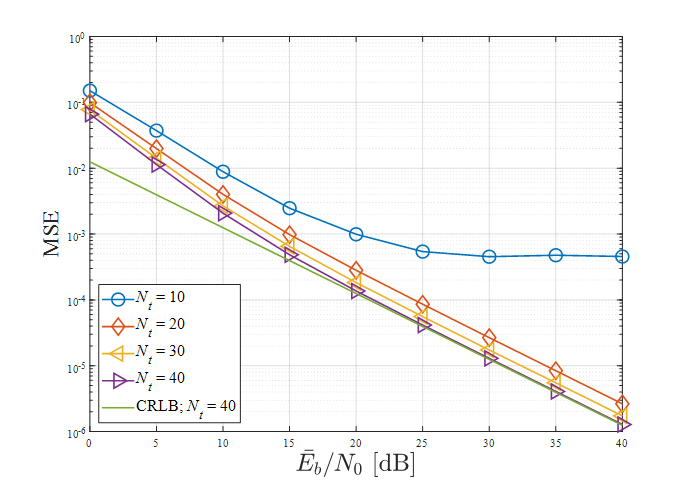
\includegraphics[width=15cm]{fig/sample_size_analysis.png}
 \caption{MSE of estimated channel coefficient with pair samples over AWGN channels.}
 \label{fig:sample_size_analysis}
\end{figure}


We can make up the problem according to the structure of modulation. Generate a sample with $\pi$ phase shift for BPSK transmission and create three copies of the received sample for QPSK transmission with $\frac{\pi}{2}, \ \pi ,\ \frac{3\pi}{2} $ phase shift respectively.

\subsection{Proposed Clustering Algorithm}

\begin{figure}[b!]
 \centering
 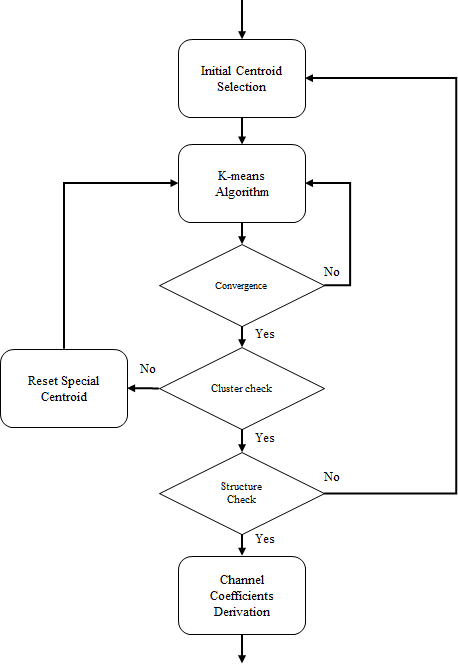
\includegraphics[width=10cm]{fig/flow_chart_proposed_clustering.png}
 \caption{The flow chart of proposed cluster-based channel estimation algorithm.}
 \label{fig:flow_chart_proposed_clustering}
\end{figure}

In the thesis \cite{yt19}, the main focus was on selecting good initial centroids, and a modified k-mean algorithm has also been proposed to make the initial centroid choosing better. In most of the clustering literature, it is mainly in the study of the initial centroids. Although the initial centroid selection is very important, it isn't easy to cluster correctly by completely modifying the initial selecting algorithm. We have come up with a different idea, not the study of initial centroids. The clustering algorithm in \cite{yt19} will re-execute if the symmetric condition is not met. The re-executed clusterings are independent of the previous one, resulting in inefficient or falling into a wrong loop. Hence, we came up with new ideas to make these re-executed clustering related to the last grouping and make them more efficient. Fig. \ref{fig:flow_chart_proposed_clustering} is the flow chart of proposed clustering algorithm. The cluster check is the algorithm to check whether convergence centroids are correct, roughly using the symmetric properties, group size, and group MSE. According to the cluster check, process the algorithm of resetting special centroids, which only reset the incorrect centroids. The structure check is the function to check centroids more accurately by using the superimposed level structure, and the channel coefficient derivation function is the novel algorithm different from \cite{yt19}.  The details of each flow block are described as the following subsection.


\subsubsection{Cluster Check}

In addition to selecting better initial centroids, we also change the algorithm after convergence. The fig.\ref{fig:cluster_check}-(a) is a cluster convergence case, but it does not conform to the superimposed levels symmetry condition. Thus, in the algorithm \cite{yt19}, the clustering algorithm would re-execute until the estimated centroids symmetry, but since each clustering algorithm is independent, it is possible to fall into a loop. Besides, even if it meets the symmetry condition, it could still be the wrong convergence.

Fig.\ref{fig:cluster_check}-(a), one case of convergence, it does not conform to the symmetric condition, but green centroids converge to the correct superimposed levels, where only red centroids do not. Hence, we can estimate whether those centroids converge correctly. Here, we use group MSE and group size to estimate centroids individually to check which centroid is reliable. 

Group MSE is the mean square error (MSE) of each cluster's centroid and its members. Under normal circumstances, group MSE should be similar to the noise variance. Therefore, if the group MSE is unusually large or small, this cluster is an error. Group MSE can be expressed as



\begin{align}
MSE_k = \sum^{N_{k}}_{i=0} \frac{{(r_{k,i} - C_k)}^2}{N_k}, \ k=1,2,\cdots,L
\end{align}

, where $N_k$ is the group size of $k$-th cluster, $C_k$ is the centroid of $k$-th cluster.


Group size is the number of members of each cluster. Under normal circumstances, the group size should be $\frac{N_t}{L}$ approximately and it can also be utensil to estimate. $N_k,k=1,2, \cdots, L$

We map group MSE or size into a reliability value for each centroid. If the value is smaller or larger than a threshold, label it a bad centroid. However, neither group MSE nor group size can not be entirely correct. We use them alternately until the estimated superimposed levels are the right structure.


\begin{figure}[t!]
 \centering
 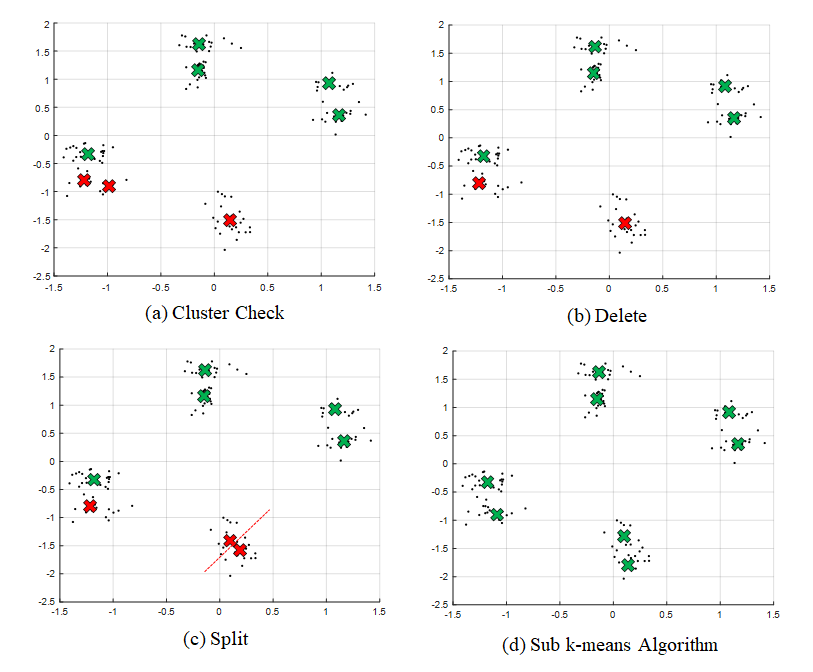
\includegraphics[width=14cm]{fig/cluster_check.png}
 \caption{An example of cluster check.}
 \label{fig:cluster_check}
\end{figure}

\begin{figure}[b!]
 \centering
 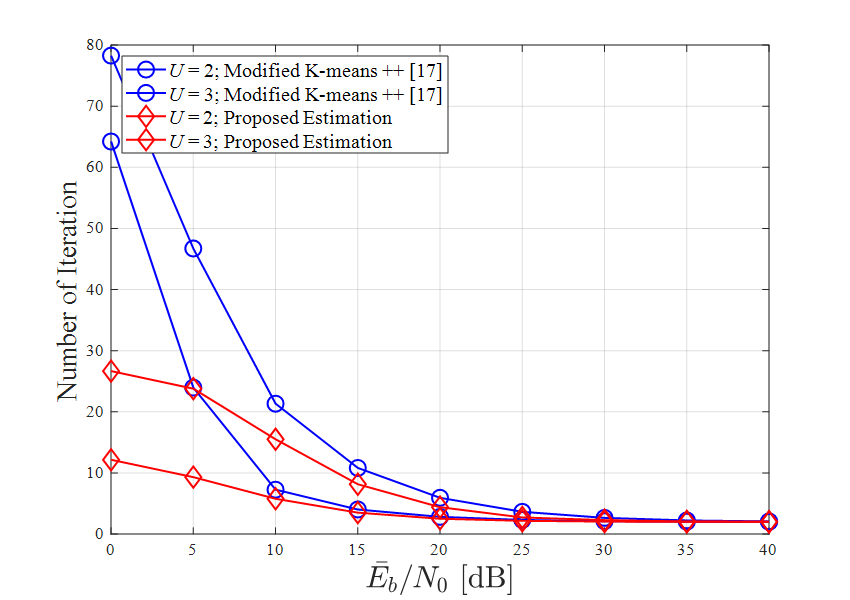
\includegraphics[width=14cm]{fig/channel_gain_iteration_128.png}
 \caption{The iteration number of estimated channel gain at $N_t=128$.}
 \label{fig:channel_gain_iteration_128}
\end{figure}


\subsubsection{Reset Special Centroid}

We obtain the bad centroids and good centroid after cluster check. It is only necessary to re-estimate the bad centroids that save a lot of operations and also ensure that the entire algorithm will not enter an error loop again.  If the reliability value is higher than the threshold, it indicated that the cluster group might miss centroids. In comparison, the value is less than the threshold indicated that the cluster group might have too many centroids. Firstly, delete the centroid with the smallest reliability value,which might be the redundancy centroids in fig.\ref{fig:cluster_check}-(b). Secondly, split the centroid with the most significant parameter, which cluster might miss centroids in fig.\ref{fig:cluster_check}-(c). The concept of splitting is same as LBG \cite{lbg80} algorithm where splitting from centroid$-q$ to get $q+\epsilon$ and $q-\epsilon$ with a perturbation vector $\epsilon$. Both add a random vector to the original centroid, splitting the centroid into two. 
Third, perform the k-mean algorithm on these reset centroids, so that all cluster parameters are close to convergence. Hence, the proposed clustering estimation is more efficient than the algorithm \cite{hsu2020uplink}, and we used the clustering iteration to compare two algorithms in fig.\ref{fig:channel_gain_iteration_128} at $N_t=128$, where iteration is the number of operations required for the clustering algorithm to converge to meet all structural constraints. The proposed clustering algorithm can greatly reduce iteration, especially in low SNR.


\begin{figure}[t!]
 \centering
 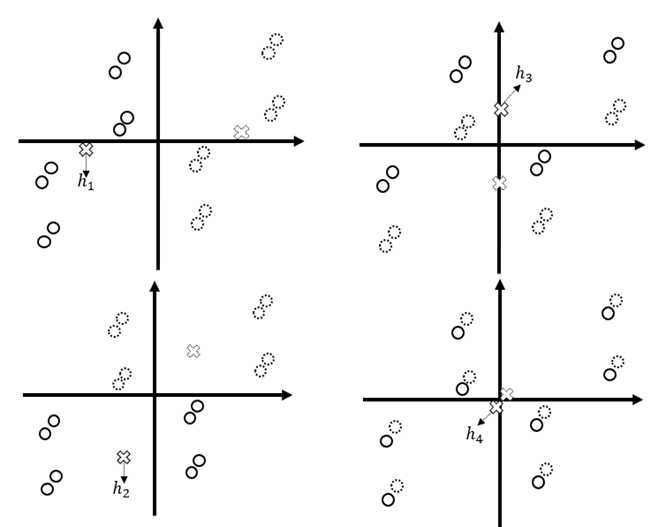
\includegraphics[width=15cm]{fig/structure_check.png}
 \caption{An example of structure check.}
 \label{fig:structure_check}
\end{figure}


\subsubsection{Structure Check}

After the above steps, the estimated superimposed levels can be correctly solved with a very high probability. This step is mainly to detect whether estimated centroids are entirely correct. Because this step requires a higher degree of complexity and will be used in the channel estimation, it is set in the final step detection. 
The fig.\ref{fig:derivation_channel_gain}-(a) is $U = 4$ BPSK transmission where $h_u$ is channel gain $u \in \{ 1,2,3,4 \}$ and the solid circles are the superimposed levels. We can find it has the following characteristics: dividing the superimposed level into two groups: solid circles and dotted circles in fig.\ref{fig:structure_check}. Because of half of the superimposed added with $h_u$ and the other half added with  $-h_u$, we can find the different symmetrical property with $h_u$ ; $u \in \{ 1,2,3,4 \}$ as the center. If it conforms to the structure, we can be very sure that the estimated centroids are correct. This structure will also be used in the next section, so there will be a more detailed discussion on how to implement it in the next section .\ref{section:Derivation of Channel Coefficients}.


\subsection{Derivation of Channel Coefficients}
\label{section:Derivation of Channel Coefficients}

We can classify the received symbols into $2^{mU}$ groups by the clustering techniques introduced in Sec.~\ref{s:clustering}, and the centroids of groups are the estimated superimposed levels. Recall that the fading coefficients are constant across a block of $N_t$ consecutive symbols, and the occurrence probabilities of superimposed levels are equally like in assumption. Using the derivation channel coefficient algorithm as following, we can further estimate the channel coefficients of $U$ users from the resultant centroids. In this section, ideal clustering that the centroids are exactly equal to superimposed levels is assumed to clearly illustrate the procedure. 

Before introducing the derivation of the channel coefficients algorithm, we must know how the superposition levels compose, and here we find the rules for its composition. As shown in the fig.\ref{fig:superimposed_levels_composation}, the levels are superimposed from channel gains $h_1$ to $h_4$ in sequence. The fig-(a) is the signal generated by $h_1$. The amplitude and phase of levels are the same as $h_1$ because of the BPSK transmission. The fig-(b) is the superimposed levels generated by $h_1$ and $h_2$. The superimposed levels are obtained by splitting $\pm$ $h_2$ from fig-(a), so the center of these two splitting groups is $\pm$ $h_2$. Fig-(c) is the superimposed levels generated by $h_1$ $h_2$ and $h_3$. Similarly, $\pm$ $h_3$ can be added to the four levels in fig-(b) separately, so it can be split into eight levels. Then, we can derive $2^{mU}$ superimposed levels from $U$ channel gains, which is the rule of superimposed signals. On the contrary, we can also derive channel gains from superimposed signals by the iterative process.
\\



\begin{figure}[t!]
 \centering
 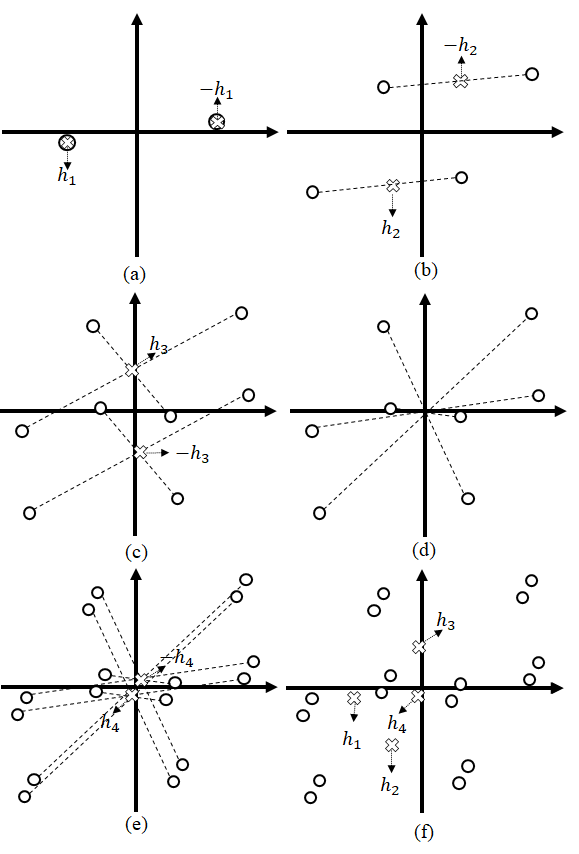
\includegraphics[width=15cm]{fig/superimposed_levels_composation.png}
 \caption{The steps to compose superimposed levels.}
 \label{fig:superimposed_levels_composation}
\end{figure}

From the rule of superimposed level composition,  channel gains can be solved one by one, which removes the level of information of solved gains. In this way, we only need to find the remaining channel gains, which can save a lot of operations. The steps of the derivation of channel coefficients is organized as follows.


\begin{enumerate}[leftmargin=\leftmargin+\widthof{Prefix}]
\item[Step 1)] Pair the $2^{mU}$ levels with the sum of each pair is equal to zero according to modulation.
\item[Step 2)] Group $2^{mU}$ levels into $2m$ groups, each signal of groups are not in the same pair, and derive the centroids of each group, where $m$ is the modulation order.
\item[Step 3)] Return to Step 2 until each group is symmetrical with their centroids.
\item[Step 4)] Derive the channel coefficient that is the group centroid.
\item[Step 5)] Shift $2m$ groups to the original point.
\item[Step 6)] Return to Step 1 and $U=U-1$ until all coefficients are derived.
\end{enumerate}

Fig.\ref{fig:derivation_channel_gain} is process of derivation of channel coefficient. The first step is to pair the centroids with each pair's sum equal to zero in fig-(b).  Step 2 is the brute force method for getting all compositions, and there are $2^{2^{mU}-1}$ combinations in total, but only $2mU$ combinations are correct that is an exponential operation according to $U$ user. Fig-(b) is the false case, and fig-(c) is the correct case. Then, deposit the derived estimated channel gain, which is the centroid of the two groups. We only need to derive the remaining channel gains. According to modulation order $m$, the group number is also different. In step 5, shift the symmetrical groups into the original point and average the pair levels, which can reduce $2^{mU}$ levels into $2^{mU-1}$ levels as fig-(e).


\begin{figure}[t!]
 \centering
 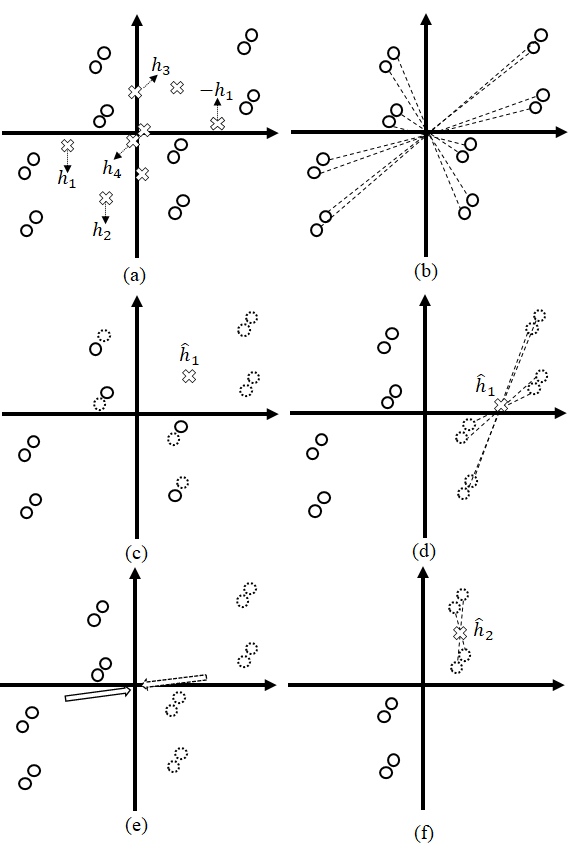
\includegraphics[width=15cm]{fig/derivation_channel_gain.png}
 \caption{The steps of derivation of channel coefficients.}
 \label{fig:derivation_channel_gain}
\end{figure}

The fig.\ref{fig:derivation_channel_gain} is an example of $U=4$, BPSK transmission for deriving channel gains. The first step is to pair all levels. After pairing, group levels into two groups with the restrictions, as shown in (c), it is obvious that the levels in fig-(c) are not symmetrical with their centroids. Therefore, return to step 2 and generate two groups again until it meets the symmetrical condition, as shown in fig-(d). Then, shift the corresponding groups to the original point, and search the remaining levels for deriving rest channel gains.

Compared with the previous geometric method, the novel method does not limit the size of $U$, even if the modulation is different. In terms of implementation, the method only needs a loop to make it work. Compared with the previous implementation complexity, which has been improved a lot. However, in terms of computational complexity, especially in step 2, it will grow exponentially with the $U$ users, which might be improved in future work.

\begin{figure}[t!]
 \centering
 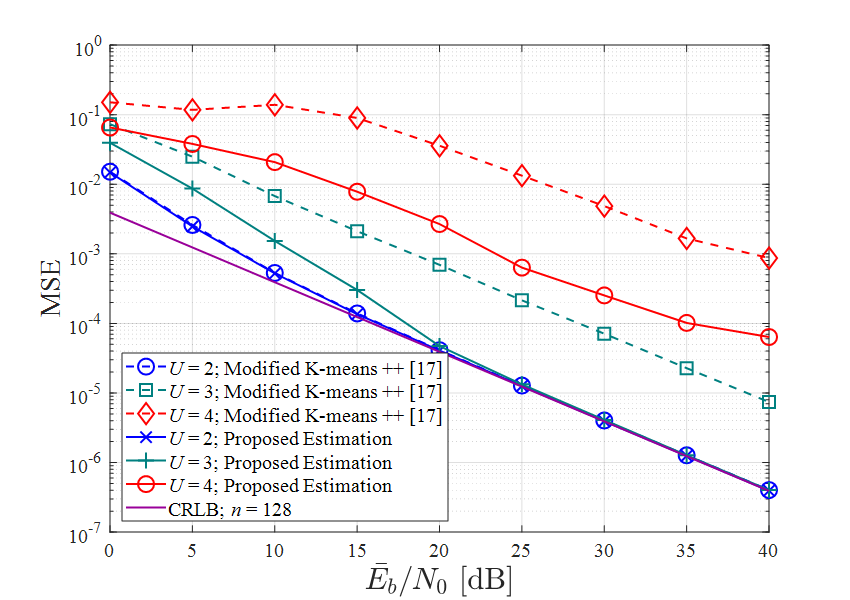
\includegraphics[width=14cm]{fig/channel_gain_mse_128.png}
 \caption{The MSE of estimated channel gain at $N_t=128$. GMM is used.}
 \label{fig:channel_gain_mse_128}
\end{figure}

\begin{figure}[t!]
 \centering
 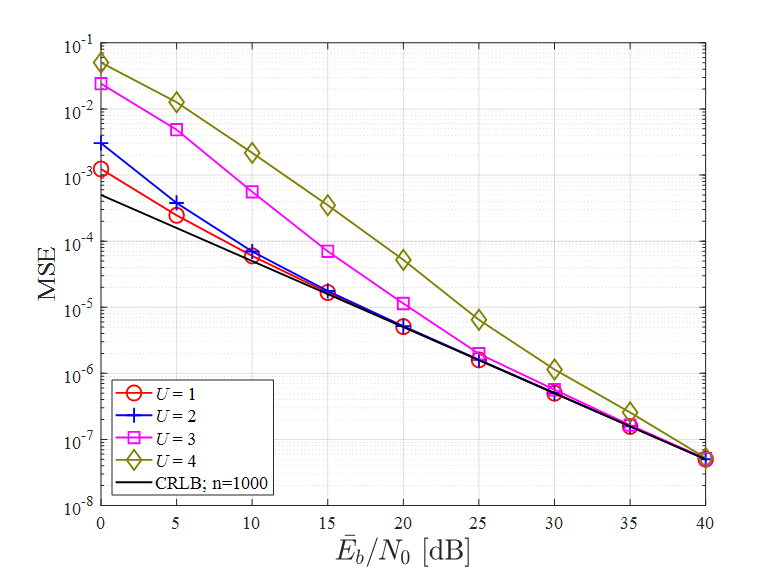
\includegraphics[width=14cm]{fig/channel_gain_mse_1000.png}
 \caption{The MSE of estimated channel gain at $N_t=1000$. GMM is used.}
 \label{fig:channel_gain_mse_100}
\end{figure}


Fig.\ref{fig:channel_gain_mse_128} is the MSE performance of estimated channel gain in a different algorithm, where we compare the navel algorithm with the previous algorithm in \cite{hsu2020uplink}. Assume received samples $N_t=128$. When $U=3$, the proposed algorithm can approach CR bound. Compared with paper \cite{hsu2020uplink}, the effect is excellent, and when $U=4$, it is also good. Because there are too few samples, there is no way to ensure that all superimposed levels are reliable, so it still can not approach CRLB. When the number of samples is increased, we can solve this problem. Fig.\ref{fig:channel_gain_mse_100} is the MSE of $N_t=1000$, When high SNR, $U=4$ can still be close to CRLB. As long as the sample is enough, the proposed clustering algorithm can achieve CRLB.


\section{Resolving Phase Ambiguity}
\label{s:ambiguity}

Although we can have the estimates of channel coefficients through the clustering, there is still an uncertain phase ambiguity due to the estimation using signals that carry messages. An easy way to remove the uncertainty(ambiguity) is to differentially encode the message. However, the differential encoding results in a loss of error performance because of error propagation. Hence, several methods like differential encoder, BCJR decoder, joint decoding, and NBC are introduced to solve phase ambiguity in the thesis \cite{yt19}. Here, we introduce a novel method called $ Q $-section NBC using the polar code structure. In a single carrier system, only need NBC to resolve the phase ambiguity but can not in $Q$ multiple carrier system since there are $Q$ phase ambiguities in a codeword. In this section, we introduce differential encoder, NBC, Q-section NBC in sequence.

\subsection{Differential Encoding}

Differentially encoded (DE) modulation uses the difference between symbols to carry a message. In the transmission of PSK, a message is embedded in the difference of phases between two consecutive symbols, and coherent detection can still be applied, resulting in differentially encoded coherently detected PSK (DE-PSK). Therefore, the phase offset resulted from uncertain ambiguity in blind estimation will not affect the detection of data in DE-PSK transmissions. The block diagram of the DE-BPSK scheme is provided in Fig.~\ref{fig:de_bpsk_enc}.

\begin{figure}[t!]
 \centering
 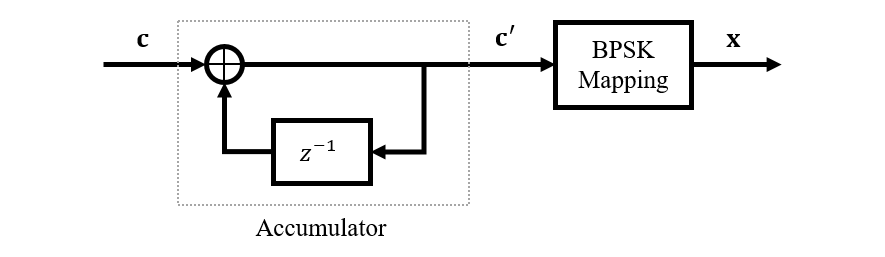
\includegraphics[width=15cm]{fig/de_bpsk_enc.png}
 \caption{Modulation scheme for DE-BPSK transmission.}
 \label{fig:de_bpsk_enc}
\end{figure}

\subsection{Noncoherent Block-Coded Modulation}

In \cite{nbc05}, a novel block-coded modulation (BCM) scheme with noncoherent detection called noncoherent block-coded MPSK (NBC-MPSK) was proposed. The ambiguity can be easily removed without applying differential encoding by partitioning the code space as long as the generator matrix of a linear block code containing an all-one row.

The original code space $C'$ is divided into $C'=\{C, C \oplus \bf 1\}$, where $\bf 1$ is an all-one vector, and the generator matrix $\bf G$ of $C$ is found by removing the all-one row in the generator matrix of $C'$. We only select the codewords from $C$ to be transmitted, i.e., encode the message with $\bf G$, resulting in a rate loss of one bit. At the receiver side, if the signal is BPSK-modulated, the codeword $\bf c'$ corresponding to the received signal would be $\bf c$ or ${\bf c} \oplus {\bf 1}$ due to an uncertain phase ambiguity of $180^{\circ}$ where $\bf c$ is the transmitted codeword in $C$. To remove the uncertain ambiguity, we just need to detect whether the decoded codeword $\tilde{\bf c}$ is in $C$ or not and the resultant codeword is
\begin{equation}
 \hat{\bf c} =
  \begin{dcases}
   \ \tilde{\bf c}, & \text{if } \tilde{\bf c} \in C \\
   \ \tilde{\bf c} \oplus {\bf 1}, & \text{if } \tilde{\bf c} \not\in C
  \end{dcases}
\label{equ:space_identification}
\end{equation}

\begin{figure}[t!]
 \centering
 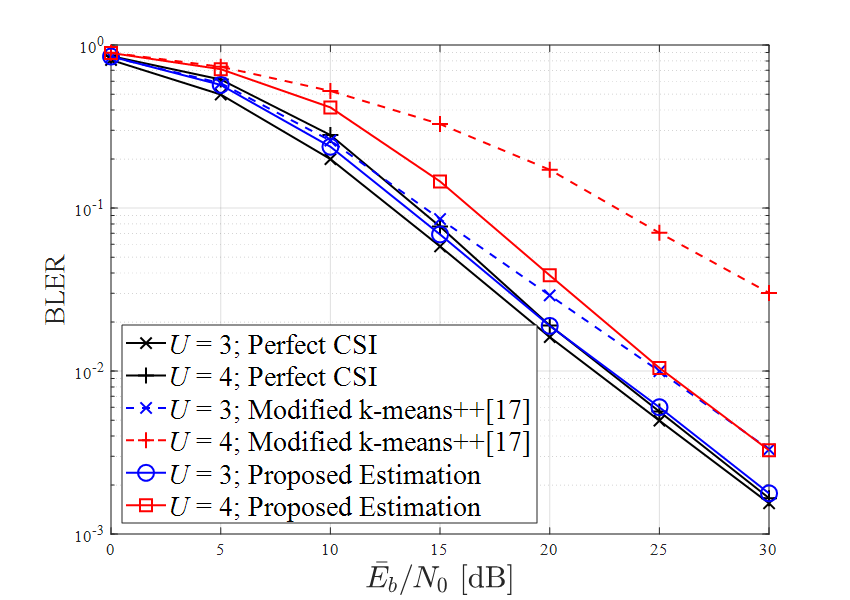
\includegraphics[width=15cm]{fig/bler_polar_channel_estimation.png}
 \caption{BLER performances for a (128,64) Polar-coded GDMA system over
quasi-static Rayleigh flat-fading single carrier channels. NBC and GMM are both used.}
 \label{fig:bler_polar_channel_estimation}
\end{figure}


For a higher-order modulation scheme, the multi-level coding in BCM can be decoded by multi-stage decoding, as shown in \cite{nbc05}. The code space identification in (\ref{equ:space_identification}) can be implemented by checking the number of satisfied parity-check equations. However, the bit errors after decoding might result in erroneous identification and redundant bit-flipping. 

We consider the (128, 64) Polar-coded and the BPSK modulated GDMA system over quasi-static Rayleigh fading channels based on perfect timing. The block error rate (BLER) performances from the simulation are provided in fig. \ref{fig:bler_polar_channel_estimation}. Successive cancellation list (SCL) decoding is used where the list size is 32. Set n = 128. In this case, the phase ambiguity is resolved via NBC. For $U = 3$ and $U = 4$, the BLER using proposed estimation algorithm is obviously better than algorithm in \cite{hsu2020uplink}.

\subsection{Section Noncoherent Block-Coded Modulation}

Consider a codeword transmits into a multi-carrier system and passes through a $Q$ multi-carrier system. Since the cluster-based channel estimation still has the phase ambiguity problem in each sub-carrier channel gains, the received codeword might be split into $Q$ segments. For example, codeword 0000 passes through a two multi-carrier system. The received codeword may be 0011, 1100, 0000, 1111 , and the Q-section NBC was proposed to solve this problem.

In Q-section NBC, the original code space $C'$ is divided into $C'=\{C, C \oplus {\bf{v_1}}, C \oplus {\bf{v_2}}, \cdots, C \oplus {\bf{v_Q}} \}$, where ${\bf{v_i}}, i \in \{ 1, \cdots, Q \}$ are the vectors for splitting the code space, and the generator matrix $\bf G$ of $C$ is found by removing all control vectors in the generator matrix of $C'$. We only select the codewords from $C$ to be transmitted, i.e., encode the message with $\bf G$, which results in a rate loss of $Q$ bit. The control vectors $v_i$ are designed according to multi carrier mapping as following matrix ${\bf V} = {[{\bf{v_1}} \ {\bf{v_2}} \ \cdots \ {\bf{v_Q}}]}^{\text{T}}$.

Assume that the code length $N=2^n$, the section $Q=2^q$, ${\bf{v_0}}$ is an all-one vector. Firstly, generate the control vectors $v_i, i \in \{ 1 \ , 2 , \cdots , q-1 \}$, and the ${\bf{v_i}}$ is described as \ref{equ:v_i}. Then, utensil $j$ control vectors ${\bf{v_i}}$ to generate remaining vectors, where $j \in \{  1, \ , 2 , \cdots , q \}$ is the combination number. Finally, we would derive $Q$ vectors, where $Q=2^q=1+C^q_1+C^q_2+\cdots+C^q_q$.




\begin{align}
{\bf{v_i}} = {( \underbrace{1 \cdots 1}_{2^{n-i}} \ \underbrace{0 \cdots 0}_{2^{n-i}} \ \underbrace{1 \cdots 1}_{2^{n-i}} \ \underbrace{0 \cdots 0}_{2^{n-i}})}; i \in \{ 1, \ 2, \cdots , q  \}.
\label{equ:v_i}
\end{align}

The equation.\ref{equ:section_NBC_1} is an example for $N=8$ and $Q=4$. Generate ${\bf{v_1}}$ and ${\bf{v_2}}$ according to section $q=2$, and derive ${\bf{v_3}}={\bf{v_1}} \oplus {\bf{v_2}}$.  
\begin{equation}
{\bf V}= {
\left[ \begin{array}{ccc}
{\bf{v_0}} \\
{\bf{v_1}} \\
{\bf{v_2}} \\
{\bf{v_3}}
\end{array} 
\right ]}= {
\left[ \begin{array}{ccc} 
\bf v_0 \\
\bf  v_1 \\
\bf  v_2 \\
\bf  v_1 \oplus v_2
\end{array} 
\right ]} 
= {
\left[ \begin{array}{cccccccc}
1 & 1 & 1 & 1 & 1 & 1 & 1 & 1\\
1 & 1 & 1 & 1 & 0 & 0 & 0 & 0\\
1 & 1 & 0 & 0 & 1 & 1 & 0 & 0\\
1 & 1 & 0 & 0 & 0 & 0 & 0 & 0
\end{array}
\right ]}; \ Q=4; \ N=8
\label{equ:section_NBC_1}
\end{equation}


The equation.\ref{equ:section_NBC_2} is an example for $N=16$ and $Q=8$. Generate $\bf v_0, \ v_1, \ v_2, \ v_3$ according to section $q=4$. Then, derive $\bf v_4, v_5, v_6$, which is combined by two vectors and $\bf v_7$ is combined by three vectors. 
\begin{equation}
{\bf V} = {
\left[ \begin{array}{ccc}

\bf v_0 \\
\bf v_1 \\
\bf v_2 \\
\bf v_3 \\
\bf v_1 \oplus v_2 \\
\bf v_1 \oplus v_3 \\
\bf v_2 \oplus v_3 \\
\bf v_1 \oplus v_2 \oplus v_3
\end{array} 
\right ]} = {
\left[ \begin{array}{cccccccccccccccc}
1 & 1 & 1 & 1 & 1 & 1 & 1 & 1 & 1 & 1 & 1 & 1 & 1 & 1 & 1 & 1\\
1 & 1 & 1 & 1 & 1 & 1 & 1 & 1 & 0 & 0 & 0 & 0 & 0 & 0 & 0 & 0\\
1 & 1 & 1 & 1 & 0 & 0 & 0 & 0 & 1 & 1 & 1 & 1 & 0 & 0 & 0 & 0\\
1 & 1 & 0 & 0 & 1 & 1 & 0 & 0 & 1 & 1 & 0 & 0 & 1 & 1 & 0 & 0\\
1 & 1 & 1 & 1 & 0 & 0 & 0 & 0 & 0 & 0 & 0 & 0 & 0 & 0 & 0 & 0\\
1 & 1 & 0 & 0 & 1 & 1 & 0 & 0 & 0 & 0 & 0 & 0 & 0 & 0 & 0 & 0\\
1 & 1 & 0 & 0 & 0 & 0 & 0 & 0 & 1 & 1 & 0 & 0 & 0 & 0 & 0 & 0\\
1 & 1 & 0 & 0 & 0 & 0 & 0 & 0 & 0 & 0 & 0 & 0 & 0 & 0 & 0 & 0
\end{array}
\right ]}; \ Q=8; \ N=16
\label{equ:section_NBC_2}
\end{equation}

Matrix.\ref{equ:section_polar_construction} is the polar code construction for $N=16$. The section NBC control vector $\bf{v_i}$ is the $\frac{N}{Q} \cdot i$-th row of polar code structure, $i = 1 , \cdots, Q$. If $\bf{v_i}$ is information bits for polar code,  we do not put message on it. Since the ambiguity phase shift, these bits are used for control phase, e.g., they are not message bits. If $\bf {v_i}$ is frozen bits for polar code, different from conventional SCL decoding, we can not feedback $0$ for message passing. Since these bits are also used for control phase, it might be $0$ or $1$ randomly. Here, we use list to record these frozen bits for fetching up this issue. \ref{fig:bler_gdma_ofdm_polar_sectionNBC} is the BLER performance for 16 phase ambiguity polar coded OFDM system. where SCD SCL-32 is used.



\begin{equation}
{\begin{array}{ccc}
\\ \bf v_1 \oplus v_2 \oplus v_3 & \longrightarrow \\
\\ \bf v_1 \oplus v_2 & \longrightarrow \\
\\ \bf v_1 \oplus v_3 & \longrightarrow \\
\\ \bf v_1  & \longrightarrow \\
\\ \bf v_2 \oplus v_3 & \longrightarrow \\
\\ \bf v_2 & \longrightarrow \\
\\ \bf v_3 & \longrightarrow \\
\\ \bf v_0 & \longrightarrow \\
\end{array} 
} 
{\left[ \begin{array}{cccccccccccccccc}
1 & 0 & 0 & 0 & 0 & 0 & 0 & 0 & 0 & 0 & 0 & 0 & 0 & 0 & 0 & 0\\
1 & 1 & 0 & 0 & 0 & 0 & 0 & 0 & 0 & 0 & 0 & 0 & 0 & 0 & 0 & 0\\
1 & 0 & 1 & 0 & 0 & 0 & 0 & 0 & 0 & 0 & 0 & 0 & 0 & 0 & 0 & 0\\
1 & 1 & 1 & 1 & 0 & 0 & 0 & 0 & 0 & 0 & 0 & 0 & 0 & 0 & 0 & 0\\
1 & 0 & 0 & 1 & 0 & 0 & 0 & 0 & 0 & 0 & 0 & 0 & 0 & 0 & 0 & 0\\
1 & 1 & 0 & 1 & 1 & 0 & 0 & 0 & 0 & 0 & 0 & 0 & 0 & 0 & 0 & 0\\
1 & 0 & 1 & 0 & 1 & 0 & 0 & 0 & 0 & 0 & 0 & 0 & 0 & 0 & 0 & 0\\
1 & 1 & 1 & 1 & 1 & 1 & 1 & 1 & 0 & 0 & 0 & 0 & 0 & 0 & 0 & 0\\
1 & 0 & 0 & 0 & 0 & 0 & 0 & 0 & 1 & 0 & 0 & 0 & 0 & 0 & 0 & 0\\
1 & 1 & 0 & 0 & 0 & 0 & 0 & 0 & 1 & 1 & 0 & 0 & 0 & 0 & 0 & 0\\
1 & 0 & 1 & 0 & 0 & 0 & 0 & 0 & 1 & 0 & 1 & 0 & 0 & 0 & 0 & 0\\
1 & 1 & 1 & 1 & 0 & 0 & 0 & 0 & 1 & 1 & 1 & 1 & 0 & 0 & 0 & 0\\
1 & 0 & 0 & 0 & 1 & 0 & 0 & 0 & 1 & 0 & 0 & 0 & 1 & 0 & 0 & 0\\
1 & 1 & 0 & 0 & 1 & 1 & 0 & 0 & 1 & 1 & 0 & 0 & 1 & 1 & 0 & 0\\
1 & 0 & 1 & 0 & 1 & 0 & 1 & 0 & 1 & 0 & 1 & 0 & 1 & 0 & 1 & 0\\
1 & 1 & 1 & 1 & 1 & 1 & 1 & 1 & 1 & 1 & 1 & 1 & 1 & 1 & 1 & 1\\
\end{array}
\right ]}
\label{equ:section_polar_construction}
\end{equation}


\begin{figure}[t!]
 \centering
 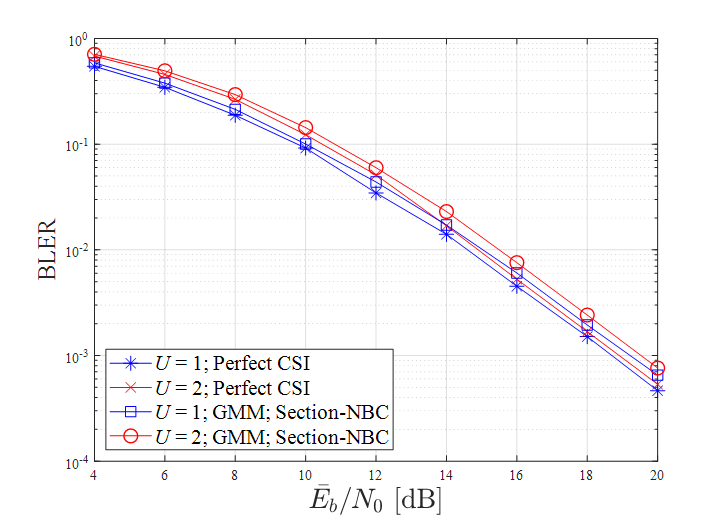
\includegraphics[width=15cm]{fig/bler_gdma_ofdm_polar_sectionNBC.png}
 \caption{BLER performances of Polar-coded GDMA OFDM systems over quasi-static Rayleigh flat-fading channels with 16-subcarrier.}
 \label{fig:bler_gdma_ofdm_polar_sectionNBC}
\end{figure}





\chapter{A Random Access Scheme based on Gain Division Multiple Access}
\label{c:rach_gdma}

Recently, random access protocol has not only caused the rise of satellite communication, but also caused the application of Internet of things (IOT) and machine to machine. In this chapter, we will implement a random access scheme based on gain division multiple access. Assumed that the system is UL transmission, and numerous devices use the same channel resources to transfer in a common evolved NodeB (eNB). Unlike ordinary random access, when a packet collision occurs, the eNB does not directly feedback HARQ (hybrid automatic repeat request), but multiuser detection (MUD) using the concept of GDMA. Then, we will introduce RACH and Grant to discuss various situations in our system further. In the second section, we will present the RA system more clearly and derive the ALOHA system's throughput. In the third section, we will introduce the random access orthogonal-frequency division multiplexing gain division multiple access (RA-OFDM-GDMA) system. Discuss the different cases of the MUD based on the variation of RACH and Grant. Then, add a preamble sequence to execute synchronization and hybrid channel gain estimation.


\section{Introduction of RACH and Grant}

RACH stands for Random access channel, which is the first message from UE to eNB when power on it. RACH is used in many places, e.g., achieve uplink synchronization between user equipment(UE) and eNB, obtain the resource for RRC connection request, etc. From the perspective of eNB, the UE signal is almost in a random fashion, e.g., casual time, random frequency, arbitrary identification. 

Before UE decides to send RACH signals (RACH preamble), many preconditions are called “Power-On to PRACH”. The steps of power-on to PRACH are described as :

\begin{enumerate}[leftmargin=\leftmargin+\widthof{Prefix}]
\item[Step 1)] UE is off.
\item[Step 2)] Power On UE.
\item[Step 3)] UE tune to a specific frequency.
\item[Step 4)] Time and Frame synchronization (PSS SSS decode).
\item[Step 5)] Physical Cell ID(PCI) , PBCH detection.
\item[Step 6)] Initial RACH process.
\end{enumerate}

, where Primary Sync Sequence(PSS) provides Radio Frame Boundary using preamble sequence and Secondary Sync Sequence (SSS) provides Subframe Boundary using correlation windows.

There are two type of RACH process : contention-based and contention-free. 

The steps of Contention-base RACH in 5G NR are summarized below.
\begin{enumerate}[leftmargin=\leftmargin+\widthof{Prefix}]
\item[Step 1)] Preamble transmission : The preamble is assigned by the UE. The UE selects one of the 64 preambles from the system information provided by the eNB to compete (Msg1).
\item[Step 2)]Random Access Request : If a collision occurs, perform a back of. If successful, the eNB knows the UE information.
\item[Step 3)]Radio Resource Control Connection Request : Reply Random Access response to UE, including Timing Advance and UL grant.
\item[Step 4)] RRC Connection Setup : After receiving the RAR, the UE will upload the ID with the UE information in the UL grant. If no other UE uses the same preamble in Msg1, the UE will compete for the channel resources of the RAP.
\end{enumerate}


The steps of Contention-free are summarized below.
\begin{enumerate}[leftmargin=\leftmargin+\widthof{Prefix}]
\item[Step 1)] Preamble Allocation : The preamble is assigned by the eNB.
\item[Step 2)] Preamble Transmission : The eNB knows the UE information.
\item[Step 3)] 5)	Radio Resource Control Connection Request : Reply Random Access response to UE, including Timing Advance and UL grant.
\end{enumerate}

\begin{figure}[t!]
 \centering
 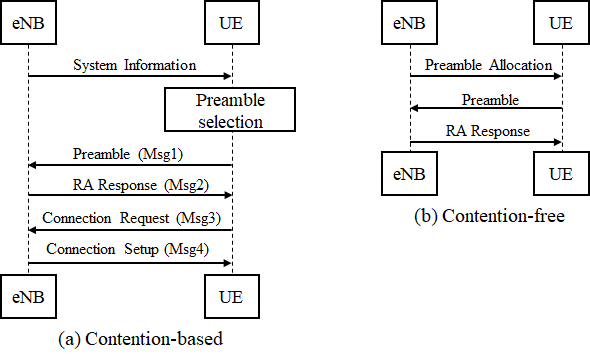
\includegraphics[width=10cm]{fig/RACH_contention_based_free.png}
 \caption{Two type of RACH process.}
 \label{fig:RACH_contention}
\end{figure}

The paper\cite{shahab2019grant} classified that RACH-based Grant-base, RACH-based Grant-free, RACH-free Grant-free system, where Grant means whether the number of users choosing a particular frequency sub-band is random. Users transmit data on an “arrive and go” basis (grant-free), or the receiver already allocates some specific number of users a particular subband. The transmission is scheduling(grant-based), e.g., users are aligned/connected in typical cellular communication.

\section{Introduction of Random Access System}

\begin{figure}[b!]
 \centering
 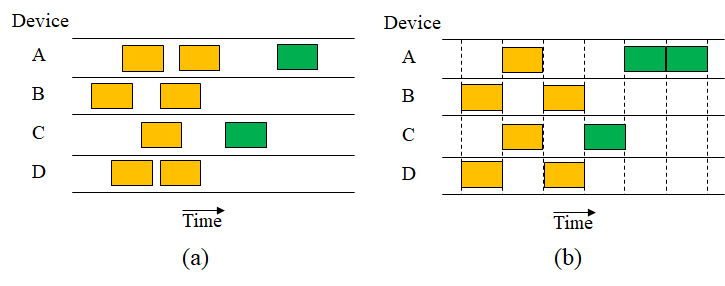
\includegraphics[width=10cm]{fig/RACH_slotted_unslotted.png}
 \caption{(a) An unslotted ALOHA system. (b) A slotted ALOHA system.}
 \label{fig:RACH_slotted_unslotted}
\end{figure}

\begin{figure}[t!]
 \centering
 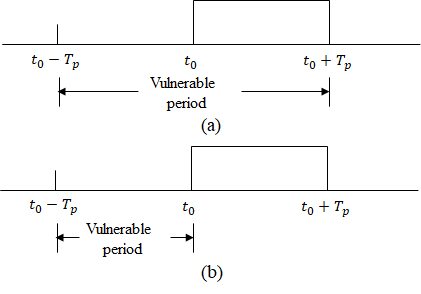
\includegraphics[width=10cm]{fig/RACH_vulnerable.png}
 \caption{(a) The vulnerable period for unslotted system. (b) The vulnerable period for slotted system.}
 \label{fig:RACH_vulnerable}
\end{figure}

In this section, we consider a multiuser communication system in which users transmit information in packets with common channel resource. In contrast to the CDMA or TDMA, the transmission would not be scheduled in advance. In conventional MA, the channel resource would be wasted during the period that device is granted to access, but it has nothing to say. If the number of device is massive, these MA will waste more resources. However, this is just a situation where random access techniques tend to become efficient. The access methods described below are basically random because packets are generated according to some statistical models. Users access the channel when they have one or more packets overlap in time, they collide, and, hence, a conflict results. If more than one frame are transmitted, they interfere with each other and are lost. If ACK not received within the timeout, then a user picks random backoff time. An ALOHA scheme \cite{abramson1970aloha} was originally analyzed for random access system at the University of Hawaii in 1970, which provides access to a common communication channel from multiple independent packet transmitters by the simplest of all mechanisms. The ALOHA system can be classified into two types in fig by slotted(RACH).\ref{fig:RACH_slotted_unslotted}.

We assume that the start time of packets that are transmitted is a Poisson point process having an average rate of $\lambda$ packets/s at the receiver.
Let $T_s$ denote the time duration of a packet. Then, the normalized channel traffic $G$, is defined as $G = \lambda T_s$ packets/duration.
For a time duration, the probability  of there being k transmission 


For the unslotted ALOHA system, the packets are transmitted at any arbitrary time, e.g., a user transmits whenever it has data to transmit. A successful transmission probability is a probability that there is no additional packet transmission in the vulnerable period. The vulnerable period of unslotted is $2T_ps$, as shown in fig\ref{fig:RACH_vulnerable}. If there are two or more packets arrived at the vulnerable period, the packets will collide. For the slotted ALOHA system, the packets are transmitted in the time slots, which can also be regarded as the RACH-based system, which vulnerable period is $T_s$. The throughput of the two systems are described as:


	
The throughput of unslotted ALOHA system:	
\begin{align}
S &= G \cdot Pr \{ \text{no collision} \}  \nonumber \\
  &= G \cdot Pr \{ \text{0 tansmissions in 2} \ T_p \} \nonumber \\
  &= G \cdot \frac{{2G}^{0}}{0! \cdot e^{-2G}} \nonumber \\
  &= G \cdot e^{-2G}
\end{align}

The throughput of slotted ALOHA system:	
\begin{align}
S &= G \cdot Pr \{ \text{no collision} \}  \nonumber \\
  &= G \cdot Pr \{ \text{0 tansmissions in 1} \  T_p \} \nonumber \\
  &= G \cdot \frac{{G}^{0}}{0! \cdot e^{-G}} \nonumber \\
  &= G \cdot e^{-G}
\end{align}

\begin{figure}[t!]
 \centering
 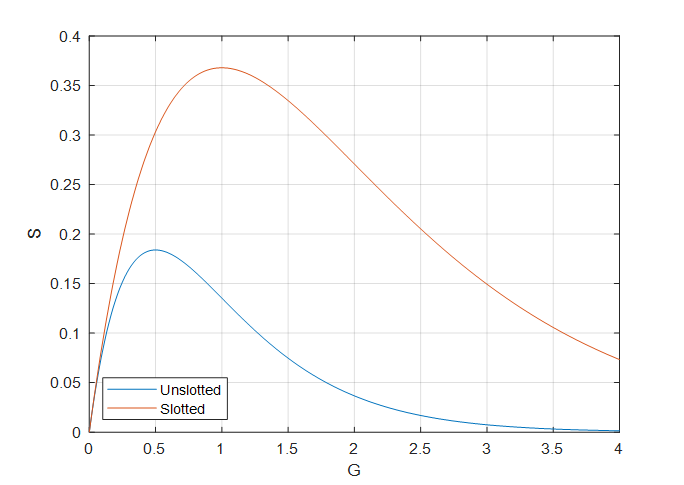
\includegraphics[width=15cm]{fig/RACH_ALOHA_throughput.png}
 \caption{The throughput of ALOHA system.}
 \label{fig:RACH_ALOHA_throughput}
\end{figure}

Fig. \ref{fig:RACH_ALOHA_throughput} is the throughput of ALOHA system. For unslotted system, $G = 0.5$ has the largest throughput $S \approx 0.1839 $, and for slotted system, $G = 1$ has the largest throughput $S \approx 0.3679$.

Based on the conventional ALOHA scheme, several random access protocols were developed \cite{alohaspread2005} \cite{massey1981collision} \cite{slottedalohathroughput} \cite{unslottedCDMA}. Most of them used more channel resources to avoid collisions, e.g.,  Spread-ALOHA will increase the spectrum usages, carrier sensing multiple access (CSMA) will increase the carrier usages, etc. Some researches are to resolve collision by contention tree or contention stack based on ALOHA re-transmission. However, there are more device connections, fewer channel resources, and low latency in modern communication systems. We introduced a novel RA scheme to resolve the collisions without additional channel resources, which is a similar GDMA concept.

\section{System Model}



\subsection{OFDM-GDMA system}

The proposed scheme can be applied to an orthogonal-frequency division multiplexing (OFDM) system.   For each $i \in \{0, 1, ...,N/(mQ)-1\}$, the subblock $[x_u(iQ+1), ..., x_u((i+1)Q)]$ is input into the $Q$-point inverse fast Fourier transform (IFFT) device to obtain the time domain signal. A cyclic prefix (CP) is inserted so as to avoid inter-symbol interference (ISI) and inter-carrier interference (ICI). On the receiver side, following CP removal and the $Q$-point FFT process, the frequency domain signal is then sent to the multi-level receiver.  Let $H_u(j)$ be the channel gain between user-$u$ and the receiver over the $j$-th sub-channel for $j \in \{1,...,Q\}$.  For the frequency domain signal, the component in the $j$-th sub-channel is
\begin{equation}
 r(iQ+j) = \sum_{u=1}^{U} H_u(j) x_{u}(iQ+j) + W(iQ+j),
\end{equation}
where $W(iQ+j)$ is the AWGN. The clustering-based channel estimation is performed for each of the sub-channels separately.

\subsection{Doppler-effect and unknown timing drift}
\label{s:Doppler-effect and unknown timing drift}

\begin{figure}[t!]
 \centering
 \includegraphics[width=15cm]{fig/OFDM_GDMA_doppler_timedrift.png}
 \caption{BLER performances for a (1008,504) LDPC-coded OFDM-GDMA
system where U = 2 users over frequency-selective Rayleigh fading channels.}
 \label{fig:OFDM_GDMA_doppler_timedrift}
\end{figure}

We now consider applying the proposed scheme to time-variant channels.  The basic settings are those depicted in Fig.~\ref{fig:OFDM_GDMA_doppler_timedrift} with $U$ = 2 and GMM.  To trace the traversal of channel gains which vary with time, we employ a sliding-window approach in the estimation process and the size of the window is set to $W$.  Consider the $i$-th windowing operation for $i \in \{0, 1, ..., n-W\}$.  The estimator only takes the received symbols $[r(iQ+j),...,r((i+W-1)Q+j)]$ as input samples for the clustering in order to estimate the channel gain $\hat{h}_{i,j}$ at symbol time $i + \lfloor W/2 \rfloor$ over the $j$-th sub-channel. The estimate $\hat{h}_{i,j}$ at $i = 0, 1, ..., \lfloor W/2 \rfloor-1$ is set to $\hat{h}_{\lfloor W/2 \rfloor,j}$.
Moreover,  $\hat{h}_{i,j}$ at $i \in \{n-\lfloor W/2 \rfloor-1, ..., n-W\}$ is set to $\hat{h}_{n-\lfloor W/2 \lfloor,j}$.
In the simulations shown in Fig.~\ref{fig:OFDM_GDMA_doppler_timedrift}, the maximum Doppler frequency $f_d$ is normalized using the period of an OFDM symbol $T$ which does not include CP. For $f_dT \approx 1.1 \times 10^{-3}$, the proposed estimation scheme
using the sliding window procedure with $W$ = 31 can achieve a BLER very close to that of the quasi-static case.  If windowing is not used, the BLER performance is significantly degraded for $f_dT \approx 1.1 \times 10^{-3}$ as indicated by the solid line with square symbols.

  We further consider an OFDM-GDMA system that has imperfect synchronization.  The simulation results are also provided in Fig.~\ref{fig:OFDM_GDMA_doppler_timedrift}.  Assume that user $u$ out of the $U$=2 users transmits a signal that is independent of the other user and has a uniformly distributed timing offset $\tau_u$ which is unknown to the receiver. Both the transmitting and receiving filters are square root raised cosine filters with a roll-off factor $\beta=0.22$.  In each transmitter, the  subblock $[x_u(iQ+1), ..., x_u((i+1)Q)]$ is up-sampled by a factor of 4, a $4Q$-point IFFT is used, and a cyclic suffix (CS) is added to prevent the interference from the other user.  By setting the CP length to $4T_s$ and the CS length to $4T_s$, we see that for $|\tau_u| \le 2T_s$, there is no performance loss when compared to the $|\tau_u| = 0$ case, where $T_s = \frac{T}{Q} = \frac{T}{16}$.
  
 

\subsection{Slotted RA OFDM-GDMA system}

In this system, all devices are synchronized before transmitting packets, e.g., RACH based system, and the length of each slot is OFDM symbol length. For the grant-based system, the receiver known the number of users. Multiple users can be detected by conventional GDMA. We can design a tolerance range, which can be designed by different cyclic prefix (CP) or cyclic suffix (CS) as section.\ref{s:Doppler-effect and unknown timing drift}. If the unknown drift of each device time is within the tolerance range, it can be solved. However, the wider tolerance range will waste more transmission. For the Grant-free system, the receiver does not know the number of users, and it can use the parity check of the LDPC code to determine which $U$ is most suitable for the current case as the paper\cite{hsu2020uplink}.


\subsection{Unslotted RA OFDM-GDMA system}

In this system, each device has not been synchronized with the receiver, and may be transmitted at any time, e.g., a RACH-free system. Unlike Slotted GDMA OFDM, we define the unit of GDMA is symbol length because the messages between each symbol are transmitted in parallel by different sub-carriers. If an OFDM symbol collides and the collision's time drift is within the tolerance range, it can be successfully resolved in this symbol. If the collision's time drift is outside the range, inter symbol interference(ISI) will be generated. Assume that $\tau_{1}$ is the transmission time of user-1 and $\tau_2$ is for user-2, and divide it into two case for discussions as fig.\ref{fig:RACH_unslotted_collision} from the perspective of user-1.

\begin{figure}[b!]
 \centering
 \includegraphics[width=15cm]{fig/RACH_unslotted_collision.png}
 \caption{(a) case 1 (b) case 2}
 \label{fig:RACH_unslotted_collision}
\end{figure}

Fig.\ref{fig:RACH_unslotted_collision}-(a) is the condition for $i \cdot N_s-\text{CP} < \tau_2 - \tau_ 1 < i \cdot N_s$, where $i=0, 1,  \cdots , N/mQ, N_s = \text{CP} + Q$. For $j=0,1, \cdots ,i-1$, derive the user-1 messages directly by using APP detector, since the symbol of user-1 does not collide. For $j=i, \cdots N/mQ$, set $U=2$ to detect user-1 and user-2 messages by using GDMA detector, since the truncated OFDM symbols of user-2 still have complete symbol information, which is only a phase shift in frequency domain.
   
Fig\ref{fig:RACH_unslotted_collision}-(b) is the condition on $ i \cdot N_s < \tau_2 - \tau_1 < (i+1) \cdot N_s + \text{CP}$, where $i=0, 1, \cdots,N/mQ$. If $j=0, \cdots, i-1$, derive the user-1 messages directly by using APP detector, since the symbol of user-1 does not collide.  If $j=i, \cdots N/mQ$, set user $U=2$ for detecting two user. However, the trancated symbol only contain complete user-1 OFDM symbol, e.g., the user-2 symbol is imcomplete that will generate inter symbol interference(ISI). Hence, we also need consider the ISI variance for APP detector. $\sigma_w^2$ must be adjusted for detecting APPs more accurately and be expressed as $\sigma_w^2$ = ISI variance + AWGN variance. Since the ISI noise has different effect for different SNR received signal, we adjust $\sigma_w^2$ with SNR, which is expressed as
$\sigma_w^2 = {( \sigma_{AWGN} + \mu \cdot \sqrt{i} )}^2$
, where $i$ is the SNR(dB). In practical situation, we do not known the SNR(dB) information beforehand. In future work, we may use the preamble to estimate the SNR(dB) information for accurately estimating MUI.


\section{Preamble Synchronization}
\subsection{Preamble}

There are some widely used preamble sequences, zadoff-chu (ZC) sequence, Pseudorandom (PN) sequence, Gold sequence, etc. In this thesis, we used the zadoff-chu sequence \cite{zepernick2013pseudo}. Zadoff-Chu sequences are used in the 3GPP NR in Primary Synchronization Signal(PSS), random access preamble(PRACH), etc. 

The zadoff-chu sequence at position $n$ is given by
\begin{align}
x_u(n) = e^{-j \pi u n (n+1)}, 0 \leq n \leq N_{ZC}-1 \\
u \in \{ 1, \cdots, N_{ZC}-1 \}, \text{gcd} (N_{ZC},u) = 1
\end{align}

, where $u$ is the root index.

Zadoff-Chu sequences exhibit following useful property:
	
\begin{enumerate}[leftmargin=\leftmargin+\widthof{Prefix}]
\item[(1)] The amplitude of the sequences is constant, and the sequence is orthogonal to their cyclic shift.
\item[(2)]  They are periodic with period $N_{ZC}$ if $N_{ZC}$ is odd. $x_u (n+N_ZC )=x_u (n)$.
\item[(3)] If $N_{zc}$ is prime, the Discrete Fourier Transform of a Zadoff-Chu sequence is an another Zadoff-Chu sequence conjugated. $X_u [k]=x_{u}^{*} (\widetilde{u_k}) X_u [0]$, where $\widetilde{u_k}$ is the multiplicative inverse of $u$ modulo $N_{ZC}$.
\item[(4)] The auto correlation of a Zadoff-Chu sequence with a cyclically shifted version of itself is zero.
\item[(5)] The cross-correlation between two prime length Zadoff-Chu sequences, i.e. different values of $u, u=u_1, u=u_2$ is constant $\frac{1}{\sqrt{N_{ZC}}}$, provided that $u_1-u_2$ is the relatively prime to $N_{ZC}$.
\end{enumerate}

\subsection{Synchronization}

\begin{figure}[H]
 \centering
 \includegraphics[width=17cm]{fig/synchronization_process.png}
 \caption{Synchronization and channel estimation process}
 \label{fig:Synchronization_process}
\end{figure}

Fig.\ref{fig:Synchronization_process} is the flow chart of synchronization and channel estimation, where pre-DFT synchronization is the coarse-timing estimation in the time domain, and post-DFT is the fine-timing estimation in the frequency domain. The channel estimation can also be divided into two steps, where first channel estimation only uses preamble to derive coarse gains. The second channel estimation use clustering to acquire fine gains based on the first channel estimation result.

\subsubsection{Coarse-timing estimate}

Coarse synchronization can be categorized into autocorrelation method and crosscorrelation method. For autocorrelation method, the transmitter adopts a repetitive structure. It only needs to calculate the autocorrelation of the received signal for estimating timing offset and frequency offset. For crosscorrelation method, the resultant approaches take advantage of cross-correlating received signals with receiver-generated preamble symbols. Derive estimated rough time offset by choosing the mean of timing metric trajectory peak.

In this thesis, we use the crosscorrelation method for implementation. Define the timing metric $c[n]$, and the crosscorrelation is expressed as

\begin{align}
c[n] = \frac{\sum_{i=0}^{N_{ZC}}(x_u[i]-\bar{x_u})^{*}(y[n+i]-\bar{y})}{\sqrt{\sum_{i=0}^{N_{ZC}}(x_u[i]-\bar{x_u})^{2}\sum_{i=0}^{N_{ZC}}(y[n+i]-\bar{y})^{2}}}
\end{align}

, where $y[i]$ is the received sample from time $i$, $\bar{y}$ is the mean of $y$, $\bar{x_u}$ is the mean of $x_u$,timing metric $|c[n]|<1$. If the timing metric is greater than threshold $\mu$ at time $\widehat{\theta}$, and estimate Time offset is $\widehat{\theta}$.

 In an additive white Gaussian noise (AWGN) channel, the coarse estimated time offset is at the exact timing point, but in multipath channels it would be shifted (delayed) due to the channel dispersion.

\subsubsection{Fine-timing estimate}

For deriving exact timing offset from a multipath channel, the fine time offset is necessary. Even under noiseless conditions, the timing estimate would be varying according to the time-varying channel. Accordingly, at different channel taps, the channel estimates would be delayed due to timing offset errors. If the delay in channel estimate can be found, the effect of the time-varying channel response on the timing estimation can be removed by simply delaying the coarse-timing estimation. In other words, the coarse timing estimate can be fine-tuned by adding the delay of the first actual channel tap. Define the fine time offset $\hat{\epsilon} =  \hat{\theta} - \theta$, where $\theta$ is the exact timing offset. For finding the delay of the first actual channel tap \cite{minn2003robust}, firstly, the strongest tap gain estimate $\hat{h}_{max}$ is found as $\hat{h}_{\text{max}} = \max_{l} \{ E_h(l) : l = 0, 1 , \cdots, K^{\dag}-K^{\prime} \} $. Then, the delay estimate of the first actual channel tap $\hat{\epsilon}$ is given by

\begin{align}
\hat{\epsilon} = \text{arg} \max_l \{ E_h(l) : l=0,1, \cdots,  K^{\dag}-K^{\prime} \}
\end{align}

where 

\begin{equation}
E_h(j)=
\left \{
\begin{array}{lr}
            \sum_{k=0}^{K^{\prime}-1} |\hat{h}_{l+k}|^2 &, \text{if} \  |\hat{h}_l| > \mu \cdot |\hat{h}_{\text{max}}|    \\
            0 &, \text{otherwise.} 
\end{array} \right.
\end{equation}

$E_h(l)$ is the channel energy estimation contained in a length-$K^{\prime}$ window starts from the tap $l$ with the condition that the channel energy estimate of the tap should be greater than threshold $\mu$. 

\section{Hybrid Channel Estimation}

Once obtaining the fine time offset $\hat{\epsilon}$, we can find the first tap of time-domain channel gains $\hat{h}[k]$ and derive the frequency domain channel gains $\hat{H}[k]$ directly by equ.\ref{equ:first_channel_estimation}.

\begin{align}
\label{equ:first_channel_estimation}
 & \hat{H}[k] = \frac{r[k]}{S[k]} e^{\frac{j2 \pi k\hat{\epsilon}}{N}}, k = 1,\cdots,N_{ZC} 
\\
 & \hat{h}[k] =  \text{IDFT}_{N_{ZC}} ( \hat{H[k]} ), k = 1,\cdots,N_{ZC} 
\end{align}

where $N_{ZC}$ is the preamble length and $S[k]; k=1, \cdots , N_{ZC}$ are the frequency domain preambles.


If preamble length $N_{ZC}$ is different from sub-carrier size $Q$, the estimated channel gains $\hat{H}[k]$ are also distinguished from sub-carrier channel gains $\tilde{H}$ which can be derived as 

\begin{align}
\tilde{H}[k] =  \text{FFT}_{Q} ( \hat{h[k]} ), k = 1,\cdots,Q 
\end{align}
,where the length of $\hat{h[k]}$ is $N_{ZC}$. It is only need the first $Q$ bits to derive sub-carrier channel gains $\tilde{H}$. 

Define $\tilde{H}[k]$ as first channel estimated gains and $\breve{H}[k]$ as second channel estimated gains. In chapter 3, we introduce several clustering algorithms for channel estimation. Hence, we use the clustering algorithm for estimating gains more accurately, which utensil $\tilde{H}[k]$ as the initial centroids. Fig.~\ref{fig:RACH_mse} is the MSE performance of first and second channel estimation, and the second estimation can achieve to CRLB, where we assume that perfect timing estimation.

\begin{figure}[t!]
 \centering
 \includegraphics[width=15cm]{fig/RACH_mse.png}
 \caption{MSE comparison of first and second channel estimation}
 \label{fig:RACH_mse}
\end{figure}

\section{Simulation}

In following simulation, each packet has identical settings and contains a preamble sequence and OFDM sequence. In time domain, a packet length is expressed as : $\text{preamble length} + \text{OFDM symbol} \times \text{OFDM segment} = 71 + 20 \times 63 = 1331$, where the unit is $T_s$. Each packet is encoded by (1008,504) LDPC code. A OFDM symbol contain 4 CP and 16 IDFT sequence. A OFDM segment is 63. A preamble sequence is added to the packet header. The preamble sequence length is 71 , which contains 4 CP, 4 CS, and 63 zadoff-chu sequence with $N_{ZC}=63; u=25$.

Firstly, we discuss the case that no collision occurs in fig.\ref{fig:RACH_nocollision_case}. Define that the success rate is success $\frac{\text{transmitted packets}} {\text{total transmitted packets}}$. We found that the gap between timing perfect and timing estimation is larger than the gap between perfect CSI and second channel estimation. In our parameter setting, the synchronization success rate is more important than channel estimation. 

The situation in fig.\ref{fig:RACH_twocollision_case} is that two users will collide. Set $\tau_1$ as user-1 timing offset and $\tau_2$ as user-2 timing offset. Define that $|\tau_2 - \tau_1|$ is the uniform distribution with range from 0 to packet length. We found that the success rate based on second channel estimation will very close to perfect CSI. However, the time estimation success rate will also decrease obviously due to the preamble sequence collision. 

We assume that the start time of packets transmitted is a Poisson process having an average rate of $\lambda$ packets/s at receiver in 20 SNR(dB). Let $T_s$ denote the time duration of a packet. Then, the normalized channel traffic $G$, is defined as $G=\lambda \cdot T_s$ packets/duration. For a time duration, the probability of there being $k$ transmission is $\frac{G^k e^{-G}}{k!}$. We use the exponential distribution $f(x)=Ge^{-Gx}, x \ge 0 $ to simulate the time offset at receiver, e.g., the difference between $i$-packet and $i+1$-packet is $T_s \cdot f(x)$. To simulate precisely, we set simulation block  equal to $100 \cdot T_s$, and the exponential time offset is consequent in the block. The pseudo code of Poisson process is described as 

\begin{algorithm}[htb]
  \caption{ The pseudo code of Poisson process}
  \label{alg:Framwork}
  \begin{algorithmic}[1]
    \Require
      The time offset of each user is set as ${TN}_{u,i}$, where $u$-user has $TN_u$ packets, and $i = 1, \cdots, TN_u$.  $TO_{u,i}$ is the $u$-user $i$-packet time offset, which is a random number in the simulation block. 
    \Ensure
      Time offset differential of same user ${TO}_{u,i} - {TO}_{u,i-1}$ must be larger than a packet duration; \\
      Set $T_{\text{last}} = 0$ as last packet time \\
      Set $T_{\text{packet}}$ as packet duration \\
      Set $T_{\text{block}}$ as simulation block duration \\
      Set $f(x)=Ge^{-Gx}, x \ge 0$ as exponential distribution 
  	  \While { $T_{\text{last}} + T_{\text{packet}} \leq T_{\text{block}}$ }
      \State $T_{\text{last}} = T_{\text{last}} + f(x)$;
     
      \For{$u=1$; $u \leq U$; $u++$ }
      \If {$TN_u = 0 \parallel T_{\text{last}} - TO_{u,i} \geqslant T_{\text{packet}}$ }
      	\State ${TN}_{u,{TN_u}} = T_{\text{last}}$;
      	\State $TN_u = TN_u +1$ ;
      	\State break;
      \EndIf
      \EndFor
    \EndWhile \\
    \Return ${TN}_{u,i}$ and $TN_u$;
  \end{algorithmic}
\end{algorithm}


Fig.\ref{fig:ALOHA_system_simulation} is the throughput for simulated ALOHA system by above simulator,and we can find that it is equal to theory throughput in the simulator setting.



Firstly, we found that the Multi-User Interference (MUI) noise term influence greatly in high SNR. It take MUI noise as zero in fig.\ref{fig:RACH_poisson_case}, and take MUI noise as adapt variance in fig.\ref{fig:RACH_poisson_case2}, where the largest throughput $S \approx 0.4492 $ in fig.\ref{fig:RACH_poisson_case}, $S \approx 0.6088$ in fig.\ref{fig:RACH_poisson_case2}. Compare to unslotted ALOHA, the throughput of RA-OFDM-GDMA is raise obviously. For unslotted ALOHA, $G = 0.5$ has the largest throughput $S \approx 0.1839 $, and for RA-OFDM-GDMA, $G = 1.8$ has the largest throughput $S \approx 0.6088$ with perfect timing estimation and perfect CSI.
For timing estimation and channel estimation case, the largest throughput $S \approx 0.4107$ at $G=1.4$, which is still better than the slotted ALOHA theory.





\begin{figure}[t!]
 \centering
 \includegraphics[width=15cm]{fig/RACH_ALOHA_throughput_simulation.png}
 \caption{ALOHA system simulation}
 \label{fig:ALOHA_system_simulation}
\end{figure}


\begin{figure}[t!]
 \centering
 \includegraphics[width=15cm]{fig/RACH_nocollision_case.png}
 \caption{No user collision case}
 \label{fig:RACH_nocollision_case}
\end{figure}

\begin{figure}[b!]
 \centering
 \includegraphics[width=15cm]{fig/RACH_twocollision_case.png}
 \caption{Two user collision case}
 \label{fig:RACH_twocollision_case}
\end{figure}

\begin{figure}[t!]
 \centering
 \includegraphics[width=14cm]{fig/RACH_poisson_case.png}
 \caption{The APP detector variance without considering MUI noise term in Poisson distribution collision case}
 \label{fig:RACH_poisson_case}
\end{figure}

\begin{figure}[b!]
 \centering
 \includegraphics[width=14cm]{fig/RACH_poisson_case2.png}
 \caption{The APP detector variance without considering MUI noise term in Poisson distribution collision case}
 \label{fig:RACH_poisson_case2}
\end{figure}


\chapter{Conclusion and Future Works}
\label{c:remarks}


In Chapter.\ref{c:gdma}, we reviewed the GDMA concept, which exploited the distinct channels to separate the signals transmitted from multiple users over independent fading channels and introduced a general GDMA detector in BPSK, QPSK, and PAM for implementing practically.   We also introduced a Polar-coded joint channel decoder that achieved better BLER performance, which can also be applied to the physical network coding area. However, the path metrics operation of the J-SCL decoder will grow enormously. In future work, the metric reduction is indeed.

In Chapter.\ref{c:cluster_ce}, The proposed cluster-based scheme for blind channel estimation can be applied to the transmissions over scalar channels, and high spectral efficiency can be obtained since no additional pilot signal is needed for channel estimation. We further proposed a general clustering algorithm and deriving channel gain algorithm for cluster-based channel estimation, which can achieve CRLB for any user $U$. However, the operation of deriving channel gain is also increased exponentially. For practical implantation, the algorithm reduction is also indeed.

In Chapter.\ref{c:rach_gdma}, we utensil the GDMA concept to detect collision RA packets in an OFDM system, which does not require additional user-specific resources to avoid a collision. The main research is unslotted RA-OFDM-GDMA, which is better than a blindly random access (ALOHA) system. However, the theory presentations for throughput and ISI noise are still weak. In future work, the theory derivation is indeed, and we can further apply it to the Doppler channel system for discussing the channel estimation effect.  



%chapter cite  == \include

%\include{start}
%\include{introduction}
%\include{THM}
%\include{EXP}
%\include{main}
%\include{conclusions}

\appendix
%----------- Input your appendix here  -----------
%\input{AppendixA} 
%or %chapter cite  == \include
%\include{AppendixA}

\backmatter

%---------- Input your reference here ---------
\bibliographystyle{ieeetr}
\addcontentsline{toc}{chapter}{\bibname}
\bibliography{thesisbib}

\nocite{*}

%----------- Input your Figure chapter here  -----------
%\input{EndFigTab} 
%chapter cite  == \include
%\include{EndFigTab}

\end{document}
